\documentclass[12pt]{article}
% \usepackage[top=1in,left=1in, right = 1in, footskip=1in]{geometry}
\usepackage[top=1in,footskip=1in]{geometry}

\usepackage{graphicx}
\usepackage{xspace}
%\usepackage{adjustbox}

\usepackage{pdflscape}

\usepackage{grffile}

\newcommand{\comment}{\showcomment}
%% \newcommand{\comment}{\nocomment}

\newcommand{\showcomment}[3]{\textcolor{#1}{\textbf{[#2: }\textsl{#3}\textbf{]}}}
\newcommand{\nocomment}[3]{}

\newcommand{\swp}[1]{\comment{magenta}{SWP}{#1}}

\newcommand{\eref}[1]{Eq.~(\ref{eq:#1})}
\newcommand{\fref}[1]{Fig.~\ref{fig:#1}}
\newcommand{\Fref}[1]{Fig.~\ref{fig:#1}}
\newcommand{\sref}[1]{Sec.~\ref{#1}}
\newcommand{\frange}[2]{Fig.~\ref{fig:#1}--\ref{fig:#2}}
\newcommand{\tref}[1]{Table~\ref{tab:#1}}
\newcommand{\tlab}[1]{\label{tab:#1}}
\newcommand{\seminar}{SE\mbox{$^m$}I\mbox{$^n$}R}

\usepackage{amsthm}
\usepackage{amsmath}
\usepackage{amssymb}
\usepackage{amsfonts}
\usepackage[utf8]{inputenc} % make sure fancy dashes etc. don't get dropped
\allowdisplaybreaks

\usepackage{lineno}
\linenumbers

\usepackage[pdfencoding=auto, psdextra]{hyperref}

\usepackage{natbib}
\bibliographystyle{unsrt}
\date{\today}

\usepackage{xspace}
\newcommand*{\ie}{i.e.\@\xspace}

\usepackage{color}

\newcommand{\Rx}[1]{\ensuremath{{\mathcal R}_{#1}}\xspace} 
\newcommand{\RR}{\ensuremath{{\mathcal R}}\xspace}
\newcommand{\Rres}{\Rx{\mathrm{res}}}
\newcommand{\Rinv}{\Rx{\mathrm{inv}}}
\newcommand{\Rhat}{\ensuremath{{\hat\RR}}}
\newcommand{\Rt}{\ensuremath{{\mathcal R}(t)}\xspace}
\newcommand{\tsub}[2]{#1_{{\textrm{\tiny #2}}}}
\newcommand{\dd}[1]{\ensuremath{\, \mathrm{d}#1}}
\newcommand{\dtau}{\dd{\tau}}
\newcommand{\dx}{\dd{x}}
\newcommand{\dsigma}{\dd{\sigma}}

\newcommand{\rx}[1]{\ensuremath{{r}_{#1}}\xspace} 
\newcommand{\rres}{\rx{\mathrm{res}}}
\newcommand{\rinv}{\rx{\mathrm{inv}}}

\newcommand{\psymp}{\ensuremath{p}} %% primary symptom time
\newcommand{\ssymp}{\ensuremath{s}} %% secondary symptom time
\newcommand{\pinf}{\ensuremath{\alpha_1}} %% primary infection time
\newcommand{\sinf}{\ensuremath{\alpha_2}} %% secondary infection time

\newcommand{\psize}{{\mathcal P}} %% primary cohort size
\newcommand{\ssize}{{\mathcal S}} %% secondary cohort size

\newcommand{\gtime}{\tau_{\rm g}} %% generation interval
\newcommand{\gdist}{g} %% generation-interval distribution
\newcommand{\idist}{\ell} %% incubation-period distribution

\newcommand{\total}{{\mathcal T}} %% total number of serial intervals

\usepackage{lettrine}

\newcommand{\dropcapfont}{\fontfamily{lmss}\bfseries\fontsize{26pt}{28pt}\selectfont}
\newcommand{\dropcap}[1]{\lettrine[lines=2,lraise=0.05,findent=0.1em, nindent=0em]{{\dropcapfont{#1}}}{}}

\begin{document}

\begin{flushleft}{
	\Large
	\textbf\newline{
		Susceptible host dynamics explain pathogen resilience to perturbations
	}
}
\newline
\\
Sang Woo Park\textsuperscript{1,*}
Emily Howerton\textsuperscript{2}
Bjarke Frost Nielsen\textsuperscript{2}
Bryan T. Grenfell\textsuperscript{2,3,4}
Sarah Cobey\textsuperscript{1}
\bigskip
\\
\textbf{1} Department of Ecology and Evolution, University of Chicago, Chicago, IL, USA
\\
\textbf{2} Department of Ecology and Evolutionary Biology, Princeton University, Princeton, NJ, USA
\\
\textbf{3} High Meadows Environmental Institute, Princeton University, Princeton, NJ, USA
\\
\textbf{4} Princeton School of Public and International Affairs, Princeton, NJ, USA
\bigskip
*Corresponding author: swp2@uchicago.edu
\end{flushleft}

\section*{Abstract}

A major priority for epidemiological research in the time of anthropogenic change is understanding how infectious disease dynamics respond to perturbations.
Interventions to slow the spread of SARS-CoV-2 significantly disrupted the transmission of other human pathogens. 
As interventions lifted, whether and when respiratory pathogens would eventually return to their pre-pandemic dynamics remains to be answered.
Here, we present a framework for estimating pathogen resilience based on how fast epidemic patterns approach their pre-pandemic, endemic dynamics and analyze time series data from Hong Kong, Canada, Korea, and the US.
By quantifying the resilience of common respiratory pathogens, we are able to predict when each pathogen will eventually return to pre-pandemic dynamics.
Our predictions closely match the observed deviations (or lack thereof) from its pre-COVID dynamics.
Discrepancies between predicted and observed dynamics indicate the long-term impacts of pandemic perturbations, suggesting that some pathogens may be converging to a different endemic cycle.
Finally, we show that the replenishment rate of the susceptible pool is a key determinant of pathogen resilience, which in turn determines the sensitivity of a system to stochastic perturbations.
Overall, our analysis highlights the persistent nature of common respiratory pathogens compared to vaccine-preventable infections, such as measles.

\pagebreak

\section*{Introduction}

Non-pharmaceutical interventions to slow the spread of SARS-CoV-2 disrupted the transmission of other human respiratory pathogens, adding uncertainties to their future epidemic dynamics and their public health burden \citep{baker2020impact}.
As interventions lifted, large heterogeneities in outbreak dynamics were observed across different pathogens in different countries, with some pathogens exhibiting earlier and faster resurgences than others \citep{gomez2021uncertain,koltai2022determinants,park2024predicting}.
Heterogeneities in the overall reduction in transmission and the timing of re-emergence likely reflect differences in intervention patterns, pathogen characteristics, immigration/importation from other countries, and pre-pandemic pathogen dynamics \citep{perofsky2024impacts}.
Therefore, comparing the differential impact of the pandemic perturbations across pathogens can provide unique opportunities to learn about underlying pathogen characteristics, such as their transmissibility or duration of immunity, from heterogeneities in re-emergence patterns \citep{chow2023effects}.

\begin{figure}[!th]
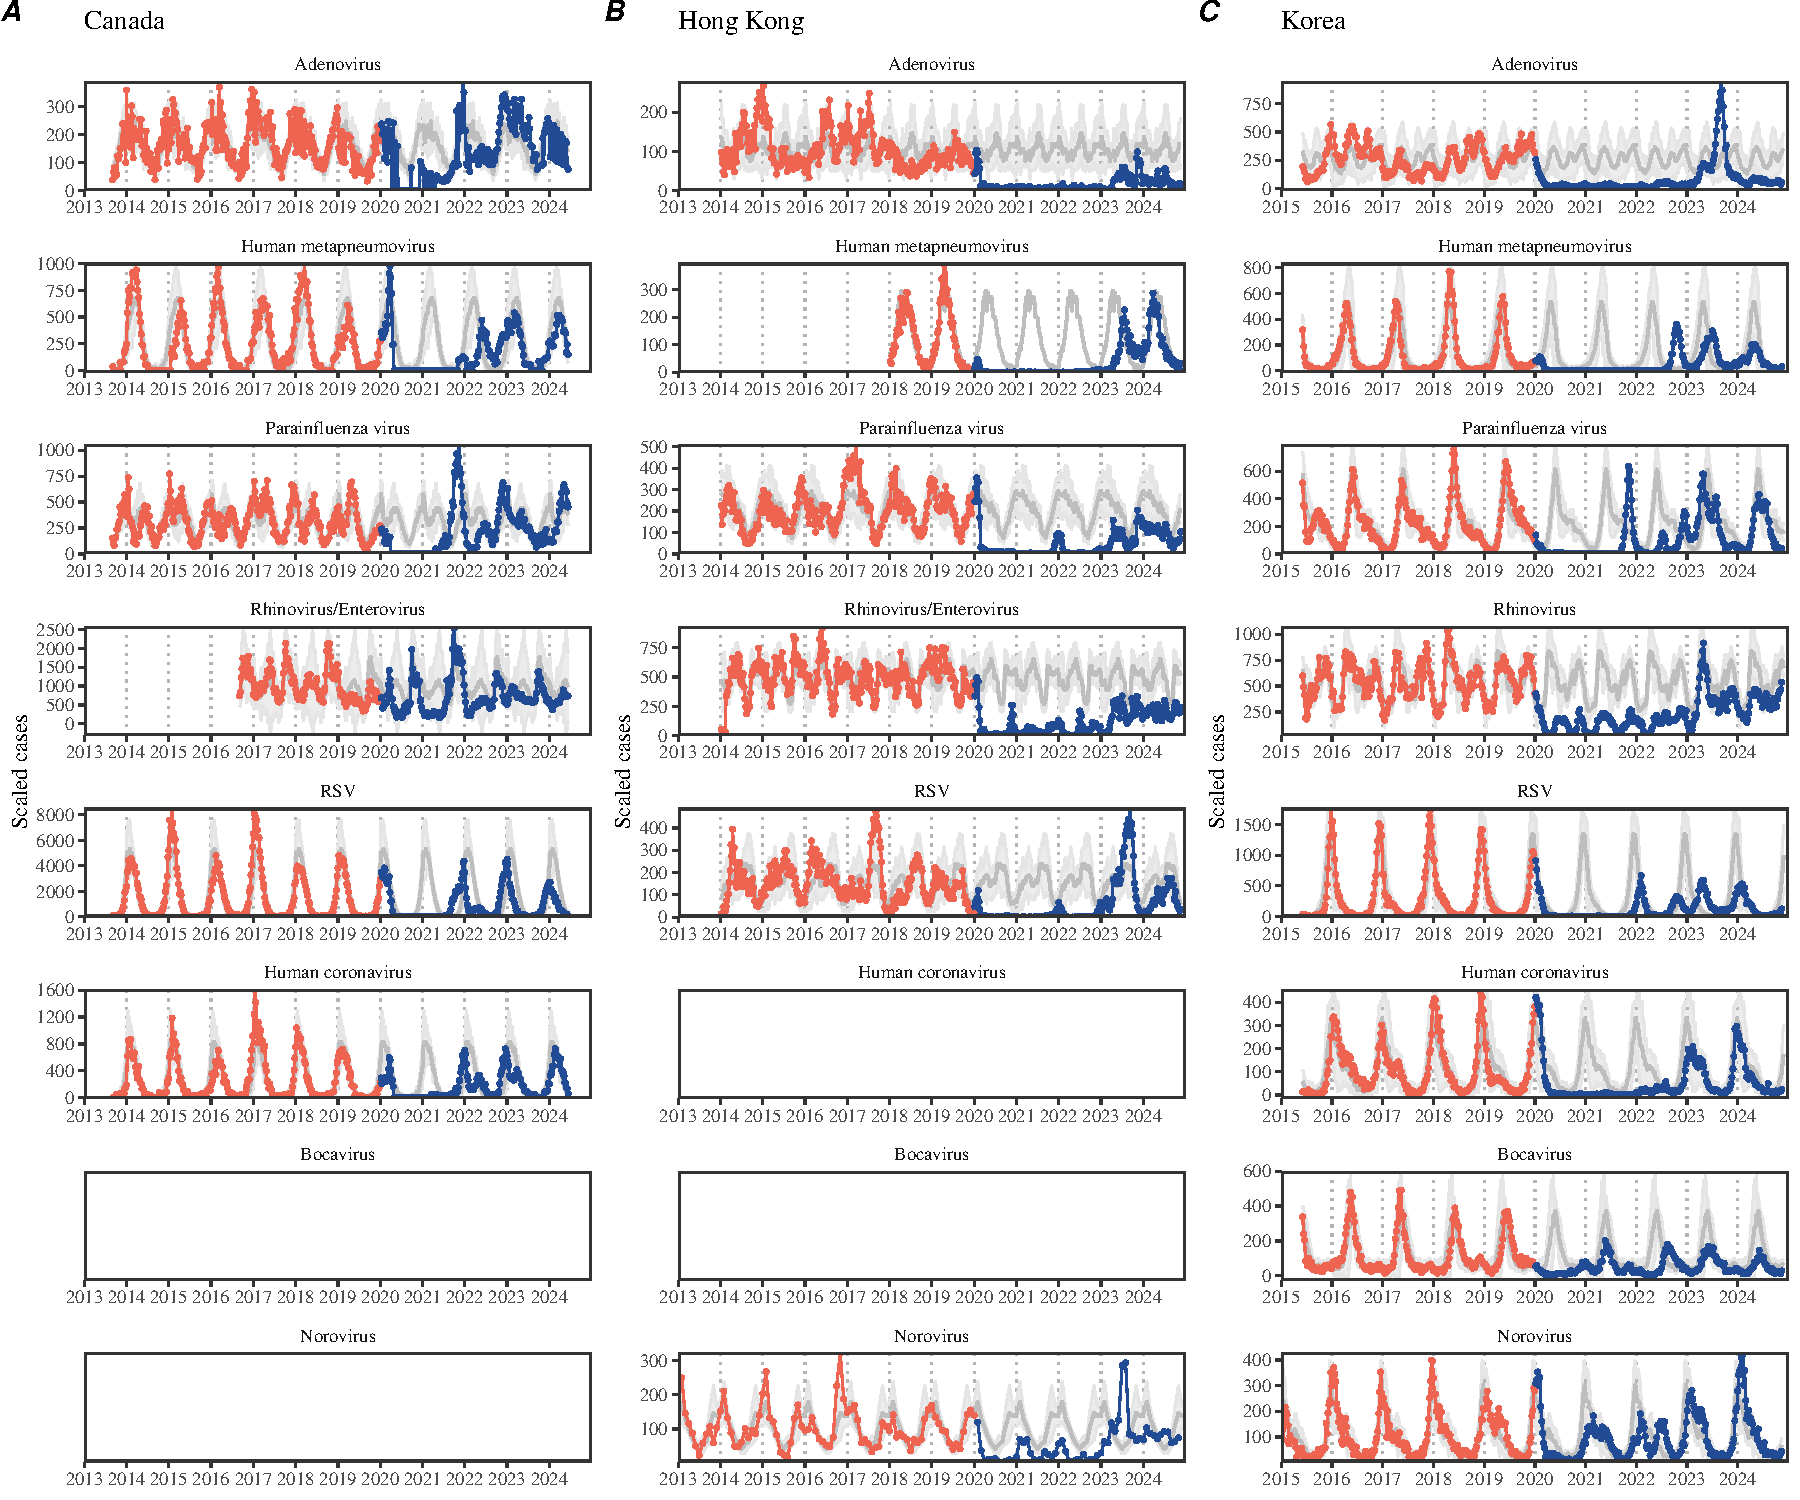
\includegraphics[width=\textwidth]{../figure1/figure1.pdf}
\caption{
\textbf{Observed heterogeneity in responses to pandemic perturbations across respiratory pathogens and norovirus in (A) Canada, (B) Hong Kong, (C) Korea, and (D) US.}
Red points and lines represent data before 2020.
Blue points and lines represent data since 2020.
Gray lines and shaded regions represent the mean seasonal patterns and corresponding 95\% confidence intervals around the mean.
Mean seasonal patterns were calculated by aggregating cases before 2020 into 52 weekly bins and taking the average in each week.
Cases were scaled to account for changes in testing patterns (Materials and Methods).
}
\end{figure} 

Even though more than five years have passed since the emergence of SARS-CoV-2, we still observe persistent changes in pathogen dynamics following the pandemic perturbations.
For example, compared to pre-pandemic, seasonal patterns, human metapneumovirus in Korea seems to circulate at lower levels, whereas RSV in Korea seems to exhibit different seasonality (Figure 1).
These observations suggest a fundamental change in pathogen dynamics following the pandemic perturbations, which might be driven by a long-term shift in either human behavior or population-level immunity \citep{kissler2020projecting,baker2022long}.
For example, the emergence of SARS-CoV-2 could have caused a long-term shift in population-level immunity through its interactions with other pathogens \citep{swets2022sars}, especially with seasonal coronaviruses \citep{kissler2020projecting,lin2022pre,murray2023impact}.
The possibility of a long-lasting impact of the pandemic perturbations poses an important question for future infectious disease dynamics: can we predict whether and when other pathogens will eventually return to their pre-pandemic dynamics?

So far, most analyses of respiratory pathogens after pandemic perturbations have focused on characterizing the timing of rebound \citep{baker2020impact,eden2022off,perofsky2024impacts}.
Instead, we seek to characterize how fast (and whether) a pathogen returns to its pre-pandemic dynamics.
These two concepts have a subtle but important difference. 
For example, it took more than 3 years for human metapneumovirus to rebound in Hong Kong, but the observed epidemic patterns in 2024 appear similar to pre-pandemic seasonal means, suggesting a possible return to pre-pandemic dynamics, though confirmation may require multiple seasons (Figure 1).
Measuring this rate of return is useful because it allows us to quantify the ecological resilience of a host-pathogen system, which can inform responses to future interventions \citep{pimm1979structure, neubert1997alternatives,gunderson2000ecological,dakos2022ecological}.

In this study, we lay out theoretical and statistical approaches to characterizing the resilience of a host-pathogen system based on how fast the system recovers from perturbation.
We begin by laying out a few representative scenarios that capture the potential impact of pandemic perturbations on endemic pathogen dynamics and illustrate how resilience can be measured by comparing the pre- and post-pandemic dynamics of susceptible and infected hosts.
In practice, information on susceptible hosts is often unavailable, making this theoretical approach infeasible.
Instead, we utilize a mathematical technique to reconstruct empirical attractors from the data \citep{takens2006detecting}, which allows us to measure the rate at which the host-pathogen system approaches this empirical attractor after a perturbation;
we define this rate to be the empirical resilience of the host-pathogen system.
We use this method to analyze pathogen surveillance data for respiratory and non-respiratory pathogens from Canada, Hong Kong, Korea, and the US.
Finally, we show that susceptible host dynamics explain variation in pathogen resilience and further demonstrate that more resilient pathogens will be less sensitive to perturbations caused by demographic stochasticity, thereby providing a direct link between pathogen resilience and persistence. 
 
\section*{Conceptual introduction to pathogen resilience}

In classical ecological literature, the resilience of an ecological system is measured by the rate at which the system returns to its reference state following a perturbation \citep{pimm1979structure, neubert1997alternatives,gunderson2000ecological,dakos2022ecological}.
This rate corresponds to the largest real part of the eigenvalues of the linearized system near equilibrium---here, we refer to this value as the \emph{intrinsic} resilience of the system, which represents the expected rate of return from perturbed states.
In practice, we rarely know the true model describing population-level dynamics of common respiratory pathogens, limiting our ability to infer the intrinsic resilience of a system.
Instead, we can measure the \emph{empirical} resilience of a host-pathogen system by looking at how fast the system returns to the pre-perturbation, endemic dynamics after the perturbation has ended.
The COVID-19 pandemic provides a particularly useful example of a major perturbation, providing unqiue opportunities to measure the resilience of a host-pathogen system.

\textbf{Resilience of a single-strain system.} As an example, we begin with a simple Susceptible-Infected-Recovered-Susceptible (SIRS) model with seasonally forced transmission and demography (i.e., birth and death).
The SIRS model is the simplest model that allows for the waning of immunity and is commonly used for modeling the dynamics of respiratory pathogens \citep{dushoff2004dynamical}.
First, consider a pandemic perturbation that reduces transmission by 50\% for 6 months starting in 2020, which causes epidemic patterns to deviate from their original stable annual cycle for a short period of time and eventually come back (Figure 2A).
To measure the resilience of this system empirically, we first need to be able to measure the distance from its pre-pandemic attractor, which is defined as a set of points in state space or phase plane that the system is pulled towards \citep{hastings1993chaos}.
There are many ways we can measure the distance from the attractor, but for illustrative purposes, we choose one of the most parsimonious approaches: that is, we look at how the susceptible (S) and infected (I) populations change over time and measure the Euclidean distance on the SI phase plane, using the counterfactual unperturbed phase plane as a reference (Figure 2B; Materials and Methods).
In this simple case, the locally estimated scatterplot smoothing (LOESS) fit indicates that the distance from the attractor decreases exponentially (linearly on a log scale) on average (Figure 2C).
Furthermore, the overall rate of return approximates the intrinsic resilience of the seasonally unforced system (Figure 2C).

\begin{figure}[!th]
\begin{center}
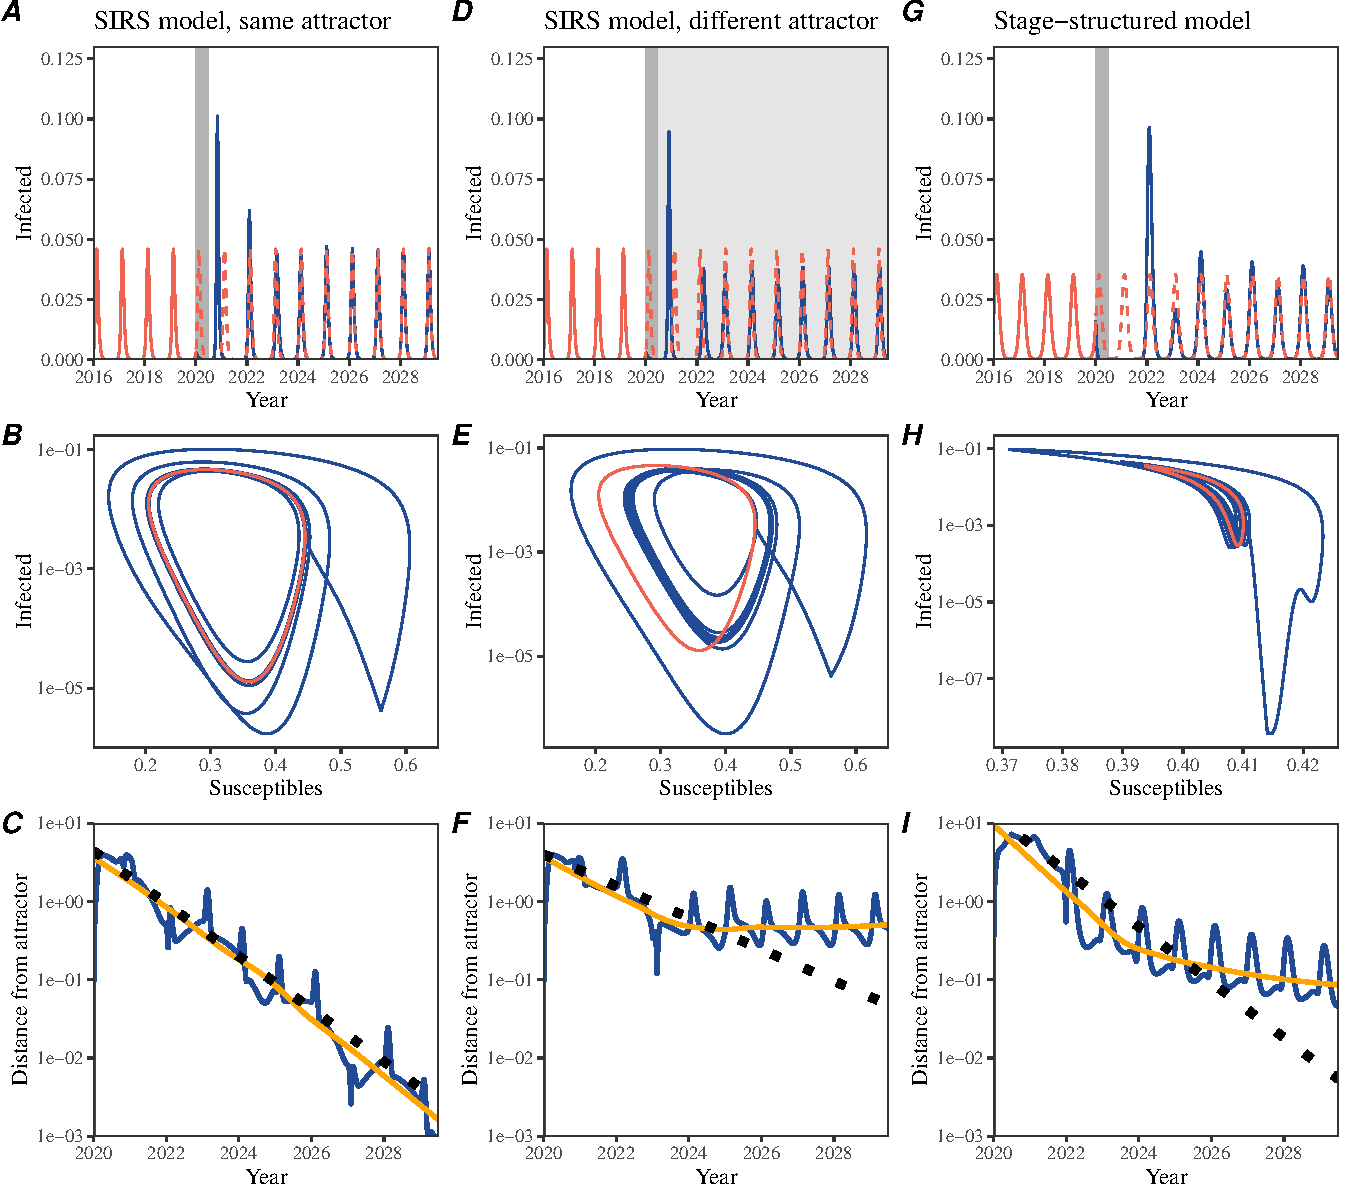
\includegraphics[width=0.9\textwidth]{../figure2/figure2_simple.pdf}
\caption{
\textbf{A simple method to measure pathogen resilience following pandemic perturbations across different scenarios.}
(A, D, G) Simulated epidemic trajectories across various models. 
Red and blue solid lines represent epidemic dynamics before and after pandemic perturbations are introduced, respectively.
Red dashed lines represent counterfactual epidemic dynamics in the absence of perturbations.
Gray regions indicate the duration of perturbations with the dark gray region representing a 50\% transmission reduction and the light gray region representing a 10\% transmission reduction.
(B, E, H) Phase plane representation of the time series in panels A, D, and G alongside the corresponding susceptible host dynamics.
Red and blue solid lines represent epidemic trajectories on an SI phase plane before and after perturbations are introduced, respectively.
(C, F, I) Changes in distance from the attractor over time on a log scale.
Blue lines represent the distance from the attractor.
Orange lines represent the locally estimated scatterplot smoothing (LOESS) fits to the logged distance from the attractor.
Dotted lines show the intrinsic resilience of the seasonally unforced system.
}
\end{center}
\end{figure}

Alternatively, pandemic perturbations can have a lasting impact on the forces driving pathogen dynamics through a long-term reduction in transmission or permanent change in immunity.
As an example, we consider a scenario in which a 10\% reduction in transmission persists even after the major pandemic perturbations are lifted (Figure 2D--F).
In such cases, we cannot know whether the pathogen will return to its original cycle or a different cycle until many years have passed, and we cannot measure the distance to the new unknown attractor that the system might eventually approach.
Nonetheless, we can still measure the distance from the pre-pandemic attractor and ask how the distance changes over time (Figure 2E).
The LOESS fit suggests that the distance from the pre-pandemic attractor will initially decrease exponentially on average (equivalently, linearly on a log scale) and eventually plateau (Figure 2F).
Here, a permanent 10\% reduction in transmission rate slows the system, which causes the distance from the pre-pandemic attractor initially to decrease at a slower rate (Figure 2F) than it would have otherwise (Figure 2C) before plateauing at a fixed distance between the two attractors.
This example shows that resilience is not necessarily an intrinsic property of a specific pathogen.
Instead, pathogen resilience is a property of a specific attractor that a host-pathogen system approaches, which depends on both pathogen and host characteristics.

Finally, transient phenomena can further complicate the picture (Figure 2G--I).
For example, a stage-structured model, which accounts for reduction in secondary susceptibility, initially exhibits a stable annual cycle, but perturbations from a 10\% reduction in transmission for 6 months cause the epidemic to shift to biennial cycles (Figure 2G).
The system eventually approaches the original pre-pandemic attractor (Figure 2H), suggesting that this biennial cycle is a transient phenomenon.
The LOESS fit indicates that the distance from the attractor initially decreases exponentially at a rate that is consistent with the intrinsic resilience of the seasonally unforced stage-structured system, but the approach to the attractor slows down with the damped oscillations (Figure 2I).
This behavior is also referred to as a ghost attractor, which causes long transient dynamics and slow transitions \citep{hastings2018transient}.
Strong seasonal forcing in transmission can also lead to transient phenomena for a simple SIRS model, causing a slow return to pre-perturbation dynamics (Supplementary Figure S1).

\textbf{Resilience of a two-strain system.} This empirical approach allows us to measure the resilience of a two-strain host-pathogen system as well even when we have incomplete observation of the infection dynamics.
Simulations from a simple two-strain competition system illustrate that separate analyses of individual strain dynamics (e.g., RSV A vs B) and a joint analysis of total infections (e.g., total RSV infections) yield identical resilience estimates (Supplementary Figure S2, 3).
This is expected because eigenvalues determine the dynamics of the entire system around the equilibrium, meaning that both strains should exhibit identical rates of return following a perturbation.
However, these conclusions likely depend on the strength of strain interaction as well as the underlying details of the model.
For example, ecological interferences between two unrelated pathogens \citep{rohani2003ecological} will likely generate weaker coupling than cross immunity between related pathogens;
in the former case, we do not necessarily expect two unrelated pathogens to have same resilience despite their ecological interferences.
For simplicity, we focus on a simple, two-strain model with cross immunity in this paper.
Analogous to a single-strain system, strong seasonal forcing in transmission can cause the two-strain system to slow down through transient phenomena (Supplementary Figure S4).

These observations yield three insights.
First, we can directly estimate the empirical resilience of a host-pathogen system by measuring the rate at which the system approaches an attractor, provided that we have a way to quantify the distance from the attractor---as we discuss later, the attractor of a system can be reconstructed from data from mathematical theory without making assumptions about the underlying model.
The empirical approach to estimating pathogen resilience is particularly convenient because it does not require us to know the true underlying model;
estimating the intrinsic resilience from fitting misspecified models can lead to biased estimates (Supplementary Figure S5).
Second, resilience estimates allow us to make phenomenological predictions about the dynamics of a host-pathogen system following a perturbation.
Assuming that an attractor has not changed and the distance from the attractor will decrease exponentially over time, we can estimate when the system should reach an attractor.
Finally, a change in the (exponential) rate of approach provide information about whether the system has reached an alternative attractor, or a ghost attractor, that is different from the original, pre-pandemic attractor.
These alternative attractors may reflect permanent changes in transmission patterns as well as changes in immune landscapes.
There will be periods of time when it is difficult to tell whether pathogen dynamics are still diverging from the original attractor due to a long-term perturbation, or have entered the basin of attraction of a new attractor. 
Now that several years have passed since major interventions have been lifted, many respiratory pathogens may have had sufficient time to begin returning to their post-intervention attractors---empirical comparisons between current cases and pre-pandemic cases are consistent with this hypothesis (Figure 1).
With recent data, we can start to evaluate whether we see early signs of convergence to the former attractor or a new one.

\section*{Inferring pathogen resilience from real data}

Based on these observations, we now lay out our approach to estimating pathogen resilience from real data (Figure 3).
We first tested this approach against simulations and applied it to real data.
Specifically, we analyzed case time series of respiratory pathogens from four countries: Canada, Hong Kong, Korea, and the US.

So far, we have focused on simple examples that assume a constant transmission reduction during the pandemic.
However, in practice, the impact of pandemic perturbations on pathogen transmission was likely more complex (Figure 3A), reflecting introduction and relaxation of various intervention strategies.
In some cases, strong perturbations likely caused local fadeouts, requiring immigration/importation from another location for epidemic rebound.
Such complexities could lead to longer delays between the introduction of pandemic perturbations and pathogen rebound as well as temporal variation in outbreak sizes (Figure 3B);
in this example, continued transmission reduction from interventions limits the size of the first outbreak in 2021 following the rebound, allowing for a larger outbreak in 2022 when interventions are further relaxed.

Previously, we relied on the dynamics of susceptible and infected hosts to compute the distance from the attractor (Figure 2), but information on susceptible hosts is rarely available in practice.
In addition, uncertainties in case counts due to observation error, strain evolution, and multiannual cycles in the observed epidemic dynamics (e.g., adenovirus circulation patterns in Hong Kong and Korea) add challenges to defining pre-pandemic attractors, which limits our ability to measure the distance from the attractor.
To address these challenges, we can reconstruct an empirical attractor by utilizing Takens' theorem \citep{takens2006detecting}, which states that an attractor of a nonlinear multidimensional system can be mapped onto a delayed embedding (Materials and Methods).
For example, we can use delayed logged values of pre-pandemic cases $C(t)$ (Figure 3C) to reconstruct the attractor:
\begin{equation}
\langle\log(C(t)+1), \log(C(t-\tau)+1), \dots, \log(C(t-(M-1)\tau)+1)\rangle,
\end{equation}
where the delay $\tau$ and embedding dimension $M$ are determined based on autocorrelations and false nearest neighbors, respectively \citep{kennel1992determining,tan2023selecting}.
This allows us to define the pre-pandemic attractor as a points on an $M$ dimensional space.
We can then apply the same delay and embedding dimensions to the entire time series to determine the position in multi-dimensional state space (Figure 3D), which allows us to measure the nearest neighbor distance between the current state of the system and the empirical pre-pandemic attractor (Figure 3E).
Specifically, the nearest neighbor distance is calculated by computing the distance between the current poisition on the $M$ dimensional space and all points in the empirical attractor set and taking the minimum value.
In theory, we can now quantify how fast this distance decreases by fitting a linear regression on a log scale, where the slope of the linear regression empirically measures pathogen resilience with a steeper slope corresponding to a higher resilience estimate (Figure 3E).
However, resulting estimates of pathogen resilience can be sensitive to choices about embedding delays and dimensions.
For example, using longer delays and higher dimensions tends to smooth out temporal variations in the distance from the attractor (Supplementary Figure S6).

\begin{figure}[!ht]
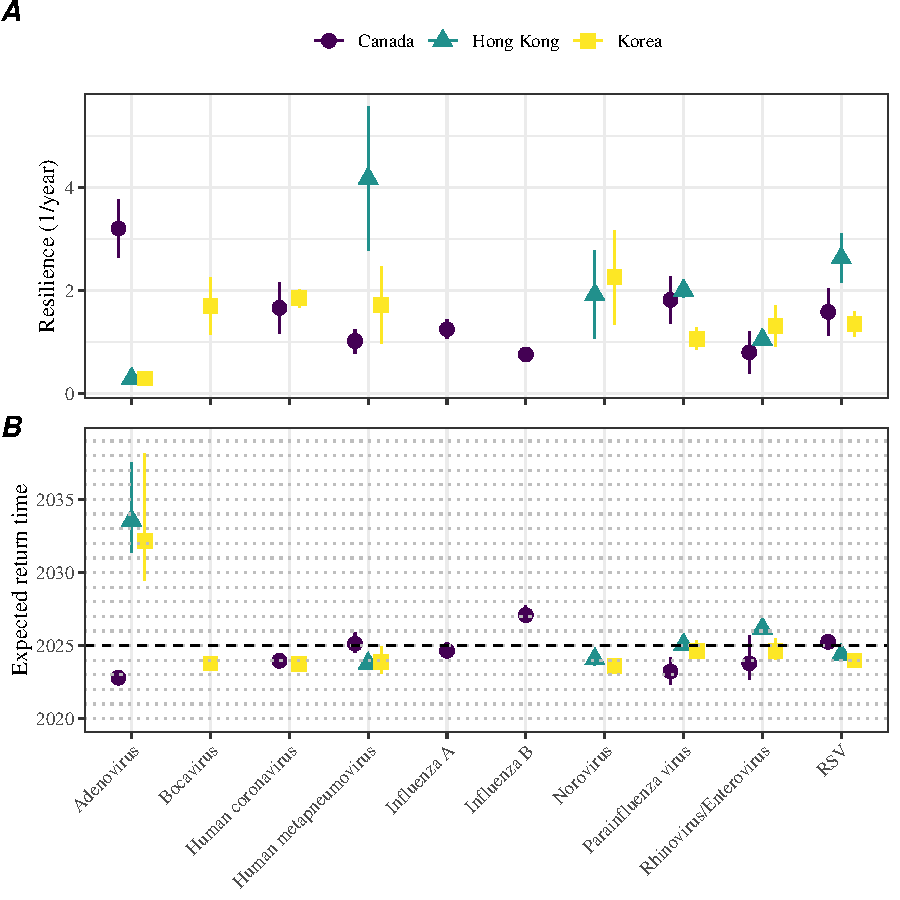
\includegraphics[width=\textwidth]{../figure3/figure3.pdf}
\caption{
\textbf{A schematic diagram explaining the inference of pathogen resilience from synthetic data.}
(A) A realistic example of simulated pandemic perturbations, represented by a relative reduction in transmission.
(B) The impact of the synthetic pandemic perturbation on epidemic dynamics simulated using a SIRS model with demographic stochasticity.
(C) Generating delayed copies of the logged time series allows us to obtain an embedding.
(D) Two dimensional representation of an embedding.
(E) Delayed embedding allows us to calculate the nearest neighbor distance from the empirical attractor, which is determined based on the pre-pandemic time series.
Blue lines and dashed regions represent the linear regression fit and the associated 95\% confidence interval.
This distance time series can be used to infer pathogen resilience after choosing an appropriate window for linear regression.
For illustration purposes, an arbitrary fitting window was chosen.
}
\end{figure}

Complex changes in the distance from the attractor suggest that estimating pathogen resilience from linear regression will be particularly sensitive to our choice of fitting windows for the regression (Figure 3E).
Therefore, before we tried estimating resilience from real data, we explored an automated window selection criterion for linear regression and tested it against randomized, stochastic simulations across a range of realistic pandemic perturbation shapes.
In doing so, we also explored optimal choices for embedding dimensions and evaluated our choices of fitting window parameters and embedding dimensions by quantifying correlation coefficients between the estimated resilience and the intrinsic resilience of a seasonally unforced system (Materials and Methods).
Overall, we found large variation in estimation performances with correlation coefficient ranging from 0.21 to 0.61 (Supplementary Figure S7).
In almost all cases, the automated window selection approach outperformed a naive approach, which performs regression between the peak distance and current distance (Supplementary Figure S7).

Based on the best performing window selection criteria and embedding dimension, we applied this approach to pathogen surveillance data presented in Figure 1 (Materials and Methods).
For each time series, we applied Takens' theorem independently to reconstruct the empirical attractor and obtained the corresponding time series of distances from attractors (Supplementary Figure S8).
Then, we used the automated window selection criterion to fit a linear regression and estimated the empirical resilience for each pathogen in each country (Supplementary Figure S8);
the window selection criterion gave poor regression window for three cases (norovirus in Hong Kong and Korea and rhinovirus/enterovirus in the US), leading to unrealistically low resilience estimates, and so we used ad-hoc regression windows instead (Supplementary Figure S9; Materials and Methods).

For all pathogens we considered, resilience estimates fell between $0.4/\mathrm{year}$ and $1.8/\mathrm{year}$ (Figure 4A).
We estimated the mean resilience of common respiratory pathogens to be $0.99/\mathrm{year}$ (95\% CI: $0.81/\mathrm{year}$--$1.18/\mathrm{year}$).
For reference, this is $\approx 7.5$ times higher than the intrinsic resilience of pre-vaccination measles in England and Wales ($\approx 0.13/\mathrm{year}$).
Finally, resilience estimates for norovirus, a gastrointestinal pathogen, were comparable to those of common respiratory pathogens: $1.44/\mathrm{year}$ (95\% CI: $1.01/\mathrm{year}$--$1.87/\mathrm{year}$) for Hong Kong and $1.07/\mathrm{year}$ (95\% CI: $0.86/\mathrm{year}$--$1.29/\mathrm{year}$) for Korea.
Based on a simple ANOVA test, we did not find significant differences in resilience estimates across countries ($p=0.25$) or pathogens ($p=0.67$).

\begin{figure}[!th]
\begin{center}
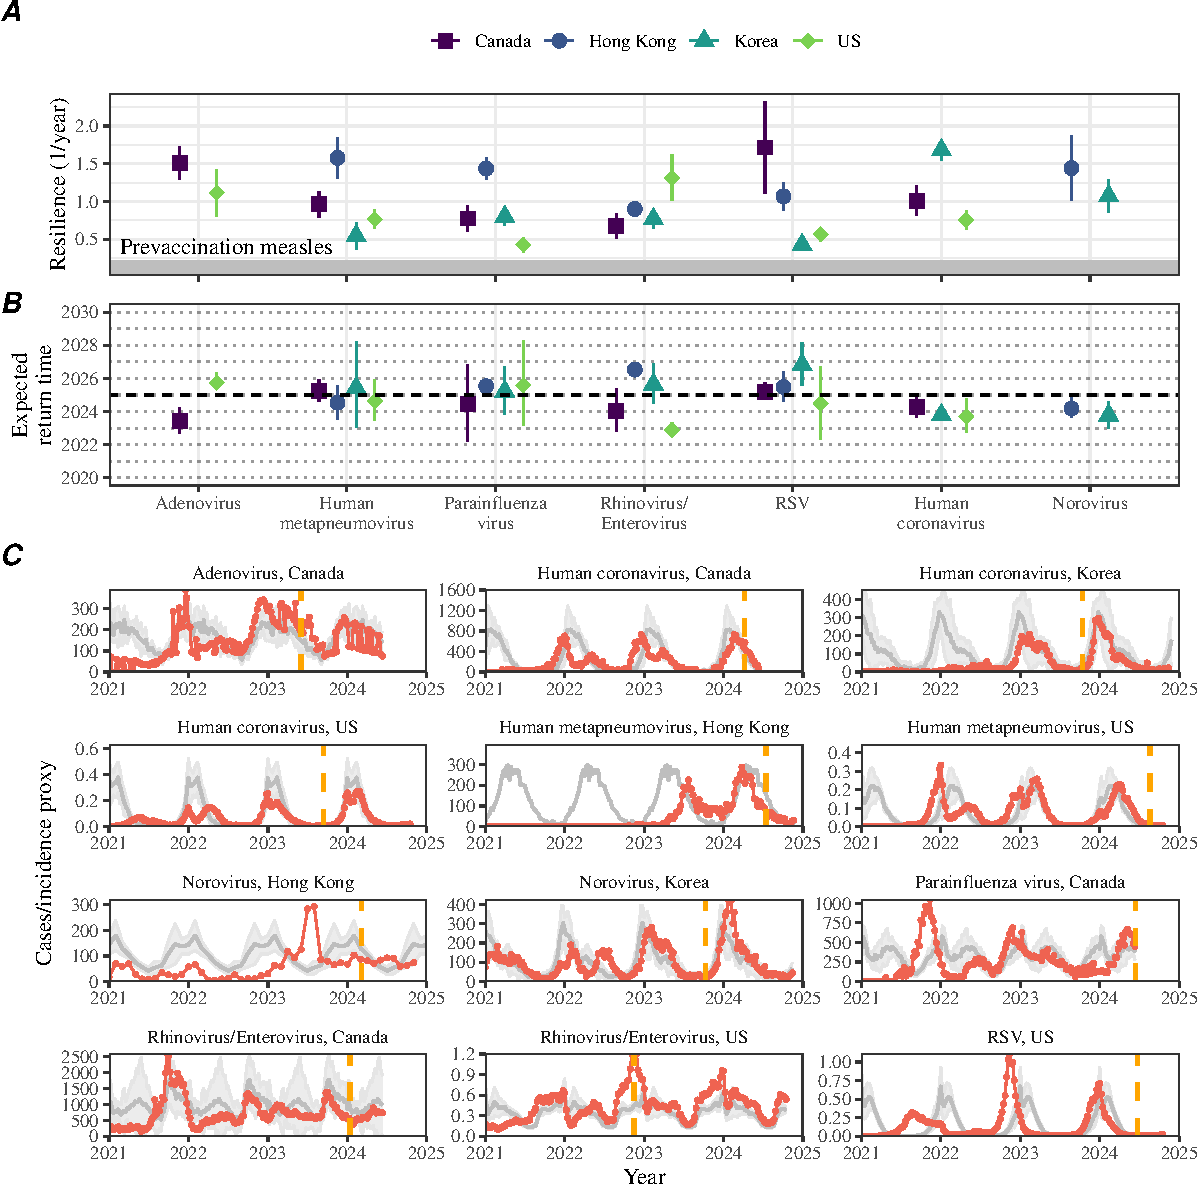
\includegraphics[width=0.8\textwidth]{../figure4/figure4.pdf}
\caption{
\textbf{Summary of resilience estimates and predictions for return time.}
(A) Estimated pathogen resilience.
The gray horizontal line represents the intrinsic resilience of pre-vaccination measles dynamics.
(B) Predicted timing of when each pathogen will return to their pre-pandemic cycles.
The dashed line in panel B indicates the end of 2024.
Error bars represent 95\% confidence intervals.
(C) Observed dynamics for pathogen that are predicted to have returned before the end of 2024.
Red points and lines represent data before 2020.
Gray lines and shaded regions represent the mean seasonal patterns and corresponding 95\% confidence intervals around the mean, previously shown in Figure 1.
Orange vertical lines represent the predicted timing of return.
}
\end{center}
\end{figure}

Using resilience estimates, we predicted when each pathogen would hypothetically return to their pre-pandemic dynamics, assuming no long-term change in the attractor.
Specifically, we extended our linear regression fits to distance-from-attractor time series and ask when the predicted regression line will cross a threshold value;
since we relied on nearest neighbor distances, pre-pandemic distances are always greater than zero (Figure 3E), meaning that we can use the mean of pre-pandemic distances as our threshold.

We predicted that a return to pre-pandemic cycles has occurred or would be imminent for most pathogens (Figure 4B).
In particular, we predicted that 12 out of 23 pathogen-country pairs should have already returned before the end of 2024.
For almost all pathogens that were predicted to have returned already, the observed epidemic dynamics showed clear convergence towards their pre-pandemic seasonal averages, confirming our predictions (Figure 4C).
However, there were a few exceptions, including norovirus in Hong Kong and rhinovirus/enterovirus in the US, where the observed epidemic dynamics in 2024 exhibit clear deviation from their pre-pandemic seasonal averages (Figure 4C; Figure S9).
These observations suggest a possibility that some common respiratory pathogens may have converged to different attractors or are still exhibiting non-equilibrium dynamics.
In contrast, pathogens that were predicted to have not returned yet also showed clear differences from their pre-pandemic seasonal averages; as many of these pathogens are predicted to return in 2025--2026, we may be able to test these predictions in near future (Supplementary Figure S10).
Our reconstructions of distance time series and estimates of pathogen resilience and expected return time were generally robust to choices of embedding dimensions (Supplementary Figure S11--12).

\section*{Susceptible host dynamics explain variation in pathogen resilience}

So far, we have focused on quantifying pathogen resilience from the observed patterns of pathogen re-emergence following pandemic perturbations.
But what factors determine how resilient a host-pathogen system is?
To address this question, we used the SIRS model to explore how changes in susceptible host dynamics affect pathogen resilience.
To do so, we varied the basic reproduction number $\mathcal R_0$, which represents the average number of secondary infections caused by a newly infected individual in a fully susceptible population, and the duration of immunity and computed intrinsic resilience for each parameter.

\begin{figure}[!th]
\begin{center}
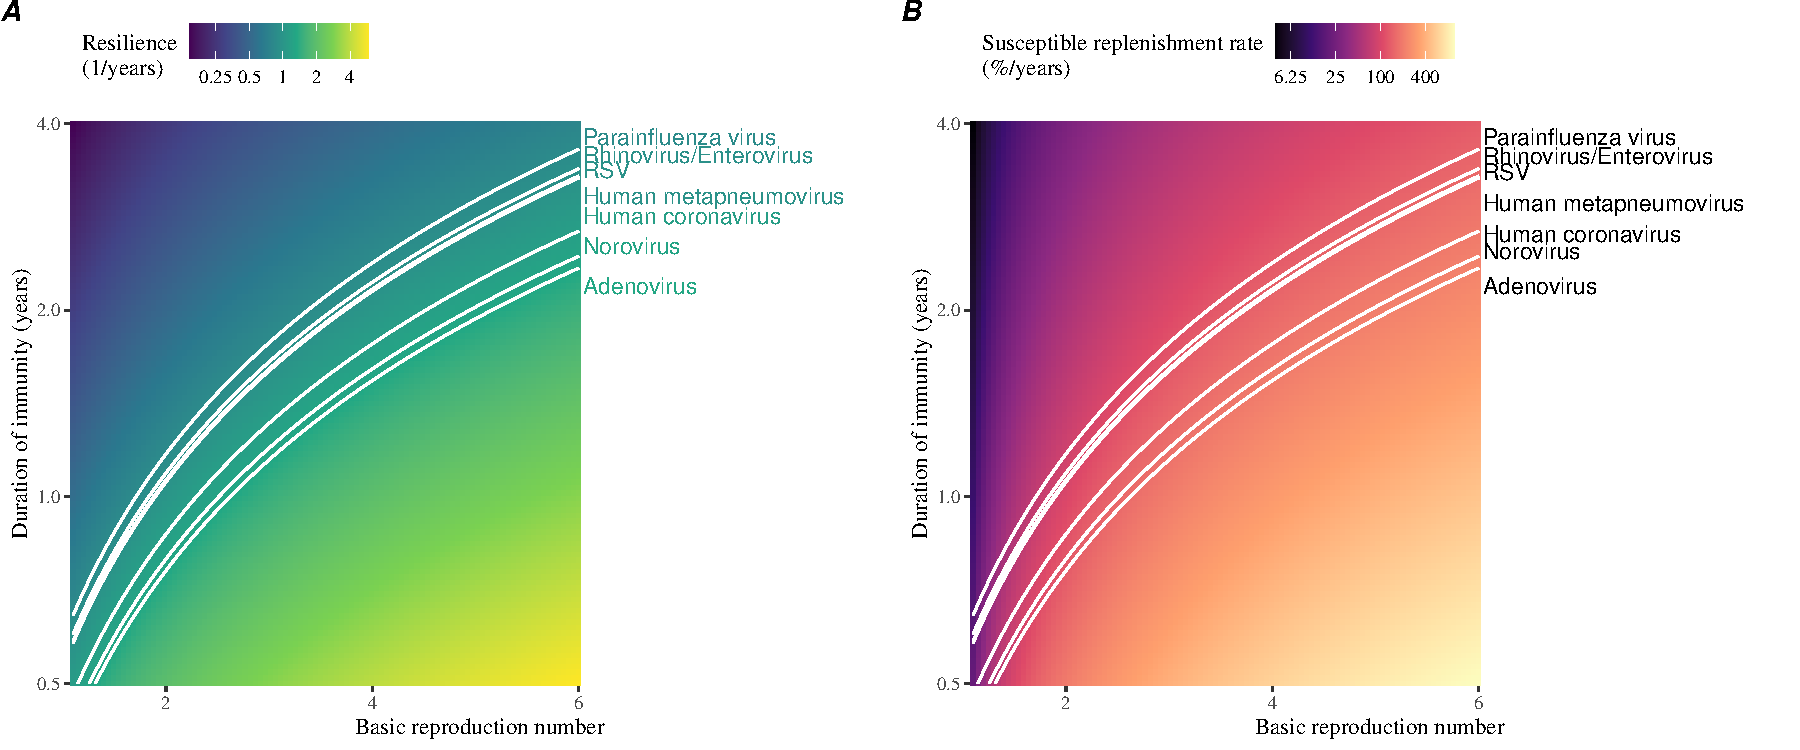
\includegraphics[width=\textwidth]{../figure5/figure5.pdf}
\caption{
\textbf{Linking pathogen resilience to epidemiological parameters and susceptible host dynamics.}
(A) Intrinsic resilience as a function of the basic reproduction number $\mathcal R_0$ and the duration of immunity.
(B) Per-capita susceptible replenishment rate as a function of the basic reproduction number $\mathcal R_0$ and the duration of immunity.
The standard SIRS model without seasonal forcing is used to compute intrinsic resilience and the per-capita susceptible replenishment rate.
Lines correspond to a set of parameters that are consistent with mean resilience estimates for each pathogen, averaged across different countries.
}
\end{center}
\end{figure}

We found that an increase in $\mathcal R_0$ and a decrease in the duration of immunity correspond to an increase in pathogen resilience (Figure 5A).
Similarly, an increase in $\mathcal R_0$ and a decrease in the duration of immunity corresponds to a faster per-capita rate of susceptible replenishment, which is defined as the ratio between absolute rate at which new susceptibles enter the population and the equilibrium number of susceptible individuals in the population, $S^\ast$ (Figure 5B).
We note that a higher $\mathcal R_0$ drives a faster per-capita susceptible replenishment rate by decreasing the susceptible proportion at equilibrium, $S^\ast$.
For a simple SIR model that assumes a life-long immunity, we can show analytically that pathogen resilience is proportional to the per-capita rate of susceptible replenishment (Materials and Methods).
Overall, these observations suggest that a faster per-capita susceptible replenishment rate causes the system to be more resilient.

By taking the average values of empirical resilience values for each pathogen, we were able to map each pathogen onto a set of parameters of the SIRS model that are consistent with corresponding resilience estimates (Figure 5A).
Across all pathogens we considered, we estimated that the average duration of immunity is likely to be short ($<4$ years) across a plausible range of $\mathcal R_0$ ($<6$).
We were also able to obtain a plausible range of susceptible replenishment rates for each pathogen (Figure 5B), but there was a large uncertainty in the estimates for susceptible replenishment rates due to a lack of one-to-one correspondence between susceptible replenishment rates and pathogen resilience.

\section*{Pathogen resilience determines sensitivity to stochastic perturbations}

Even in the absence of major pandemic perturbations, host-pathogen systems are expected to experience continued perturbations of varying degrees from changes in epidemiological conditions, such as human behavior, climate, and viral evolution.
These perturbations can also arise from demographic stochasticity, which is inherent to any ecological systems.
Here, we used a seasonally unforced SIRS model with birth/death to explore how resilience of a host-pathogen system determines the sensitivity to perturbations caused by demographic stochasticity (Materials and Methods).

\begin{figure}[!th]
\begin{center}
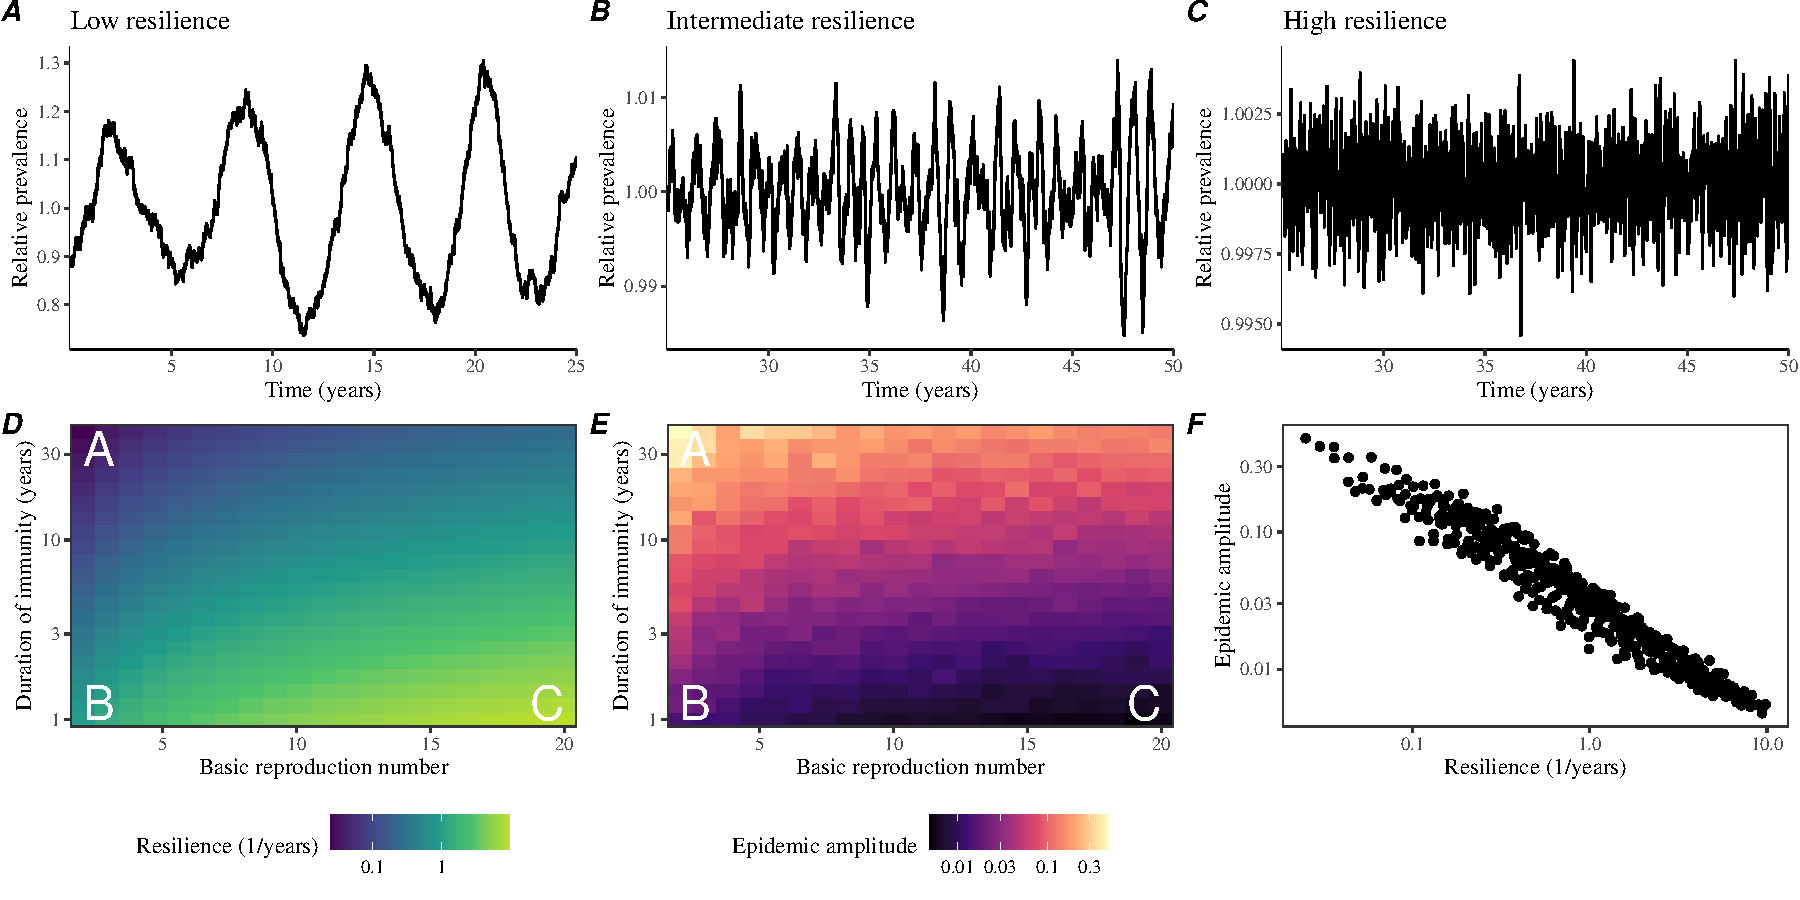
\includegraphics[width=\textwidth]{../figure6/figure_persistence_noise.pdf}
\caption{
\textbf{Linking resilience of a host-pathogen system to its sensitivity to stochastic perturbations.}
(A--C) Epidemic trajectories of a stochastic SIRS model across three different resilience values: low, intermediate, and high.
The relative prevalence was calculated by dividing infection prevalence by its mean value.
(D) Intrinsic resilience of a system as a function of the basic reproduction number $\mathcal R_0$ and the duration of immunity.
(E) Epidemic amplitude as a function of the basic reproduction number $\mathcal R_0$ and the duration of immunity.
The epidemic amplitude corresponds to $(\max I - \min I)/(2 \bar{I})$, where $\bar{I}$ represents the mean prevalence.
Labels A--C in panels D and E correspond to scenarios shown in panels A--C.
(F) The relationship between pathogen resilience and epidemic amplitude.
}
\end{center}
\end{figure}

We found that resilience of a host-pathogen system determines the amount of deviation from the deterministic trajectory caused by demographic stochasticity, with less resilient systems experiencing larger deviations (Figure 6).
Notably, less resilient systems also exhibited slower epidemic cycles (Figure 6A--C). 
The periodicity of this epidemic cycle matched those predicted by the intrinsic periodicity of the system (Supplementary Figure S13) where the intrinsic resilience of the system is inversely proportional to its intrinsic periodicity (Supplementary Figure S14).
However, we note that the interplay between seasonal transmission and intrinsic periodicity can also lead to complex cycles, as illustrated by a recent analysis of \textit{Mycoplasma pneumoniae} dynamics \citep{nielsen2025complex}.

We also note that the intrinsic resilience is not the sole determinant for how sensitive the system is to stochastic perturbations.
For example, the population size and average duration of infection also affect the amount of deviation from the deterministic trajectory caused by demographic stochasticity, even though these quantities have little to no impact on the intrinsic resilience (Supplementary Figure S15).
These conclusions were robust for the seasonally forced SIRS model (Supplementary Figure S16).

\section*{Discussion}

COVID-19 pandemic interventions caused major disruptions to circulation patterns of both respiratory and non-respiratory pathogens, adding challenges to predicting their future dynamics \citep{baker2020impact,gomez2021uncertain,koltai2022determinants,park2024predicting}.
However, these perturbations offer large-scale natural experiments for understanding how different pathogens respond to perturbations.
In this study, we showed that pathogen re-emergence patterns following pandemic perturbations can be characterized through the lens of ecological resilience and presented a new method for estimating pathogen resilience from time series data.
We showed that variation in pathogen resilience can be explained by the differences in susceptible host dynamics, where faster replenishment of the susceptible pool corresponds to a more resilient host-pathogen system.
Finally, we showed that pathogen resilience also determines the sensitivity to stochastic perturbations.

We analyzed case time series of common respiratory infections and norovirus infections from Canada, Hong Kong, Korea, and the US to estimate their resilience.
Overall, we estimated the resilience of these pathogens to range from $0.4/\mathrm{year}$ to $1.8/\mathrm{year}$, which is 3--14 times more resilient than prevaccination measles.
Consistent with other epidemiological evidence \citep{bosis2008role,o2009symptomatic,pitzer2015environmental,edridge2020seasonal}, these resilience estimates indicate that common respiratory pathogens and norovirus likely exhibit faster susceptible replenishment and are therefore more persistent, indicating potential challenges in controlling these pathogens.

Based on our resilience estimates, we made phenomenological predictions about when each pathogen will return to their endemic cycles.
For the most part, we accurately predicted which pathogens should have already returned before the end of 2024.
However, there were two main exceptions (i.e., norovirus in Hong Kong and rhinovirus/enterovirus in the US), suggesting that these pathogens may be converging to new endemic cycles or experiencing long-term transient behavior.
These changes may reflect changes in surveillance or actual shift in the dynamics, caused by permanent changes in behavior or population-level immunity.
While it may seem unlikely that permanent changes in behavior would only affect a few pathogens and not others, we cannot rule out this possibility given differences in the observed mean age of infections and therefore the differences in age groups that primarily drive transmission \citep{radin2014epidemiology,lv2024epidemiological}.
Differences in the mode of transmission between respiratory vs gastrointestinal pathogens may also contribute to the differences in responses to pandemic perturbations.

For almost half of the pathogens we considered, we predicted that their return to original epidemic patterns is imminent.
We will need a few more years of data to test whether these pathogens will eventually return to their original dynamics or eventually converge to a different attractor.
We also cannot rule out the possibility that some pathogens may exhibit long-term transient behaviors following pandemic perturbations.
Overall, these observations echo earlier studies that highlighted the long-lasting impact of pandemic perturbations \citep{baker2022long,caini2024probable,chen2024covid,park2024predicting,nielsen2025complex}. 

We showed that susceptible host dynamics shape pathogen resilience, where faster replenishment of the susceptible population causes the pathogen to be more resilient.
For simplicity, we focused on waning immunity and birth as the main drivers of the susceptible host dynamics but other mechanisms can also contribute to the replenishment of the susceptible population.
In particular, pathogen evolution, especially the emergence of antigenically novel strains, can cause effective waning of immunity in the population;
therefore, we hypothesize that the rate of antigenic evolution is likely a key feature of pathogen resilience.
Future studies should explore the relationship between the rate of evolution and resilience for antigenically evolving pathogens.
This result also highlights the importance of detailed measurements of changes in the susceptible population through serological assays for understanding pathogen dynamics \citep{nguyen2022enterovirus}.

Quantifying pathogen resilience also offers novel approaches to validating population-level epidemiological models.
So far, most model validation in infectious disease ecology is based on the ability of a model to reproduce the observed epidemic dynamics and to predict future dynamics \citep{grenfell2002dynamics,bhattacharyya2015cross,pitzer2015environmental,dean2018human,pons2018serotype}.
However, many models can perform similarly under these criteria.
For example, two major RSV models have been proposed to explain biennial epidemic patterns: (1) a stage- and age-structured model that allows disease severity to vary with number of past infections and age of infection \citep{pitzer2015environmental} and (2) a pathogen-interaction model that accounts for cross immunity between RSV and human metapneumovirus \citep{bhattacharyya2015cross}.
Since both models can accurately reproduce the observed epidemic patterns, standard criteria for model validation do not allow us to distinguish between these two models from population-level data alone.
Instead, it would be possible to measure the empirical resilience of each model by simulating various perturbations and comparing the simulations to estimates of empirical resilience from data, using pandemic perturbations as a reference.

There are several limitations to our work.
First, we did not extensively explore other approaches to reconstructing the attractor.
Recent studies showed that more sophisticated approaches, such as using non-uniform embedding, can provide more robust reconstruction for noisy data \citep{tan2023selecting}.
In the context of causal inference, choices about embedding can have major impact on the resulting inference \citep{cobey2016limits}.
Our resilience estimates are likely overly confident given a lack of uncertainties in attractor reconstruction as well as the simplicity of our statistical framework.
Nonetheless, as illustrated in our sensitivity analyses, inferences about pathogen resilience in our SIRS model appear to be robust to decisions about embedding lags and dimensions---this is because tracking the rate at which the system approaches the attractor is likely a much simpler problem than making inferences about causal directionality.
Short pre-pandemic time series also limit our ability to accurately reconstruct the attractor and contribute to the crudeness of our resilience estimates;
although this is less likely a problem for respiratory pathogens that are strongly annual, our attractor reconstruction may be inaccurate for those exhibiting multi-annual cycles, such as adenovirus in Hong Kong and Korea.
Our framework also do not allow us to distinguish whether a system has settled to a new attractor or is experiencing long-term transient behavior.
Uncertainties in pathogen dynamics due to changes in testing patterns further contribute to the crudeness of our resilience estimates.
Despite these limitations, our qualitative prediction that common respiratory pathogens are more resilient than prevaccination measles is also likely to be robust, given how rapidly many respiratory pathogens returned to their original cycles following pandemic perturbations.

While attractor reconstruction methods 

Predicting the impact of anthropogenic changes on infectious disease dynamics is a fundamental aim of infectious disease research in a rapidly changing world.
Our study illustrates that how a host-pathogen system responds to both small and large perturbations is largely predictable through the lens of ecological resilience.
In particular, quantifying the resilience of a host-pathogen system offers a unique insight into questions about endemic pathogens' responses to pandemic perturbations, including whether some pathogens will exhibit long-lasting impact from the pandemic perturbation or not.
More broadly, a detailed understanding of the determinants of pathogen resilience can provide deeper understanding of pathogen persistence.

\section*{Materials and Methods}

\subsection*{Data}

We gathered time series on respiratory infections from Canada, Hong Kong, Korea, and United States (US).
As a reference, we also included time series data on norovirus infections when available.
In contrast to respiratory pathogens, we hypothesized gastrointestinal viruses, such as norovirus, to be differently affected by pandemic perturbations.

Weekly time series of respiratory infection cases in Canada came from a publicly available website by the Respiratory Virus Detection Surveillance System, which collects data from select laboratories across Canada \citep{phac}.
Weekly time series of respiratory infection cases in Hong Kong came from a publicly available website by the Centre for Health Protection, Department of Health \citep{hkdata,hkdata2}.
Weekly time series of acute respiratory infection cases in Korea came from a publicly available website by the Korea Disease Control and Prevention Agency \citep{kordata}.
Finally, weekly time series of respiratory infection cases in the US were obtained from the National Respiratory and Enteric Virus Surveillance System.
Time series on number of tests were also available in Canada, Hong Kong, and the US, but not in Korea.
% \swp{Not sure how to cite NREVSS data because we got it by emailing them...}

\subsection*{Data processing}

For all time series, we rounded every year to 52 weeks by taking the average number of cases and tests between the 52nd and 53rd week.
We also rescaled all time series to account for changes in testing patterns, which were then used for the actual analysis.

For Canada, an increase in testing was observed from 2013 to 2024 (Supplementary Figure S17).
To account for this increase, we calculated a 2 year moving average for the number of tests for each pathogen, which we used as a proxy for testing effort.
Then, we divided the smoothed testing patterns by the smoothed value at the final week such that the testing effort has a maximum of 1.
We then divided weekly cases by the testing effort to obtain a scaled case time series.
A similar approach was used earlier for an analysis of RSV time series in the US to account for changes in testing patterns \citep{pitzer2015environmental}.

For Hong Kong, we applied the same scaling procedure to the time series as we did for Canada.
In this case, we only adjusted for testing efforts up to the end of 2019 because there was a major reduction in testing for common respiratory pathogens between 2020 and 2023 (Supplementary Figure S18).

For Korea, while we did not have information on testing, the reported number of respiratory infections consistently increased from 2013 to the end of 2019, which we interpreted as changes in testing patterns (Supplementary Figure S19).
Since we did not have testing numbers, we used the weekly sum of all acute respiratory viral infection cases as a proxy for testing, which were further smoothed with moving average and scaled to have a maximum of 1.
For Korea, we also only adjusted for testing efforts up to the end of 2019.

In the US, there has been a large increase in testing for some respiratory pathogens, especially RSV, which could not be corrected by simple scaling (Supplementary Figure S20).
Instead, we derived an incidence proxy by multiplying the test positivity with influenza-like illness positivity, which was taken from \url{https://gis.cdc.gov/grasp/fluview/fluportaldashboard.html}.
This method of estimating an incidence proxy has been recently applied in the analysis of seasonal coronaviruses \citep{kissler2020projecting} and \textit{Mycoplasma pneumoniae} infections \citep{park2024predicting}.
Detailed assumptions and justifications are provided in \citep{goldstein2011predicting}.

\subsection*{Data summary}

To make qualitative comparisons between pre- and post-perturbation dynamics of respiratory pathogen circulation patterns, we calculated the mean seasonal patterns using time series of either rescaled cases or incidence proxy estimates before 2020.
We did so by taking the mean value in each week across all years before 2020.
Confidence intervals around the means were calculated using a simple t test.

\subsection*{Estimating pathogen resilience}

In order to measure pathogen resilience from surveillance data, we first reconstructed the empirical pre-pandemic attractor of the system using Takens' embedding theorem \citep{takens2006detecting}.
Specifically, for a given pathogen, we took the pre-pandemic (before 2020) case time series $C(t)$ and reconstructed the attractor using delayed embedding with a uniform delay of $\tau$ and dimension $M$:
\begin{equation}
X_{\tau,m}(t) = \langle\log(C(t)+1), \log(C(t-\tau)+1), \dots, \log(C(t-(M-1)\tau)+1)\rangle.
\end{equation}
Here, the delay $\tau$ was determined by calculating the autocorrelation of the logged pre-pandemic time series and asking when the autocorrelation crosses 0 for the first time \citep{tan2023selecting};
a typical delay for an annual outbreak is around 13 weeks.

Then, for a given delay $\tau$, we determined the embedding dimension $M$ using the false nearest neighbors approach \citep{kennel1992determining,tan2023selecting}.
To do so, we started with an embedding dimension $e$ and constructed a set of points $A_{\tau,e}= \{X_{\tau,e}(t) | t < 2020\}$.
Then, for each point $X_{\tau,e}(t)$, we determined the nearest neighbor from the set $A_{\tau,e}$, which we denote $X_{\tau,e}(\tsub{t}{nn})$ for $t \neq \tsub{t}{nn}$.
Then, if the distance between these two points in the $e+1$ dimension, $D_{\tau,e+1}(t) = ||X_{\tau,e+1}(\tsub{t}{nn})-X_{\tau,e+1}(t)||_2$, is larger than their distance in the $e$ dimension, $D_{\tau,e}(t) = ||X_{\tau,e}(\tsub{t}{nn})-X_{\tau,e}(t)||_2$, these two points are deemed to be false nearest neighbors;
specifically, we used a threshold $R$ for the ratio between two distances $D_{\tau,e+1}(t)/D_{\tau,e}(t)$ to determine false nearest neighbors.
The first embedding dimension $e$ that does not have any false nearest neighbors corresponds to the embedding dimension $M$ for a given pathogen-country pair.
For the main analysis, we used $R=10$, which was chosen from a sensitivity analysis against simulated data (Supplementary Text).
Once we determined the embedding lag $\tau$ and dimension $M$, we apply the embedding to the entire time series and calculate the nearest neighbor distance against the attractor $A_{\tau,M}$ to obtain a time series of distance from the attractor $D_{\tau,M}(t)$.

From a time series of distances from the attractor, we estimated pathogen resilience by fitting a linear regression to an appropriate window.
To automatically select fitting windows, we began by smoothing the distance time series using locally estimated scatterplot smoothing (LOESS) to obtain $\hat{D}_{\tau,M}(t)$, where the smoothing is performed on a log scale and exponentiated afterwards.
This smoothing allowed us to find appropriate threshold values for selecting fitting windows that are insensitive to errors in our estimates of distance from the attractor.
Then, we determined threshold values ($\tsub{T}{start}$ and $\tsub{T}{end}$) for the smoothed distances and choose the fitting window based on when $\hat{D}_{\tau,M}(t)$ crosses these threshold values for the first time.
These thresholds were determined by first calculating the maximum distance,
\begin{equation}
\max \hat{D} = \max \hat{D}_{\tau,M}(t),
\end{equation}
and the mean pre-pandemic distance,
\begin{equation}
\tsub{\hat{D}}{mean} = \frac{1}{N_{t<2020}} \sum_{t < 2020} \hat{D}_{\tau,M}(t),
\end{equation}
as a reference, and then dividing their ratios into $K$ equal bins,
\begin{align}
\tsub{T}{start} &= \tsub{\hat{D}}{mean} \times \left(\frac{\max \hat{D}}{\tsub{\hat{D}}{mean}} \right)^{(K-a)/K},\\
\tsub{T}{end} &= \tsub{\hat{D}}{mean} \times \left(\frac{\max \hat{D}}{\tsub{\hat{D}}{mean}} \right)^{a/K},
\end{align}
where $a$ represents the truncation threshold.
This allows us to discard the initial period during which the distance increases (from the introduction of intervention measures) and the final period during which the distance plateaus (as the system reaches an attractor).
The fitting window is determined based on when the smoothed distance $\hat{D}_{\tau,M}(t)$ crosses these threshold values for the first time; then, we fit a linear regression to logged (unsmoothed) distances $\log D_{\tau,M}(t)$ using that window.
Alongside the threshold $R$ for the false nearest neighbors approach, we tested optimal choices for $K$ and $a$ values using simulations (Supplementary Text).
We used $K=19$ and $a=2$ throughout the paper based on the simulation results.

\subsection*{Mathematical modeling}

Throughout the paper, we use a series of mathematical models to illustrate the concept of pathogen resilience and to understand the determinants of pathogen resilience.
In general, the intrinsic resilience of a given system is given by the largest real part of the eigenvalues of the linearized system at endemic equilibrium.
Here, we focus on the SIRS model with demography (birth and death) and present the details of other models in Supplementary Text.
The SIRS (Susceptible-Infected-Recovered-Susceptible) model is the simplest model that allows for waning of immunity, where recovered (immune) individuals are assumed to become fully susceptible after an average of $1/\delta$ time period.
The dynamics of the SIRS model is described by the following set of differential equations:
\begin{align}
\frac{\dd S}{\dd t} &= \mu - \beta(t) SI - \mu S + \delta R \\
\frac{\dd I}{\dd t} &= \beta(t) SI - (\gamma + \mu) I \\
\frac{\dd R}{\dd t} &= \gamma I - (\delta + \mu) R
\end{align}
where $\mu$ represents the birth and death rates, $\beta(t)$ represents the time-varying transmission rate, and $\gamma$ represents the recovery rate.
The basic reproduction number $\mathcal R_0(t) = \beta(t)/(\gamma + \mu)$ is defined as the average number of secondary infections that a single infected individual would cause in a fully susceptible population at time $t$ and measures the intrinsic transmissibility of a pathogen.

When we introduced the idea of pathogen resilience (Figure 2), we imposed sinusoidal changes to the transmission rate to account for seasonal transmission,
\begin{equation}
\beta(t) = b_1 (1 + \theta \cos(2 \pi (t-\phi))) \alpha(t),
\end{equation}
where $b_1$ represents the baseline transmission rate, $\theta$ represents the seasonal amplitude, and $\phi$ represents the seasonal offset term.
Here, we also introduced an extra multiplicative term $\alpha(t)$ to account for the impact of pandemic perturbations, where $\alpha(t) < 1$ indicates transmission reduction.
Figure 2A and 2B were generated assuming $b_1 = 3 \times (365/7+1/50)/\mathrm{years}$, $\theta=0.2$, $\phi=0$, $\mu=1/50/\mathrm{years}$, $\gamma=365/7/\mathrm{years}$, and $\delta=1/2/\mathrm{years}$.
Specifically, $b_1 = 3 \times (365/7+1/50)/\mathrm{years}$ implies $\mathcal R_0 = 3$, where $(365/7+1/50)/\mathrm{years}$ represent the rate of recovery.
In Figure 2A, we imposed a 50\% transmission reduction for 6 months from 2020:
\begin{equation}
\alpha(t) = \begin{cases}
0.5 & 2020 \leq t< 2020.5\\
1 & \textrm{otherwise}
\end{cases}
\end{equation}
In Figure 2B, we imposed a 50\% transmission reduction for 6 months from 2020 and a permanent 10\% reduction onward:
\begin{equation}
\alpha(t) = \begin{cases}
1 & t < 2020\\
0.5 & 2020 \leq t < 2020.5\\
0.9 & 2020.5 \leq t
\end{cases}
\end{equation}
In both scenarios, we simulated the SIRS model from the same initial conditions ($S(0) = 1/\mathcal R_0$, $I(0) = 1\times 10^{-6}$, and $R(0) = 1 - S(0) - I(0)$) from 1900 until 2030.
Throughout the paper, all deterministic models were solved using the \texttt{lsoda} solver from the \texttt{deSolve} package \citep{soetaert2010solving} in \texttt{R} \citep{citeR}.

To measure the empirical resilience of the SIRS model (Figure 2C and 2F), we computed the normalized distance between post-intervention susceptible and logged infected proportions and their corresponding unperturbed values at the same time:
\begin{equation}
\sqrt{\left(\frac{S(t) - \tsub{S}{unperturbed}(t)}{\sigma_S}\right)^2 + \left(\frac{\log I(t) - \log \tsub{I}{unperturbed}(t)}{\sigma_{\log I}}\right)^2},
\end{equation}
where $\sigma_S$ and $\sigma_{\log I}$ represent the standard deviation in the unperturbed susceptible and logged infected proportions.
The unperturbed values were obtained by simulating the same SIRS model without pandemic perturbations ($\alpha = 1$).
We normalized the differences in susceptible and logged infected proportions to allow both quantities to equally contribute to the changes in distance from the attractor.
We used logged prevalence, instead of absolute prevalence, in order to capture epidemic dynamics in deep troughs during the intervention period.
In Supplementary Materials, we also compared how the degree of seasonal transmission affects empirical resilience by varying $\theta$ from 0 to 0.4; when we assumed no seasonality ($\theta = 0$), we did not normalize the distance because the standard deviation of pre-intervention dynamics are zero. 

We used the SIRS model to understand how underlying epidemiological parameters affect pathogen resilience and determine the relationship to underlying susceptible host dynamics.
For the simple SIRS model without seasonal transmission ($\theta = 0$), the intrinsic resilience equals
\begin{equation}
-\frac{\mathrm{Re}(\lambda)}{2} = \frac{\delta + \beta I^{\ast} + \mu}{2}.
\end{equation}
Here, $I^{\ast}$ represents the prevalence at endemic equilibrium:
\begin{equation}
I^{\ast} = \frac{(\delta + \mu)(\beta - (\gamma + \mu))}{\beta(\delta + \gamma + \mu)}.
\end{equation}
The susceptible replenishment rate is given by
\begin{equation}
\tsub{S}{replenish} = \frac{\mu + \delta R}{S^\ast},
\end{equation}
where $S^\ast = 1/\mathcal R_0$ represents the equilibrium proportion of susceptible individuals.
We varied the basic reproduction number $\mathcal R_0$ between 1.1 to 6 and the average duration of immunity $1/\delta$ between 2 to 4 years, and computed these two quantities.
In doing so, we fixed all other parameters: $\mu=1/80/\mathrm{years}$ and $\gamma=365/7/\mathrm{years}$.
When infection provides a life-long immunity ($\delta = 0$), the intrinsic resilience is inversely proportional to the susceptible replenishment rate:
\begin{equation}
-\frac{\mathrm{Re}(\lambda)}{2} = \frac{\mu}{2 S^\ast} = \frac{\tsub{S}{replenish}}{2}.
\end{equation}

Finally, we used a seasonally unforced stochastic SIRS model without demography to understand how pathogen resilience affects sensitivity of the system to demographic stochasticity (see Supplementary Text for the details of the stochastic SIRS model).
By varying the basic reproduction number $\mathcal R_0$ between 2 to 20 and the average duration of immunity $1/\delta$ between 1 to 40 years, we ran the SIRS model for 100 years and computed the epidemic amplitude, which we defined as  $(\max I - \min I)/(2 \bar{I})$.
Each simulation began from the equilibrium, and we truncated the initial 25 years before computing the epidemic amplitude.
In doing so, we assumed $\gamma=365/7/\mathrm{years}$ and fixed the population size to 1 billion to prevent any fadeouts.
We also considered a seasonally forced stochastic SIRS model without demography, assuming an amplitude of seasonal forcing of $0.04$;
in this case, we computed the relative epidemic amplitude by comparing the deterministic and stochastic trajectories (Supplementary Materials).

\section*{Data availability}

All data and code are stored in a publicly available GitHub repository (\url{https://github.com/cobeylab/return-time}).

\section*{Funding}

S.W.P. is a Peter and Carmen Lucia Buck Foundation Awardee of the Life Sciences Research Foundation. 
S.C. was supported by Federal funds from the National Institute of Allergy and Infectious Diseases, National Institutes of Health, Department of Health and Human Services under CEIRR contract 75N93021C00015. The content is solely the responsibility of the authors and does not necessarily represent the official views of the NIAID or the National Institutes of Health. 

\pagebreak

\setcounter{figure}{0}
\setcounter{equation}{0}
\renewcommand{\thefigure}{S\arabic{figure}}
\renewcommand{\theequation}{S\arabic{equation}}

\section*{Supplementary Text}

\subsection*{Resilience of a stage-structured system.}

In Figure 2G--I, we used a more realistic, stage-structured model to illustrate how transient phenomena can cause the system to slow down.
Specifically, we used the stage-structured RSV model proposed by \citep{pitzer2015environmental}, which assumes that subsequent reinfections cause an individual to become less susceptible and transmissible than previous infections.
In contrast to a standard SIRS model, this model does not include a recovered compartment, which allow for temporary protection against new infections, and assumes that recoverd individuals are immediately susceptible to new infections.
The model dynamics can be described as follows:
\begin{align}
\frac{\dd M}{\dd t} &= \mu - (\omega + \mu) M\\
\frac{\dd S_0}{\dd t} &= \omega M - (\lambda(t) + \mu) S_0\\
\frac{\dd I_1}{\dd t} &= \lambda(t) S_0 - (\gamma_1 + \mu) I_1\\
\frac{\dd S_1}{\dd t} &= \gamma_1 I_1 - (\sigma_1 \lambda(t) + \mu) S_1\\
\frac{\dd I_2}{\dd t} &= \sigma_1 \lambda(t) S_1 - (\gamma_2 + \mu) I_2\\
\frac{\dd S_2}{\dd t} &= \gamma_2 I_2 - (\sigma_2 \lambda(t) + \mu) S_2\\
\frac{\dd I_3}{\dd t} &= \sigma_2 \lambda(t) S_2 - (\gamma_3 + \mu) I_3\\
\frac{\dd S_3}{\dd t} &= \gamma_3 I_3 - (\sigma_3 \lambda(t) + \mu) S_3 + \gamma_4 I_4\\
\frac{\dd I_4}{\dd t} &= \sigma_3 \lambda(t) S_3 - (\gamma_4 + \mu) I_4
\end{align}
where $M$ represents the proportion of individuals who are maternally immune;
$S_i$ represents the proportion of individuals who are susceptible after $i$ prior infections;
$I_i$ represents the proportion of individuals who are currently (re)-infected with their $i$-th infection;
$\mu$ represents the birth and death rates;
$1/\omega$ represents the mean duration of maternal immunity;
$1/\gamma_i$ represents the mean duration of infection;
$\lambda(t)$ represents the force of infection;
and $\sigma_i$ represents the reduction in susceptibility for the $i$-th reinfection.
The force of infection is modeled using a sinusoidal function:
\begin{align}
\beta(t) &= b_1 (1 + \theta \cos(2 \pi (t-\phi))) \alpha(t)\\
\lambda(t) &= \beta (I_1 + \rho_1 I_2 + \rho_2 (I_3 + I_4)), 
\end{align}
where $b_1$ represents the baseline transmission rate; $\theta$ represents the seasonal amplitude; $\phi$ represents the seasonal offset term; $\alpha(t)$ represents the intervention effect; and $\rho_i$ represents the impact of immunity on transmission reduction.
We used the following parameters to simulate the impact of interventions on epidemic dynamics \citep{pitzer2015environmental}: $b_1 = 9 \times (365/10+1/80)/\mathrm{years}$, $\theta = 0.2$, $\phi = -0.1$, $\omega=365/112/\mathrm{years}$, $\gamma_1=365/10/\mathrm{years}$, $\gamma_2=365/7/\mathrm{years}$, $\gamma_3=365/5/\mathrm{years}$, $\sigma_1 = 0.76$, $\sigma_2 = 0.6$, $\sigma_3 = 0.4$, $\rho_1 = 0.75$, $\rho_2 = 0.51$, and $\mu = 1/80/\mathrm{years}$.
We assumed a 50\% transmission reduction for 6 months from 2020:
\begin{equation}
\alpha(t) = \begin{cases}
0.5 & 2020 \leq t< 2020.5\\
1 & \textrm{otherwise}
\end{cases}
\end{equation}
The model was simulated from 1900 to 2030 using the following initial conditions: $M=0$, $S_0=1/\mathcal R_0-I_1$, $I_1=1\times 10^{-6}$, $S_1=1-1/\mathcal R_0$, $I_2=0$, $S_2=0$, $I_3=0$, $S_3=0$, and $I_4=0$.
For the phase plane analysis (Figure 2H) and distance analysis (Figure 2I), we relied on the average susceptibility,
\begin{equation}
\bar{S} = S_0 + \sigma_1 S_1 + \sigma_2 S_2 + \sigma_3 S_3,
\end{equation}
and total prevalence,
\begin{equation}
\tsub{I}{total} = I_1 + I_2 + I_3 + I_4.
\end{equation}
These quantities were used to compute the normalized distance from the attractor, as described in the main text.

\subsection*{Resilience of a multistrain system.}

We used a simple two-strain model to show that a multistrain host-pathogen system that is coupled through cross immunity can be described by a single resilience value.
The model dynamics can be described as follows \citep{bhattacharyya2015cross}: 
\begin{align}
\frac{\dd S}{\dd t} &= \mu - \mu S - (\lambda_1 + \lambda_2) S + \delta_1 R_1 + \delta_2 R_2 \\
\frac{\dd I_1}{\dd t} &= \lambda_1 S - (\gamma_1 + \mu) I_1 \\
\frac{\dd I_2}{\dd t} &= \lambda_2 S - (\gamma_2 + \mu) I_2 \\
\frac{\dd R_1}{\dd t} &= \gamma_1 I_1 - \lambda_2 \epsilon_{21} R_1 - \delta_1 R_1 + \delta_2 R - \mu R_1\\
\frac{\dd R_2}{\dd t} &= \gamma_2 I_2 - \lambda_1 \epsilon_{12} R_2 - \delta_2 R_2 + \delta_1 R - \mu R_2\\
\frac{\dd J_1}{\dd t} &= \lambda_1 \epsilon_{12} R_2 - (\gamma_1 + \mu) J_1\\
\frac{\dd J_2}{\dd t} &= \lambda_2 \epsilon_{21} R_1 - (\gamma_2 + \mu) J_2\\
\frac{\dd R}{\dd t} &= \gamma_1 J_1 + \gamma_2 J_2 - \delta_1 R - \delta_2 R - \mu R
\end{align}
where $S$ represents the proportion of individuals who are fully susceptible to infections by both strains;
$I_1$ represents the proportion of individuals who are infected with strain 1 without prior immunity;
$I_2$ represents the proportion of individuals who are infected with strain 2 without prior immunity;
$R_1$ represents the proportion of individuals who are fully immune against strain 1 and partially susceptible to reinfection by strain 2;
$R_2$ represents the proportion of individuals who are fully immune against strain 2 and partially susceptible to reinfection by strain 1;
$J_1$ represents the proportion of individuals who are infected with strain 1 with prior immunity against strain 2;
$J_2$ represents the proportion of individuals who are infected with strain 2 with prior immunity against strain 1;
$R$ represents the proportion of individuals who are immune to infections from both strains;
$\mu$ represents the birth/death rate;
$\lambda_1$ and $\lambda_2$ represent the force of infection from strains 1 and 2, respectively;
$\delta_1$ and $\delta_2$ represent the waning immunity rate;
$\gamma_1$ and $\gamma_2$ represent the recovery rate;
$\epsilon_{21}$ and $\epsilon_{12}$ represent the susceptibility to reinfection with strains 2 and 1, respectively, given prior immunity from infection with strains 1 and 2, respectively. 
The force of infection is modeled as follows:
\begin{align}
\beta_1 &= b_1 (1 + \theta_1 \sin(2 \pi (t-\phi_1))) \alpha(t)\\
\beta_2 &= b_2 (1 + \theta_2 \sin(2 \pi (t-\phi_2))) \alpha(t)\\
\lambda_1 &= \beta_1 (I_1 + J_1)\\
\lambda_2 &= \beta_2 (I_2 + J_2)
\end{align}
In Supplementary Figures S2--S4, we assumed the following parameters:
$b_1 = 2 \times 52/\mathrm{years}$, $b_2 = 4 \times 52/\mathrm{years}$, $\phi_1 = \phi_2 = 0$, $\epsilon_{12} = 0.9$, $\epsilon_{21} = 0.5$,
$\gamma_1 = \gamma_2 = 52/\mathrm{years}$, $\delta_1 = \delta_2 = 1/\mathrm{years}$, and $\mu=1/70/\mathrm{years}$.
For all simulations, we assumed a 50\% transmission reduction for 6 months from 2020:
\begin{equation}
\alpha(t) = \begin{cases}
0.5 & 2020 \leq t< 2020.5\\
1 & \textrm{otherwise}
\end{cases}
\end{equation}
The seasonal amplitude $\theta$ is varied from 0 to 0.4.
All simulations were run from 1900 to 2030 with following initial conditions: 
$S(0) = 1 - 2\times 10^{-6}$, $I_1(0) = 1 \times 10^{-6}$, $I_2(0) = 1 \times 10^{-6}$, $R_1(0) = 0$, $R_2(0) = 0$, $J_1(0) = 0$, $J_2(0) = 0$, and $R(0) = 0$.

We considered three scenarios for measuring pathogen resilience: (1) we only have information about strain 1, (2) we only have information about strain 2, and (3) we are unable to distinguish between strains.
In the first two scenarios (see panels A--C for strain 1 and panels D--F for strain 2), we considered the dynamics of average susceptibility for each strain and total prevalence:
\begin{align}
\bar{S}_1 &= S + \epsilon_{12} R_2\\
\hat{I}_1 &= I_1 + J_1\\
\bar{S}_2 &= S + \epsilon_{21} R_1\\
\hat{I}_2 &= I_2 + J_2
\end{align}
In the third scenario (panels G--I), we considered the dynamics of total susceptible and infected populations:
\begin{align}
\hat{S} &= S + R_2 + R_1\\
\hat{I} &= I_1 + J_1 + I_2 + J_2
\end{align}
These quantities were used to compute the normalized distance from the attractor, as described in the main text.

\subsection*{Estimating intrinsic resilience using a mechanistic model}

We tested whether we can reliably estimate the intrinsic resilience of a system by fitting a mechanistic model.
Specifically, we simulated case time series from stochastic SIRS and two-strain models and fitted a simple, deterministic SIRS model using a Bayesian framework \citep{park2024predicting,nielsen2025complex,park2025interplay}.

We simulated the models in discrete time with a daily time step ($\Delta t = 1$), incorporating demographic stochasticity:
\begin{align}
\beta(t) &= \mathcal R_0 \left(1 + \theta \cos\left(\frac{2 \pi t}{364}\right)\right) \alpha(t)  (1-\exp(-\gamma))\\
\textrm{FOI}(t) &= \beta(t) I(t- \Delta t)/N\\
B(t) &\sim \mathrm{Poisson}(\mu N)\\
\Delta S(t) &\sim \mathrm{Binom}\left(S(t-\Delta t), 1- \exp(-(\textrm{FOI}(t) + \mu) \Delta t )\right) \\
N_{SI}(t) &\sim \mathrm{Binom}\left(\Delta S(t), \frac{\textrm{FOI}(t)}{\textrm{FOI}(t) + \mu} \right)\\
\Delta I(t) &\sim \mathrm{Binom}\left(I(t-\Delta t), 1- \exp(-(\gamma + \mu) \Delta t )\right) \\
N_{IR}(t) &\sim \mathrm{Binom}\left(\Delta I(t), \frac{\gamma}{\gamma + \mu} \right)\\
\Delta R(t) &\sim \mathrm{Binom}\left(R(t-\Delta t), 1- \exp(-(\delta+ \mu) \Delta t )\right) \\
N_{RS}(t) &\sim \mathrm{Binom}\left(\Delta R(t), \frac{\delta}{\delta + \mu} \right)\\
S(t) &= S(t-\Delta t) + N_{RS}(t) + B(t) - \Delta S(t)\\
I(t) &= I(t-\Delta t) + N_{SI}(t) - \Delta I(t)\\
R(t) &= R(t-\Delta t) + N_{IR}(t) - \Delta R(t)
\end{align}
where $\textrm{FOI}$ represents the force of infection;
$N_{ij}$ represents the number of individuals moving from compartment $i$ to $j$ on a given day; 
and $B(t)$ represents the number of new births.
All other parameters definitions can be found in the description of the deterministic version of the model.
We simulated the model on a daily scale---assuming 364 days in a year so that it can be evenly grouped into 52 weeks---with the following parameters:
$\mathcal R_0 = 3$, $\theta = 0.1$, $\gamma = 1/7/\mathrm{days}$, $\delta = 1/(364\times 2)/\mathrm{days}$,
$\mu =1/(364\times 50)/\mathrm{days}$, and $N = 1 \times 10^{8}$.
The model was simulated from 1900 to 2030 assuming $S(0) = N/3$, $I(0) = 100$, and $R(0) = N - S(0) - I(0)$.
The observed incidence from the model was then simulated as follows:
\begin{equation}
C(t) = \textrm{Beta-Binom}(N_{SI}(t), \rho, k), 
\end{equation}
where $\rho$ represents the reporting probability and $k$ represents the overdispersion parameter of beta-binomial distribution.
Here, we used the beta-binomial distribution to account for overdispersion in reporting.
We assumed $\rho = 0.002$ (i.e., 0.2\% probability) and $k = 1000$.

We used an analogous approach for the two-strain model:
\begin{align}
\beta_1(t) &= b_1 \left(1 + \theta_1 \cos\left(\frac{2 \pi (t - \phi_1)}{364}\right)\right) \alpha(t)\\
\beta_2(t) &= b_2 \left(1 + \theta_2 \cos\left(\frac{2 \pi (t - \phi_2)}{364}\right)\right) \alpha(t)\\
\textrm{FOI}_1(t) &= \beta_1(t) (I_1(t- \Delta t) + J_1(t- \Delta t))/N\\
\textrm{FOI}_2(t) &= \beta_2(t) (I_2(t- \Delta t) + J_2(t- \Delta t))/N\\
B(t) &\sim \mathrm{Poisson}(\mu N)\\
\Delta S(t) &\sim \mathrm{Binom}\left(S(t-\Delta t), 1- \exp(-(\textrm{FOI}_1(t)+\textrm{FOI}_2(t) + \mu) \Delta t )\right) \\
N_{SI_1}(t) &\sim \mathrm{Binom}\left(\Delta S(t), \frac{\textrm{FOI}_1(t)}{\textrm{FOI}_1(t) + \textrm{FOI}_2(t) + \mu} \right)\\
N_{SI_2}(t) &\sim \mathrm{Binom}\left(\Delta S(t), \frac{\textrm{FOI}_2(t)}{\textrm{FOI}_1(t) + \textrm{FOI}_2(t) + \mu} \right)\\
\Delta I_1(t) &\sim \mathrm{Binom}\left(I_1(t-\Delta t), 1- \exp(-(\gamma_1 + \mu) \Delta t )\right) \\
N_{I_1R_1}(t) &\sim \mathrm{Binom}\left(\Delta I_1(t), \frac{\gamma_1}{\gamma_1 + \mu} \right)\\
\Delta I_2(t) &\sim \mathrm{Binom}\left(I_2(t-\Delta t), 1- \exp(-(\gamma_2 + \mu) \Delta t )\right) \\
N_{I_2R_2}(t) &\sim \mathrm{Binom}\left(\Delta I_2(t), \frac{\gamma_2}{\gamma_2 + \mu} \right)\\
\Delta R_1(t) &\sim \mathrm{Binom}\left(R_1(t-\Delta t), 1- \exp(-(\epsilon_{21} \textrm{FOI}_2(t) + \rho_1 + \mu) \Delta t )\right) \\
N_{R_1S}(t) &\sim \mathrm{Binom}\left(\Delta R_1(t), \frac{\rho_1}{\epsilon_{21} \textrm{FOI}_2(t) + \rho_1 + \mu} \right)\\
N_{R_1J_2}(t) &\sim \mathrm{Binom}\left(\Delta R_1(t), \frac{\epsilon_{21} \textrm{FOI}_2(t)}{\epsilon_{21} \textrm{FOI}_2(t) + \rho_1 + \mu} \right)\\
\Delta R_2(t) &\sim \mathrm{Binom}\left(R_2(t-\Delta t), 1- \exp(-(\epsilon_{12} \textrm{FOI}_1(t) + \rho_2 + \mu) \Delta t )\right) \\
N_{R_2S}(t) &\sim \mathrm{Binom}\left(\Delta R_2(t), \frac{\rho_2}{\epsilon_{12} \textrm{FOI}_1(t) + \rho_2 + \mu} \right)\\
N_{R_2J_1}(t) &\sim \mathrm{Binom}\left(\Delta R_2(t), \frac{\epsilon_{12} \textrm{FOI}_1(t)}{\epsilon_{12} \textrm{FOI}_1(t) + \rho_2 + \mu} \right)\\
\Delta J_1(t) &\sim \mathrm{Binom}\left(J_1(t-\Delta t), 1- \exp(-(\gamma_1 + \mu) \Delta t )\right) \\
N_{J_1R}(t) &\sim \mathrm{Binom}\left(\Delta J_1(t), \frac{\gamma_1}{\gamma_1 + \mu} \right)\\
\Delta J_2(t) &\sim \mathrm{Binom}\left(J_2(t-\Delta t), 1- \exp(-(\gamma_2 + \mu) \Delta t )\right) \\
N_{J_2R}(t) &\sim \mathrm{Binom}\left(\Delta J_2(t), \frac{\gamma_2}{\gamma_2 + \mu} \right)\\
\Delta R(t) &\sim \mathrm{Binom}\left(R(t-\Delta t), 1- \exp(-(\rho_1 + \rho_2 + \mu) \Delta t )\right) \\
N_{RR_1}(t) &\sim \mathrm{Binom}\left(\Delta R(t), \frac{\rho_1}{\rho_1 + \rho_2 + \mu} \right)\\
N_{RR_2}(t) &\sim \mathrm{Binom}\left(\Delta R(t), \frac{\rho_2}{\rho_1 + \rho_2 + \mu} \right)\\
S(t) &= S(t-\Delta t) - \Delta S(t) + B(t) + N_{R_1S}(t) + N_{R_2S}(t)\\
I_1(t) &= I_1(t-\Delta t) - \Delta I_1(t) + N_{SI_1}(t) \\
I_2(t) &= I_2(t-\Delta t) - \Delta I_2(t) + N_{SI_2}(t) \\
R_1(t) &= R_1(t-\Delta t) - \Delta R_1(t) + N_{I_1R_1}(t) + N_{RR_1}(t)\\
R_2(t) &= R_2(t-\Delta t) - \Delta R_2(t) + N_{I_2R_2}(t) + N_{RR_2}(t)\\
J_1(t) &= J_1(t-\Delta t) - \Delta J_1(t) + N_{R_2J_1}(t) \\
J_2(t) &= J_2(t-\Delta t) - \Delta J_2(t) + N_{R_1J_2}(t) \\
R(t) &= R(t-\Delta t) - \Delta R(t) + N_{J_1 R}(t) + N_{J_2 R}(t) 
\end{align}
We simulated the model on a daily scale with previously estimated parameters for the RSV-HMPV interaction \citep{bhattacharyya2015cross}:
$b_1=1.7/\mathrm{weeks}$, $b_1=1.95/\mathrm{weeks}$, $\theta_1 = 0.4$, $\theta_2 = 0.3$, $\phi_1=0.005 \times 7/364$, $\phi_2=4.99 \times 7/364$, $\epsilon_{12}=0.92$, $\epsilon_{21}=0.45$, $\gamma_1=1/10/\mathrm{days}$, $\gamma_2=1/10/\mathrm{days}$, $\rho_1=1/364/\mathrm{days}$, $\rho_2=1/364/\mathrm{days}$, $\mu=1/(70\times 364)/\mathrm{days}$, and $N = 1 \times 10^8$.
The model was simulated from 1900 to 2030 assuming $S(0) = N - 200$, $I_1(0) = 100$, $I_2(0) = 100$, $R_1(0) = 0$, $R_2(0) = 0$, $J_1(0) = 0$, $J_2(0) = 0$, and $R(0) = 0$.
The observed incidence for each strain is then simulated as follows:
\begin{align}
C_1(t) &= \textrm{Beta-Binom}(N_{SI_1}(t) + N_{R_2J_1}, \rho, k),\\ 
C_2(t) &= \textrm{Beta-Binom}(N_{SI_2}(t) + N_{R_1J_2}, \rho, k),
\end{align}
where $\rho$ represents the reporting probability and $k$ represents the overdispersion parameter of beta-binomial distribution.
We assumed $\rho = 0.002$ (i.e., 0.2\% probability) and $k = 500$.
We also considered the total incidence: $\tsub{C}{total}(t) = C_1(t) + C_2(t)$.

For both models, we considered a more realistically shaped pandemic perturbation $\alpha(t)$ to challenge our ability to estimate the intervention effects.
Thus, we assumed a 40\% transmission reduction for 3 months from March 2020, followed by a 10\% transmission reduction for 6 months, 20\% transmission reduction for 3 months, and a final return to normal levels:
\begin{equation}
\alpha(t) = \begin{cases}
1 & t < 2020.25\\
0.6 & 2020.25 \leq t < 2020.5\\
0.9 & 2020.5 \leq t < 2021\\
0.8 & 2021 \leq t < 2021.25\\
1 & 2021.25 \leq t
\end{cases}.
\end{equation}
For all simulations, we truncated the time series from the beginning of 2014 to the end of 2023 and aggregated them into weekly cases.

To infer intrinsic resilience from time series, we fitted a simple discrete time, deterministic SIRS model in a Bayesian framework \citep{park2024predicting}:
\begin{align}
\Delta t &= 1\,\mathrm{week}\\
\textrm{FOI}(t) &= \beta(t) (I(t- \Delta t)+\omega)/N\\
\Delta S(t) &= \left[1- \exp(-(\textrm{FOI}(t) + \mu) \Delta t )\right] S(t-\Delta t)\\
N_{SI}(t) &= \frac{\textrm{FOI}(t)\Delta S(t)}{\textrm{FOI}(t) + \mu} \\
\Delta I(t) &= \left[1- \exp(-(\gamma + \mu) \Delta t )\right] I(t-\Delta t)\\
N_{IR}(t) &= \frac{\gamma \Delta I(t)}{\gamma + \mu} \\
\Delta R(t) &= \left[1- \exp(-(\nu + \mu) \Delta t )\right] R(t-\Delta t)\\
N_{RS}(t) &= \frac{\nu \Delta R(t)}{\nu + \mu} \\
S(t) &= S(t-\Delta t) + \mu S - \Delta S(t) + N_{RS}(t)  \\
I(t) &= I(t-\Delta t) - \Delta I(t) + N_{SI}(t)  \\
R(t) &= R(t-\Delta t) - \Delta R(t) + N_{IR}(t)
\end{align}
where we include an extra term $\omega$ to account for importation.
Although actual simulations did not include any importation, we had found that including this term generally helped with model convergence in previous analyses \citep{park2024predicting}.
The transmission rate was divided into a seasonal term $\tsub{\beta}{seas}(t)$ (repeated every year) and intervention term $\alpha(t)$, which were estimated jointly:
\begin{align}
\beta(t) &= \tsub{\beta}{seas}(t) \alpha(t),
\end{align}
where $\alpha < 1$ corresponds to reduction in transmission due to intervention effects.
To constrain the smoothness of $\tsub{\beta}{seas}(t)$, we imposed cyclic, random-walk priors:
\begin{align}
\tsub{\beta}{seas}(t) &\sim \mathrm{Normal}(\tsub{\beta}{seas}(t-1), \sigma) \qquad t = 2 \dots 52\\
\tsub{\beta}{seas}(1) &\sim \mathrm{Normal}(\tsub{\beta}{seas}(52), \sigma)\\
\sigma &\sim \textrm{Half-Normal}(0, 1)
\end{align}
We fixed $\alpha(t)=1$ for all $t < 2020$ and estimate $\alpha$ assuming a normal prior:
\begin{equation}
\alpha \sim \mathrm{Normal}(1, 0.25).
\end{equation}
We assumed weakly informative priors on $\omega$ and $\nu$:
\begin{align}
\omega \sim \textrm{Half-Normal}(0, 200)\\
\nu \sim \mathrm{Normal}(104, 26)
\end{align}
We assumed that the true birth/death rates, population sizes, and recovery rates are known.
We note, however, that assuming $\gamma=1/\mathrm{week}$ actually corresponds to a mean simulated infectious period of 1.6 weeks due to a time discretization, which is much longer than the true value; this approximation allows us to test whether we can still robustly estimate the intrinsic resilience given parameter mis-specification.
Initial conditions were estimated with following priors:
\begin{align}
S(0) &= N s(0)\\
I(0) &= N i(0)\\
s(0) &\sim \textrm{Uniform}(0, 1)\\
i(0) &\sim \textrm{Half-Normal}(0, 0.001)
\end{align}
Finally, the observation model was specified as follows:
\begin{align}
\textrm{Cases}(t) &\sim \textrm{Negative-Binomial}(\rho N_{SI}(t), \phi)\\
\rho &\sim \textrm{Half-Normal}(0, 0.02)\\
\phi &\sim \textrm{Half-Normal}(0, 10)
\end{align}
where $\rho$ represents the reporting probability and $\phi$ represents the negative binomial overdispersion parameter.

The model was fitted to four separate time series: (1) incidence time series from the SIRS model, (2) incidence time series for strain 1 from the two-strain model, (3) incidence time series for strain 2 from the two-strain model, and (4) combined incidence time series for strains 1 and 2 from the two-strain model.
The model was fitted using rstan \citep{carpenter2017stan,rstan} with 4 chains, each consisting of 2000 iterations.
The resulting posterior distribution was used to calculate the intrinsic resilience of the seasonally unforced SIRS model with the same parameters;
eigenvalues of the discrete-time SIR model were computed by numerically finding the equilibrium and calculating the Jacobian matrix.

\subsection*{Validations for window-selection criteria}

We used stochastic SIRS simulations to identify optimal parameters for the window-selection criteria that we used for the linear regression for estimating empirical resilience.
For each simulation, we began by generating a random perturbation $\alpha(t)$ from a random set of parameters.
First, we drew the duration of perturbation $\tsub{\tau}{npi}$ from a uniform distribution between 1 and 2 years.
Then, we drew independent normal variables $z_i$ of length $\lfloor 364 \tsub{\tau}{npi} \rfloor$ with a standard deviation of 0.02 and took a reverse cumulative sum to obtain a realistic shape for the perturbation:
\begin{equation}
x_n = 1 + \sum_{i=n}^{\lfloor 364 \tsub{\tau}{npi}\rfloor} z_i, \quad n = 1, \dots, \lfloor 364 \tsub{\tau}{npi}\rfloor.
\end{equation}
In contrast to simple perturbations that assume a constant reduction in transmission, this approach allows us to model transmission reduction that varies over time smoothly.
We repeated this random generation process until less than 10\% of $x_n$ exceeds 1---this was done to ensure the perturbation term $\alpha(t)$ stays below 1 (and therefore reduce transmission) for the most part.
Then, we set any values that are above 1 or below 0 to 1 and 0, respectively.
Then, we randomly drew the minimum transmission during perturbation $\tsub{\alpha}{min}$ from a uniform distribution between 0.5 and 0.7 and scale $x_n$ to have a minimum of $\tsub{\alpha}{min}$:
\begin{equation}
x_{\textrm{scale},n} =  \tsub{\alpha}{min} + (1- \tsub{\alpha}{min}) \times \frac{x_n-\min x_n}{1- \min x_n}.
\end{equation}
This allowed us to simulate a realistically shaped perturbation:
\begin{equation}
\alpha(t) = \begin{cases}
1 & t < 2020\\
x_{\textrm{scale},364(t-2020)} & 2020 \leq t < 2020 + \tsub{\tau}{npi}\\
1 & \tsub{\tau}{npi} \leq t
\end{cases}.
\end{equation}
Given this perturbation function, we draw $\mathcal R_0$ from a uniform distribution between 1.5 and 4 and the mean duration of immunity $1/\delta$ from a uniform distribution between 1 and 4.
Then, we simulate the stochastic SIRS model from $S(0) = 10^8/\mathcal R_0$ and $I(0) = 100$ from 1990 to 2025 and truncate the time series to 2014--2025;
if the epidemic becomes extinct before the end of simulation, we discard that simulation and start over from the perturbation generation step.

For each epidemic simulation, we computed the empirical resilience by varying the threshold $R$ for the nearest neighbor approach from 4 to 14 with increments of 2, the number of divisions $K$ for the window selection between 8 and 25, and the truncation threshold $a$ for the window selection between 1 to 3;
this was done for all possible combinations of $R$, $K$, and $a$.
We also compared this with the naive approach that uses the entire distance-from-attractor time series, starting from the maximum distance to the end of the time series.
We repeated this procedure 500 times and quantified the correlation between empirical and intrinsic resilience estimates across two approaches.

\pagebreak

\section*{Supplementary Figures}

\begin{figure}[!th]
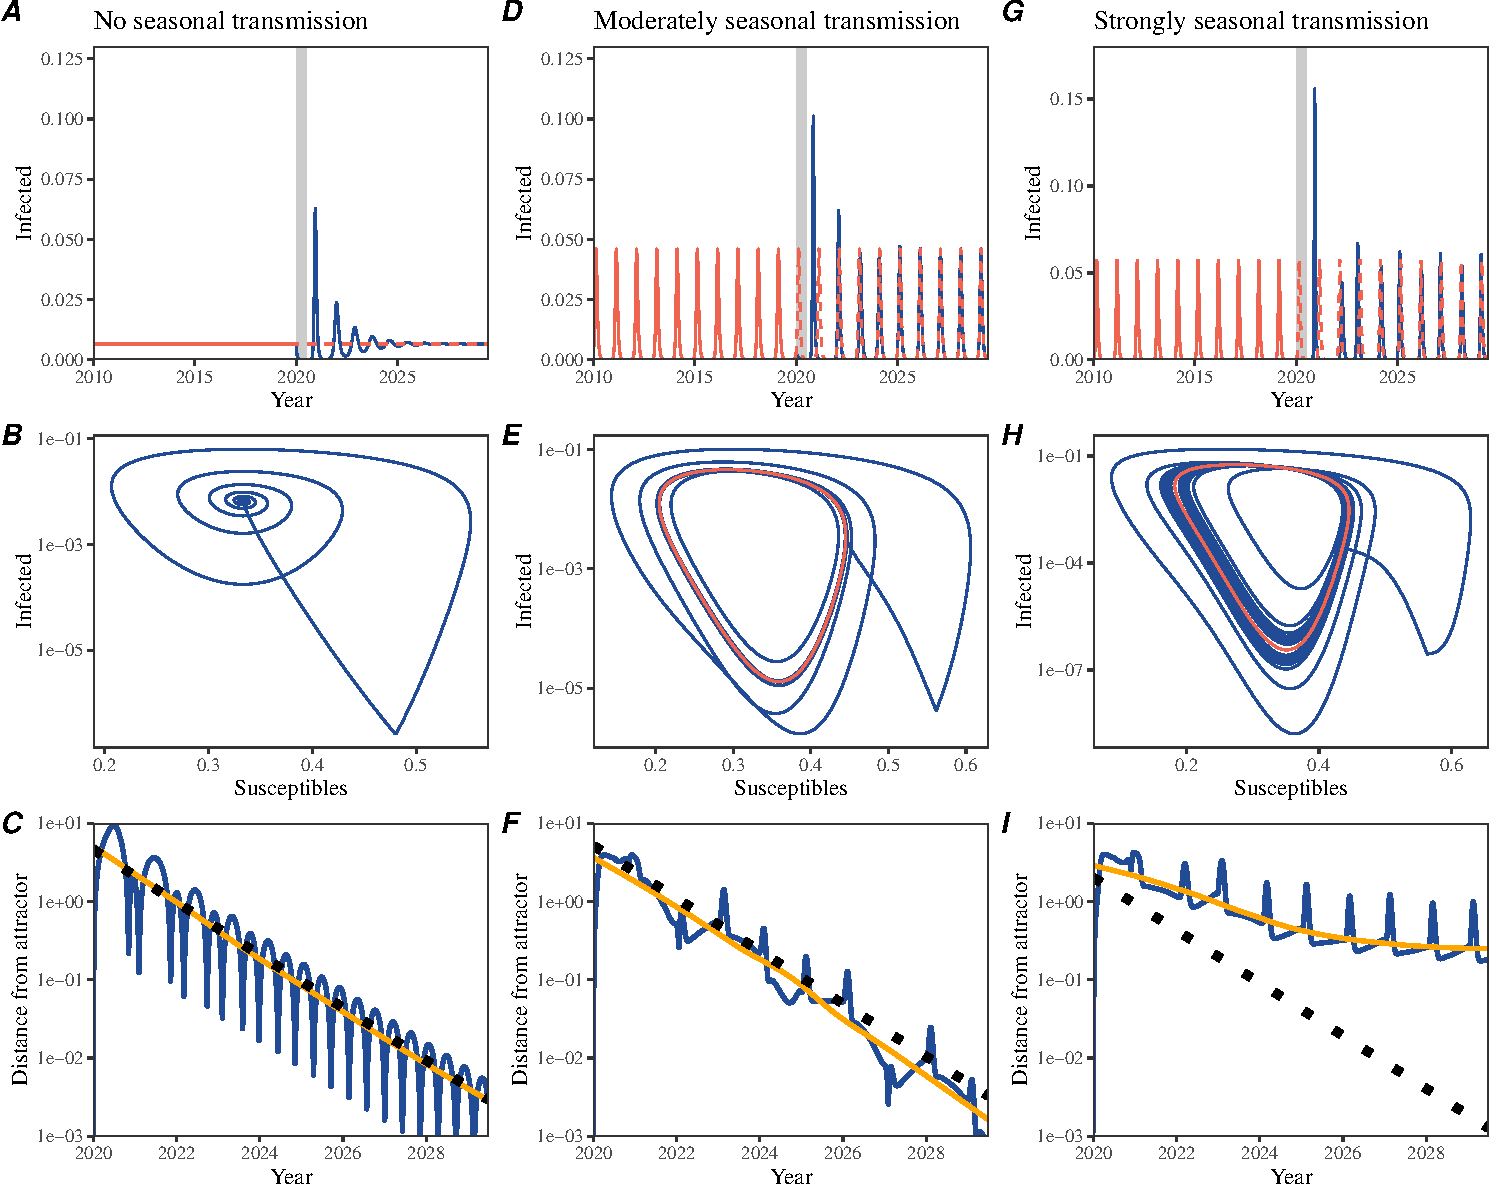
\includegraphics[width=\textwidth]{../figure2/figure2_simple_seas.pdf}
\caption{
\textbf{Impact of seasonal transmission on pathogen resilience.}
(A, D, G) Simulated epidemic trajectories using the SIRS model without seasonal forcing (A), with seasonal forcing of amplitude of 0.2 (D), and with seasonal forcing of amplitude of 0.4 (G).
Red and blue solid lines represent epidemic dynamics before and after interventions are introduced, respectively.
Red dashed lines represent counterfactual epidemic dynamics in the absence of interventions.
Gray regions indicate the duration of interventions.
(B, E, H) Phase plane representation of the time series in panels A, D, and G alongside the corresponding susceptible host dynamics.
Red and blue solid lines represent epidemic trajectories on an SI phase plane before and after interventions are introduced, respectively.
(C, F, I) Changes in logged distance from the attractor over time.
Blue lines represent the logged distance from the attractor.
Orange lines represent the locally estimated scatterplot smoothing (LOESS) fits to the logged distance from the attractor.
Dotted lines show the intrinsic resilience of the seasonally unforced system.
}
\end{figure}

\pagebreak

\begin{figure}[!th]
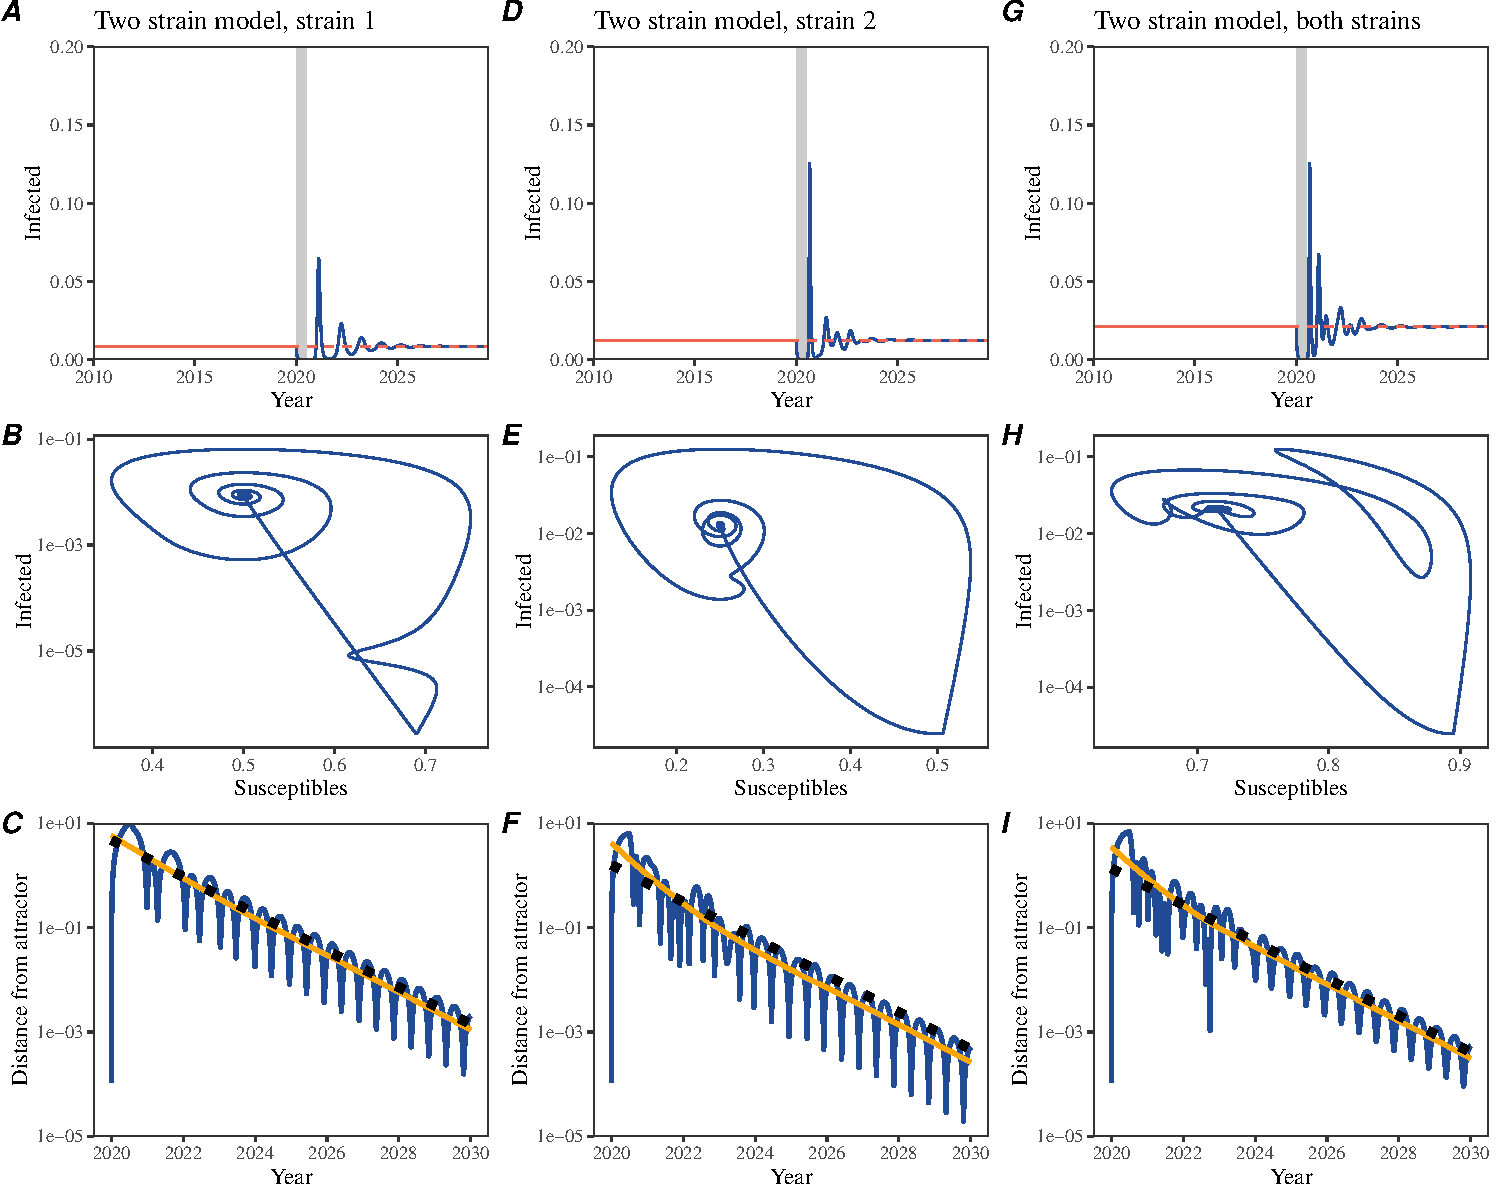
\includegraphics[width=\textwidth]{../figure2/figure2_multi_noseas.pdf}
\caption{
\textbf{A simple method to measure pathogen resilience following pandemic perturbations for a two-strain competition system without seasonal forcing.}
(A, D, G) Simulated epidemic trajectories using a two-strain system without seasonal forcing.
In this model, two strains compete through cross immunity.
Red and blue solid lines represent epidemic dynamics before and after interventions are introduced, respectively.
Red dashed lines represent counterfactual epidemic dynamics in the absence of interventions.
Gray regions indicate the duration of interventions.
(B, E, H) Phase plane representation of the time series in panels A, D, and G alongside the corresponding susceptible host dynamics.
Blue solid lines represent epidemic trajectories on an SI phase plane before and after interventions are introduced, respectively.
(C, F, I) Changes in logged distance from the attractor over time.
Blue lines represent the logged distance from the attractor.
Orange lines represent the locally estimated scatterplot smoothing (LOESS) fits to the logged distance from the attractor.
Dotted lines show the intrinsic resilience of the seasonally unforced system.
}
\end{figure}

\pagebreak

\begin{figure}[!th]
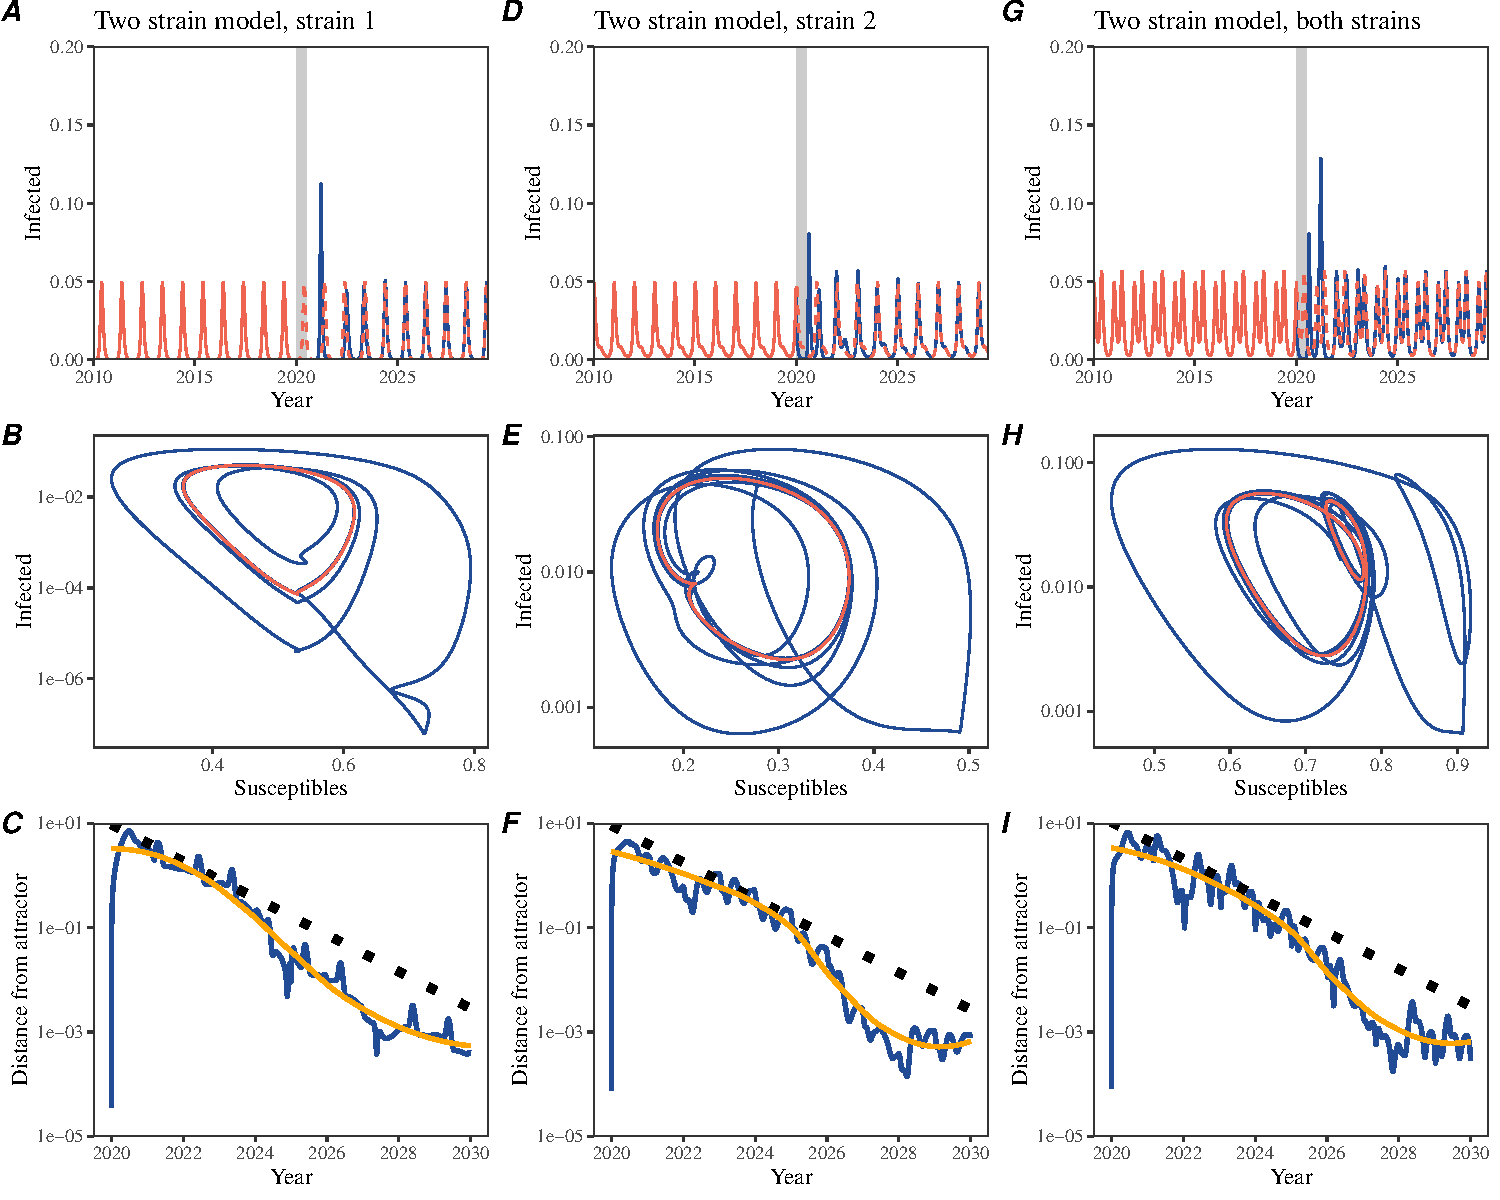
\includegraphics[width=\textwidth]{../figure2/figure2_multi.pdf}
\caption{
\textbf{A simple method to measure pathogen resilience following pandemic perturbations for a two-strain competition system with seasonal forcing.}
(A, D, G) Simulated epidemic trajectories using a two-strain system with seasonal forcing (amplitude of 0.2).
In this model, two strains compete through cross immunity.
Red and blue solid lines represent epidemic dynamics before and after interventions are introduced, respectively.
Red dashed lines represent counterfactual epidemic dynamics in the absence of interventions.
Gray regions indicate the duration of interventions.
(B, E, H) Phase plane representation of the time series in panels A, D, and G alongside the corresponding susceptible host dynamics.
Red and blue solid lines represent epidemic trajectories on an SI phase plane before and after interventions are introduced, respectively.
(C, F, I) Changes in logged distance from the attractor over time.
Blue lines represent the logged distance from the attractor.
Orange lines represent the locally estimated scatterplot smoothing (LOESS) fits to the logged distance from the attractor.
Dotted lines show the intrinsic resilience of the seasonally unforced system.
}
\end{figure}

\pagebreak

\begin{figure}[!th]
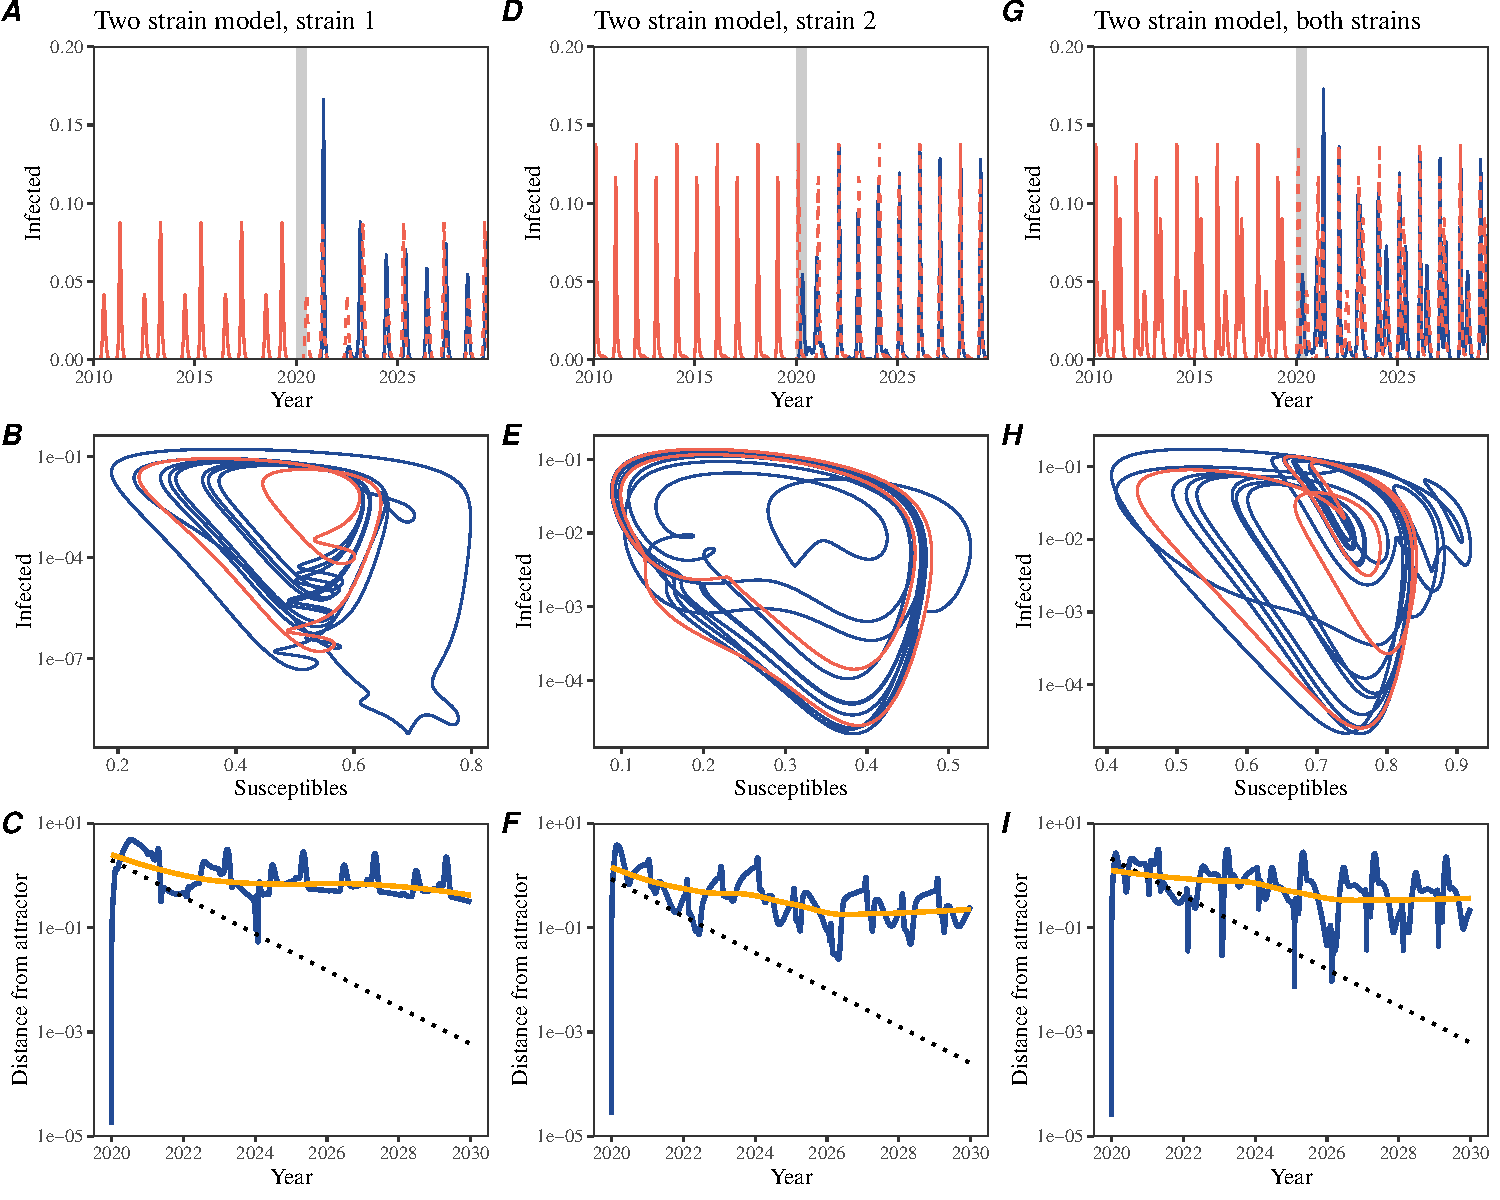
\includegraphics[width=\textwidth]{../figure2/figure2_multi_strong.pdf}
\caption{
\textbf{A simple method to measure pathogen resilience following pandemic perturbations for a multi-strain competition system with strong seasonal forcing.}
(A, D, G) Simulated epidemic trajectories using a two-strain system with seasonal forcing (amplitude of 0.2).
In this model, two strains compete through cross immunity.
Red and blue solid lines represent epidemic dynamics before and after interventions are introduced, respectively.
Red dashed lines represent counterfactual epidemic dynamics in the absence of interventions.
Gray regions indicate the duration of interventions.
(B, E, H) Phase plane representation of the time series in panels A, D, and G alongside the corresponding susceptible host dynamics.
Red and blue solid lines represent epidemic trajectories on an SI phase plane before and after interventions are introduced, respectively.
(C, F, I) Changes in logged distance from the attractor over time.
Blue lines represent the logged distance from the attractor.
Orange lines represent the locally estimated scatterplot smoothing (LOESS) fits to the logged distance from the attractor.
Dotted lines show the intrinsic resilience of the seasonally unforced system.
}
\end{figure}

\pagebreak

\begin{figure}[!th]
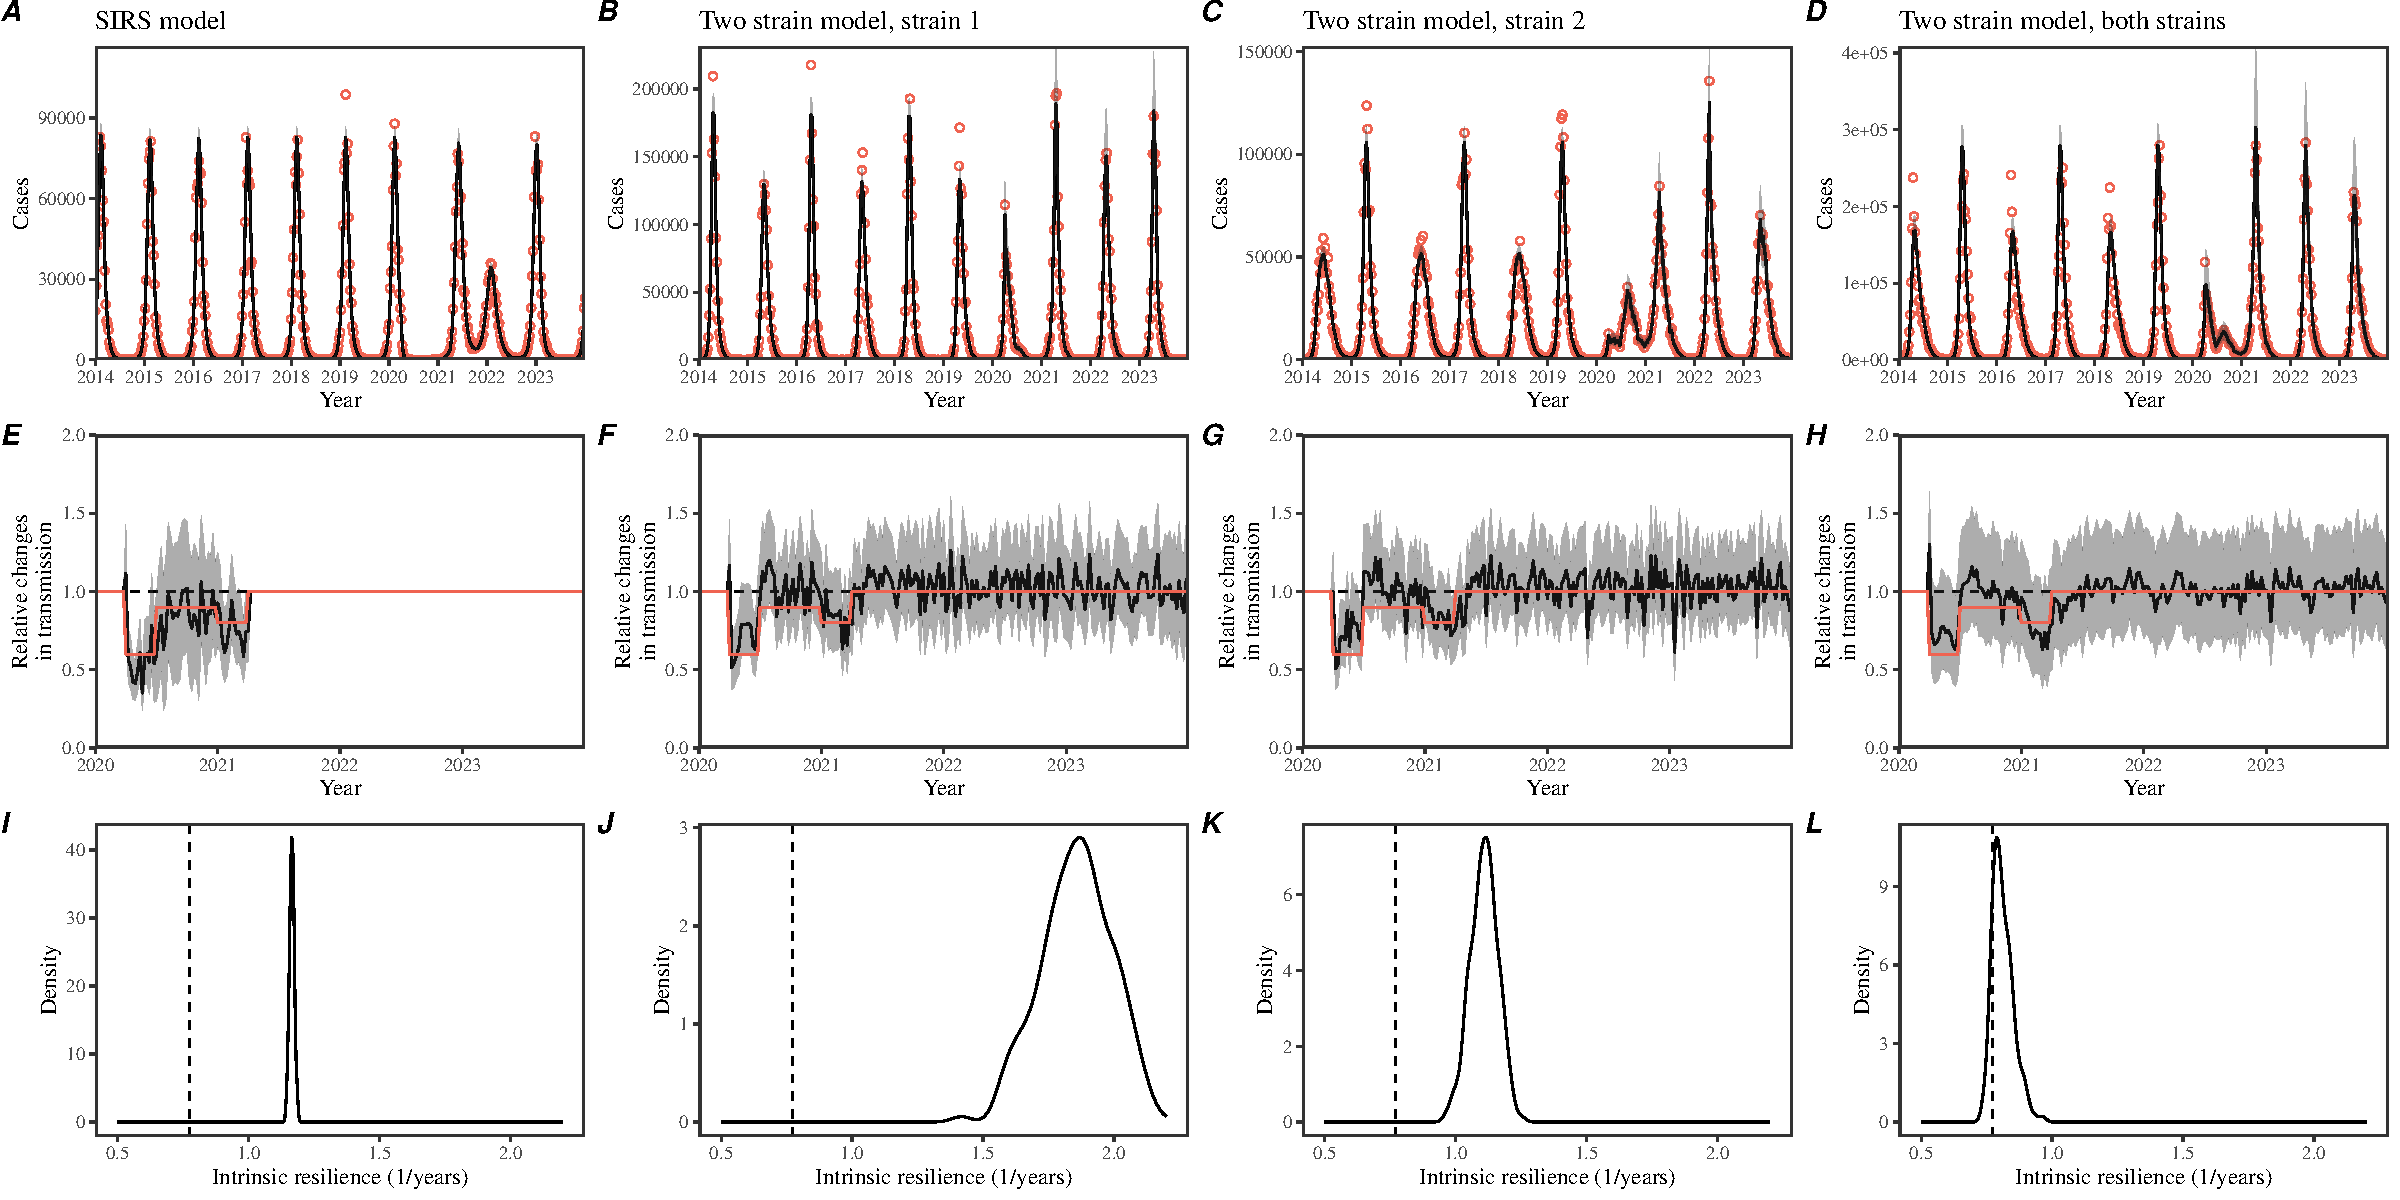
\includegraphics[width=\textwidth]{../figure_fit/figure_fit.pdf}
\caption{
\textbf{Mechanistic model fits to simulated data and inferred intrinsic resilience.}
We simulated discrete time, stochastic epidemic trajectories using a seasonally forced SIRS model (A,E,I) and a seasonally forced two-strain model (B--D, F--H, and J--L) and tested whether we can estimate the intrinsic resilience of the seasonally unforced versions of the model by fitting a mechanistic model (Supplementary Text).
We fitted the same discrete time, one strain, deterministic SIRS model in each scenario.
(A--D) Simulated case time series from corresponding models shown in the title (red) and SIRS model fits (black).
(E--H) Assumed changes in transmission due to pandemic perturbations (red) and estimated time-varying relative transmission rates for the perturbation impact from the SIRS model fits (black).
Solid lines and shaded regions represent fitted posterior median and 95\% credible intervals.
(I--L) Comparisons between the true and estimated intrinsic resilience of the seasonally unforced system.
Vertical lines represent the true intrinsic resilience of the seasonally unforced system.
Density plots represent the posterior distribution of the inferred intrinsic resilience of the seasonally unforced SIRS model using fitted parameters.
}
\end{figure}


\pagebreak

\begin{figure}[!th]
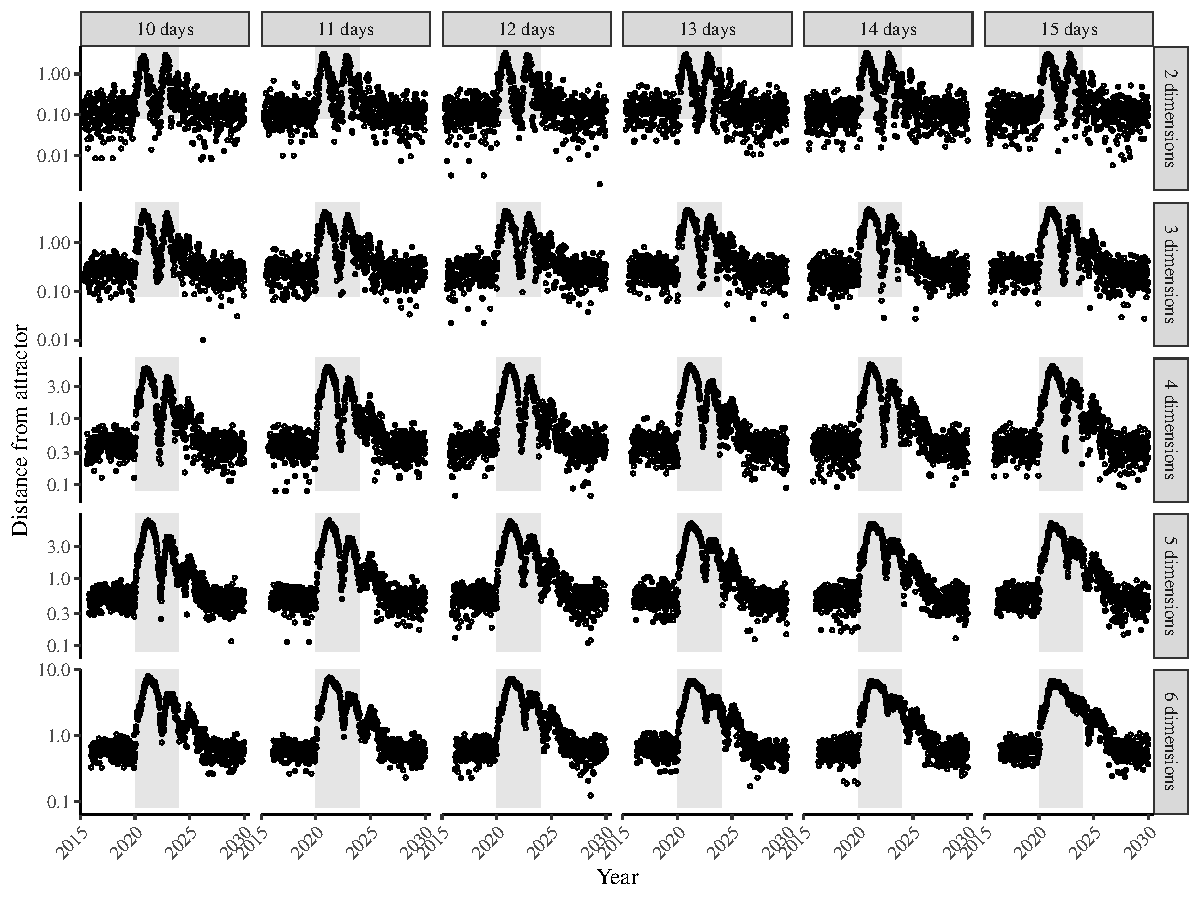
\includegraphics[width=\textwidth]{../figure3/figure3_sens.pdf}
\caption{
\textbf{Sensitivity of the distance from the attractor to choice of embedding lags and dimensions.}
Sensitivity analysis for the distance-from-attractor time series shown in Figure 3E in the main text by varying the embedding lag between 10--15 days and embedding dimensions between 2--6 dimensions.
The gray region represents the assumed period of pandemic perturbation.
}
\end{figure}

\pagebreak

\begin{figure}[!th]
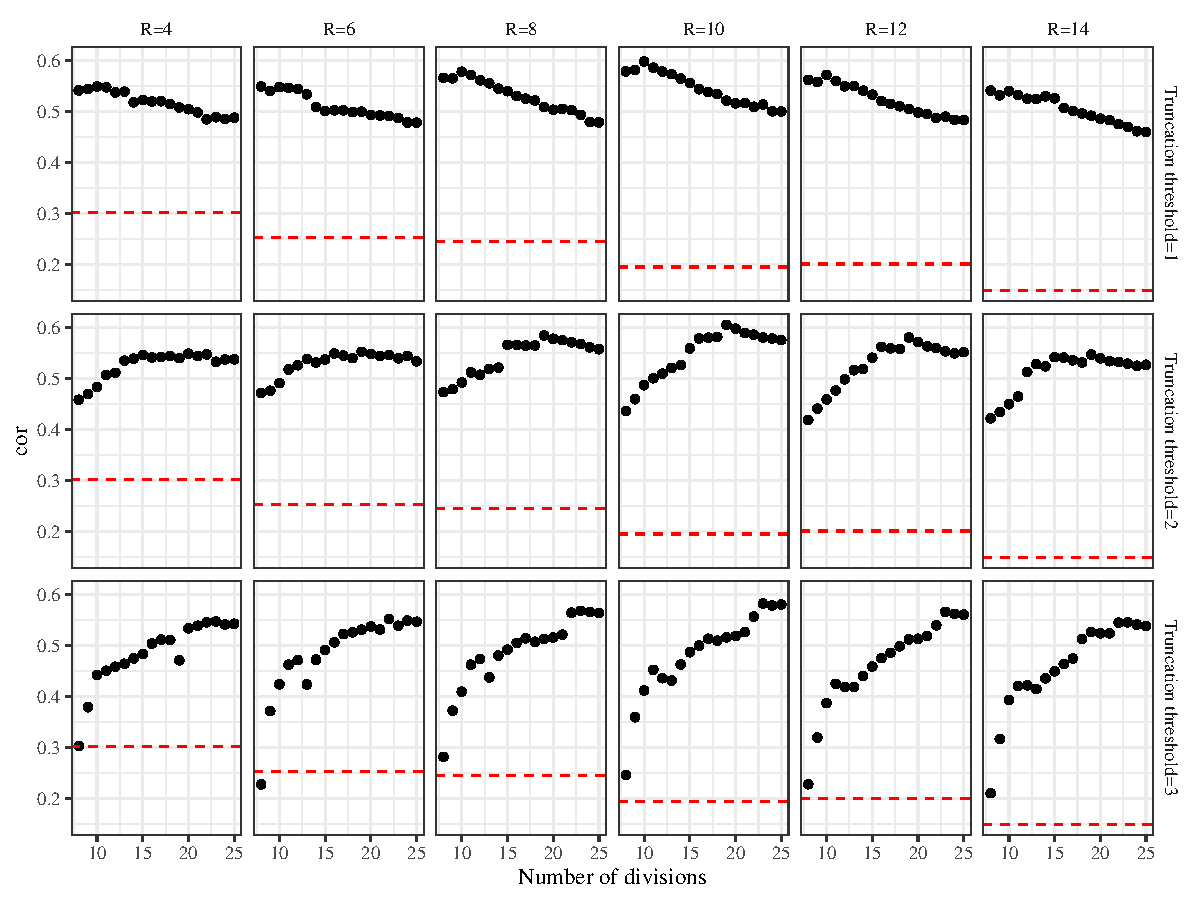
\includegraphics[width=\textwidth]{../figure_analysis_random/figure_analysis_random.pdf}
\caption{
\textbf{Impact of fitting window selection on the estimation of empirical resilience.}
We simulated 500 epidemics of a stochastic SIRS model with randomly drawn parameters and randomly generated pandemic perturbations (Supplementary Text).
For each simulation, we varied the false nearest neighbor threshold $R$ for reconstructing the empirical attractor as well as the parameters for regression window selection (i.e., the truncation threshold $a$ and the number of divisions $K$).
Each point represents the resulting correlation coefficient between empirical and intrinsic resilience estimates for a given scenario.
Dashed lines represent the correlation coefficient between empirical and intrinsic resilience estimates for the naive approach that fits a linear regression on a log scale, starting from the maximum distance until the end of the time series.
}
\end{figure}

\pagebreak

\begin{figure}[!th]
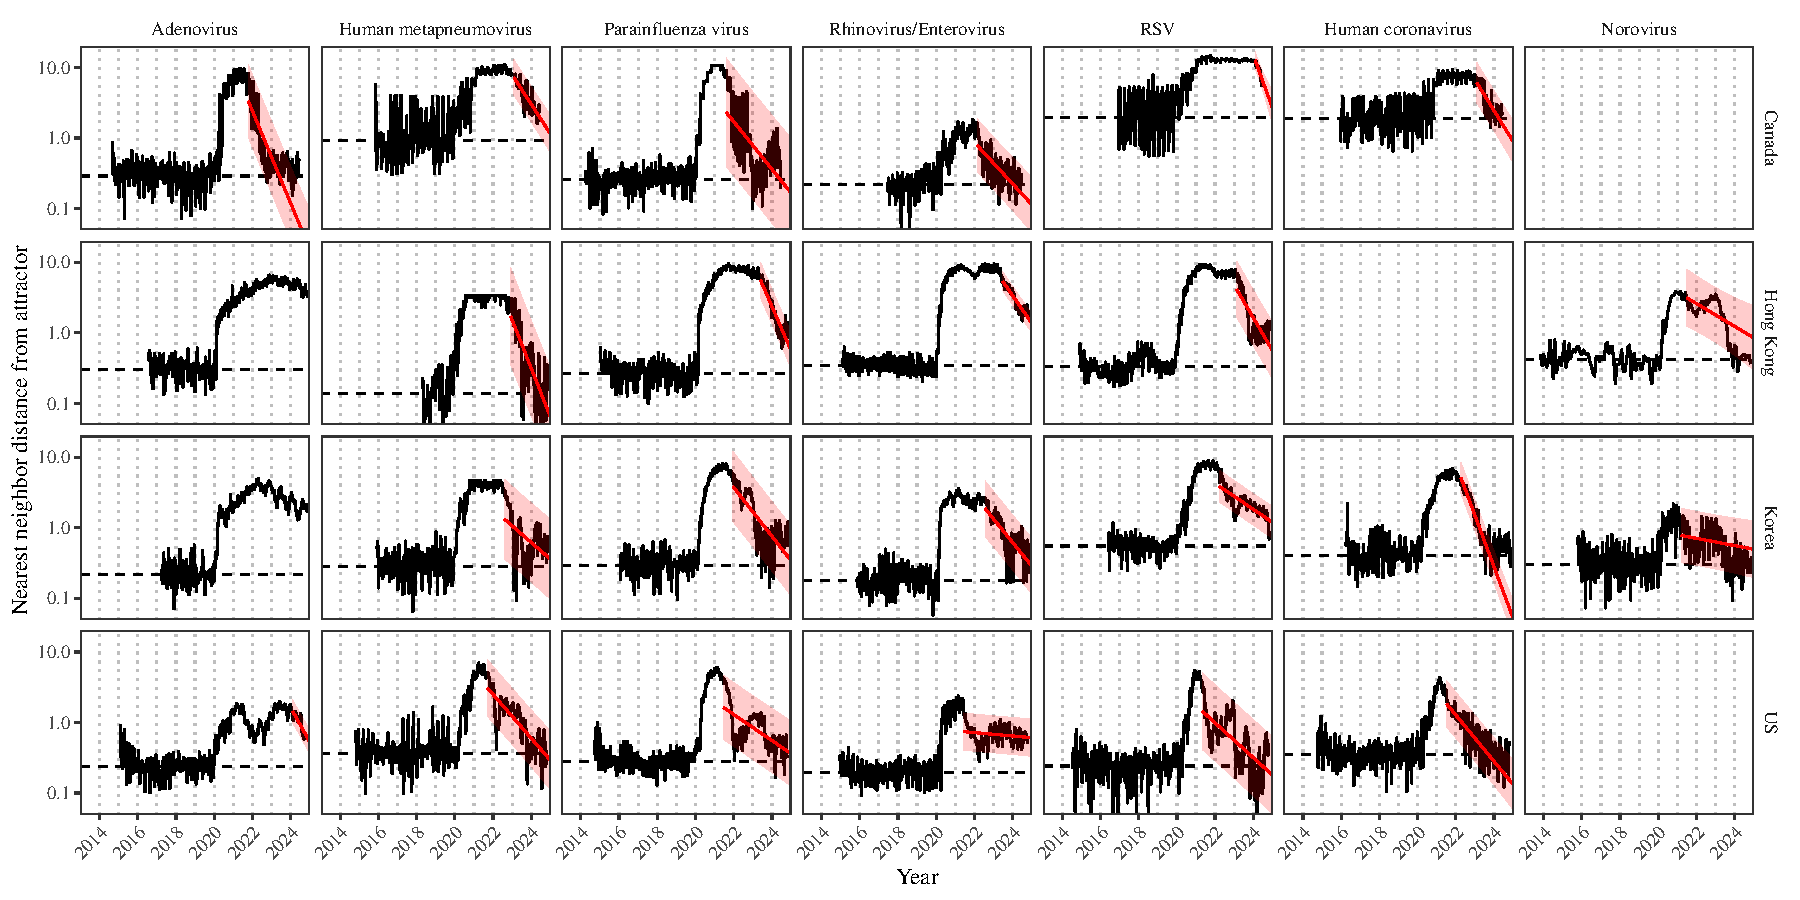
\includegraphics[width=\textwidth]{../figure4/figure4_dist_auto.pdf}
\caption{
\textbf{Estimated time series of distance from the attractor for each pathogen and corresponding linear regression fits using automated window selection criterion across Canada, Hong Kong, Korea, and the US.}
Black lines represent the estimated distance from the attractor.
Red lines and shaded regions represent the linear regression fits and corresponding 95\% confidence intervals.
Dashed lines represent the average of the pre-pandemic nearest neighbor distances.
}
\end{figure}

\pagebreak

\begin{figure}[!th]
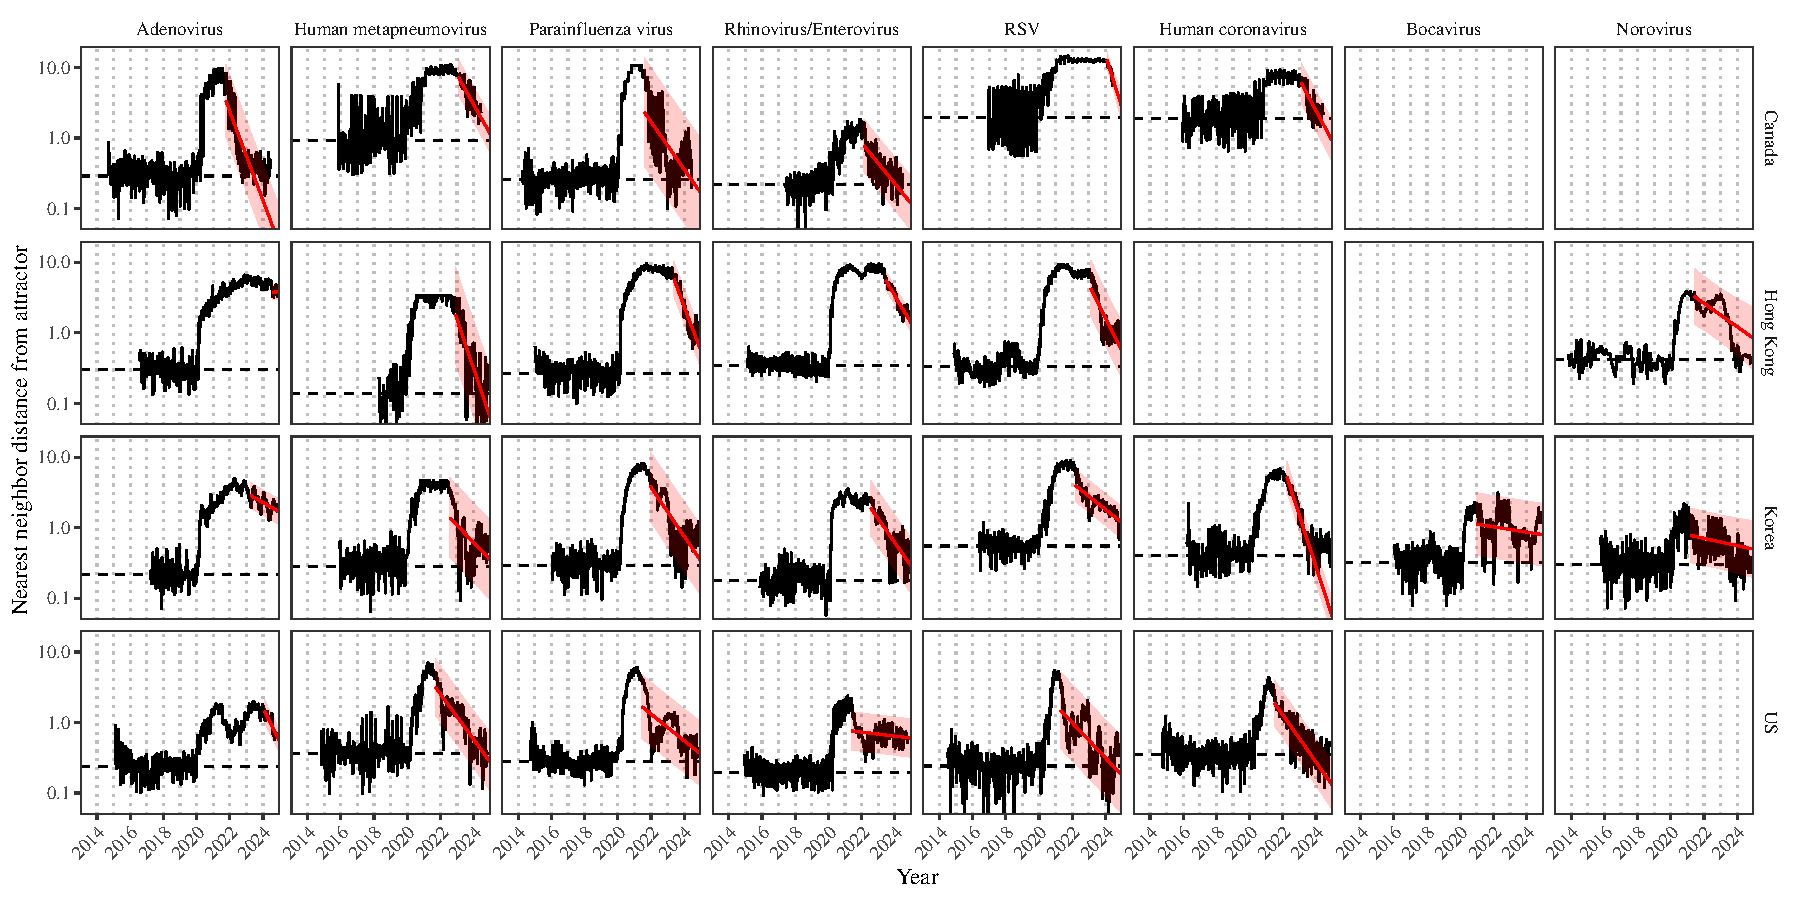
\includegraphics[width=\textwidth]{../figure4/figure4_dist.pdf}
\caption{
\textbf{Estimated time series of distance from the attractor for each pathogen and corresponding linear regression fits across Canada, Hong Kong, Korea, and the US, including ad-hoc regression window selection.}
We used ad-hoc regression windows for norovirus in Hong Kong and Korea and rhinovirus/enterovirus in the US.
Black lines represent the estimated distance from the attractor.
Red lines and shaded regions represent the linear regression fits and corresponding 95\% confidence intervals.
Dashed lines represent the average of the pre-pandemic nearest neighbor distances.
}
\end{figure}

\pagebreak

\begin{figure}[!th]
\begin{center}
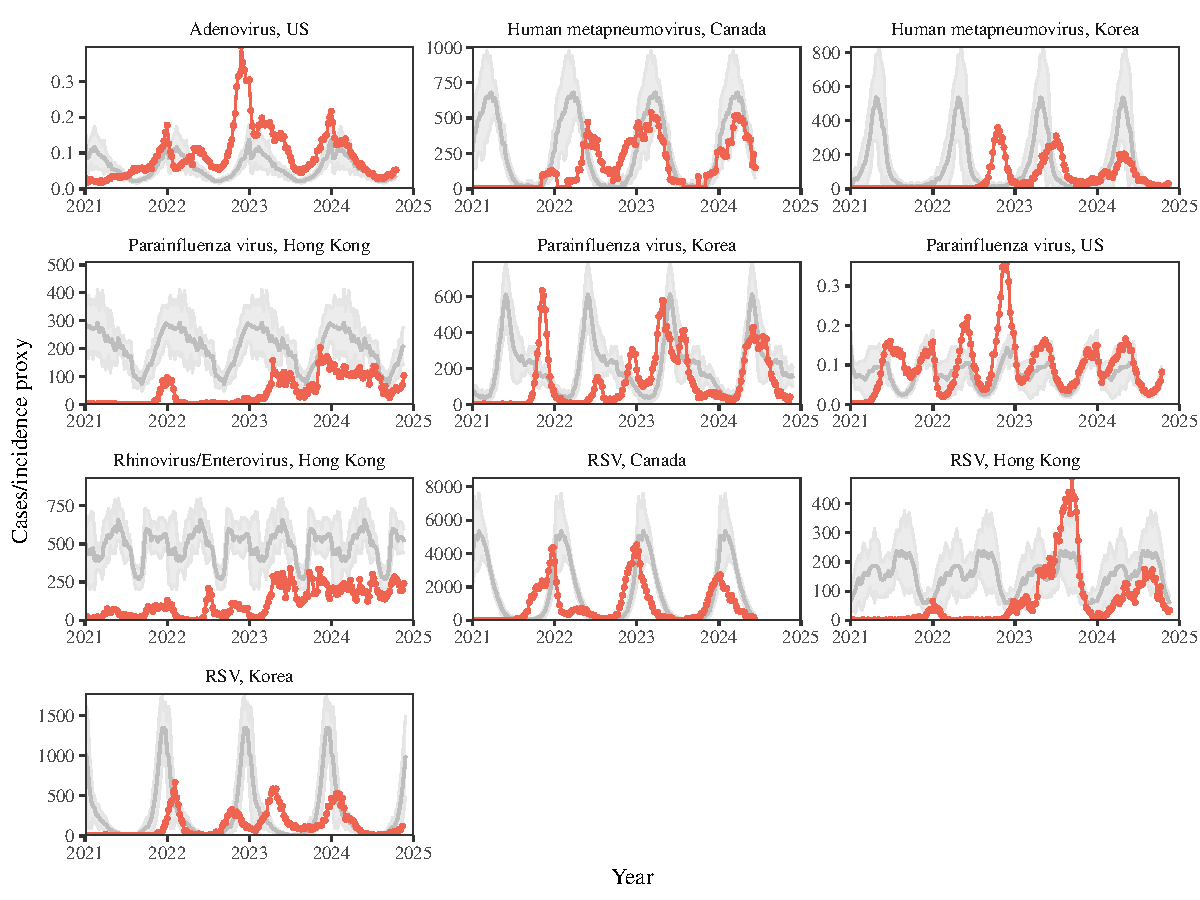
\includegraphics[width=\textwidth]{../figure4/figure4_noreturn.pdf}
\caption{
\textbf{Observed dynamics for pathogen that are predicted to return after the end of 2024.}
Red points and lines represent data before 2020.
Gray lines and shaded regions represent the mean seasonal patterns and corresponding 95\% confidence intervals around the mean, previously shown in Figure 1.
}
\end{center}
\end{figure}


\pagebreak

\begin{figure}[!th]
\begin{center}
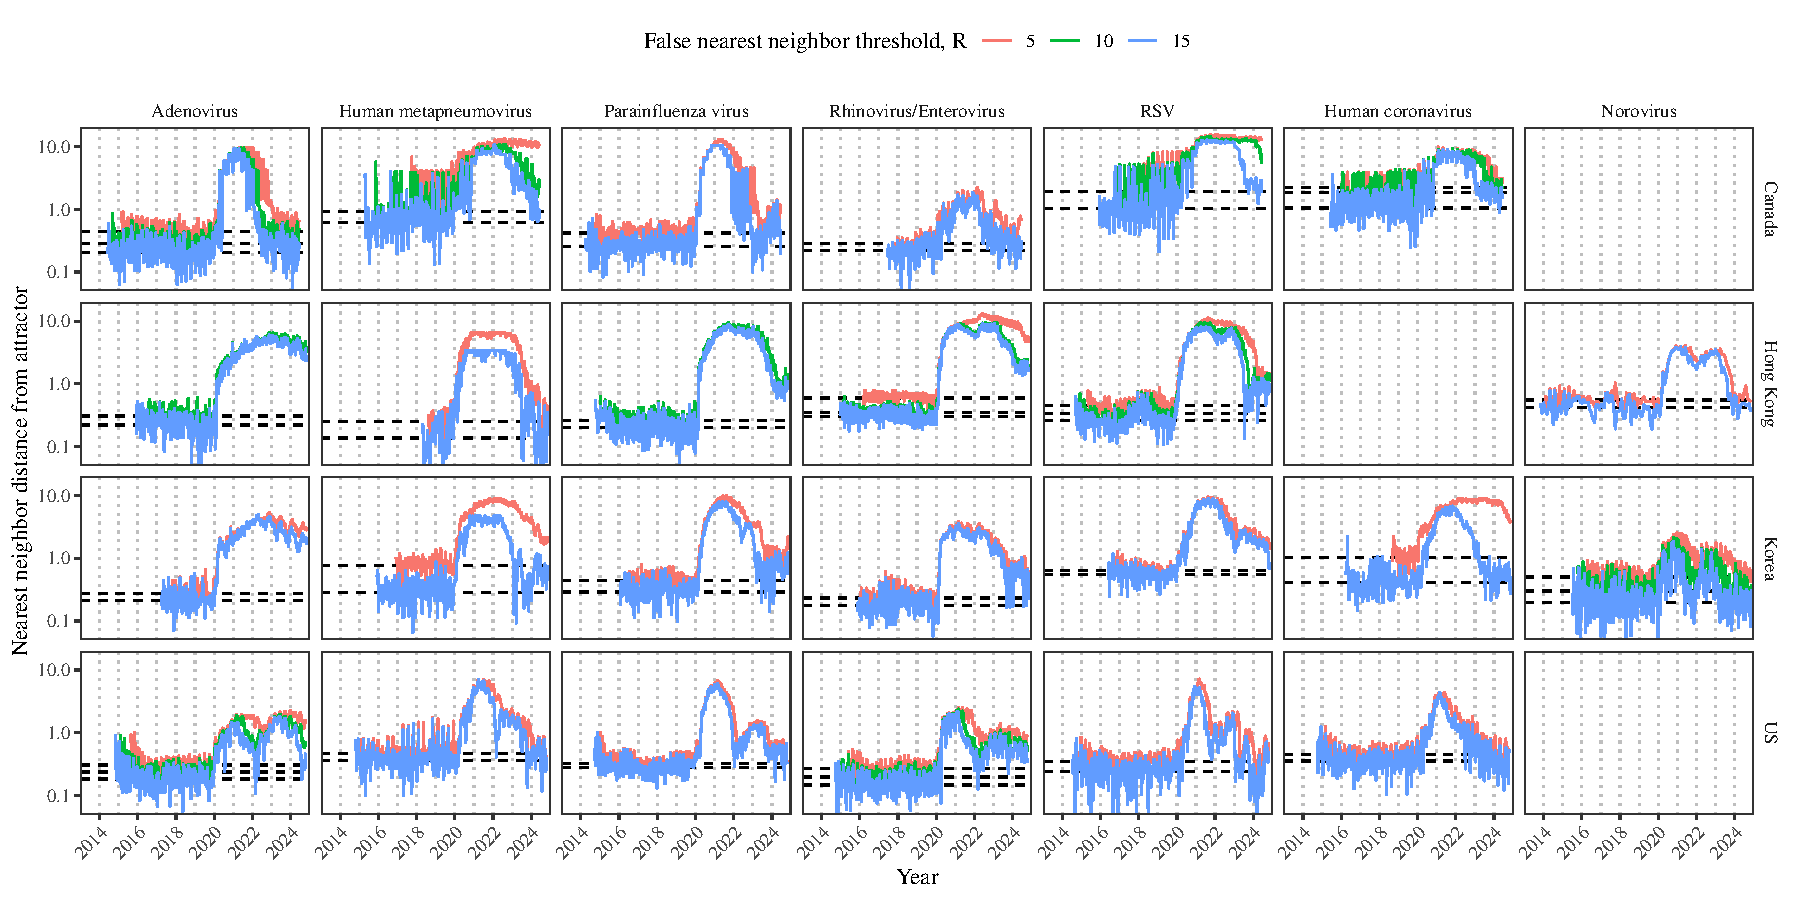
\includegraphics[width=\textwidth]{../figure4_R/figure4_dist_R.pdf}
\caption{
\textbf{Estimated time series of distance from the attractor for each pathogen across different choices about false nearest neighbor threshold values.}
Using higher threshold values for the false nearest neighbor approach gives lower embedding dimensions.
Colored lines represent the estimated distance from the attractor for different threshold values.
}
\end{center}
\end{figure}

\pagebreak

\begin{figure}[!th]
\begin{center}
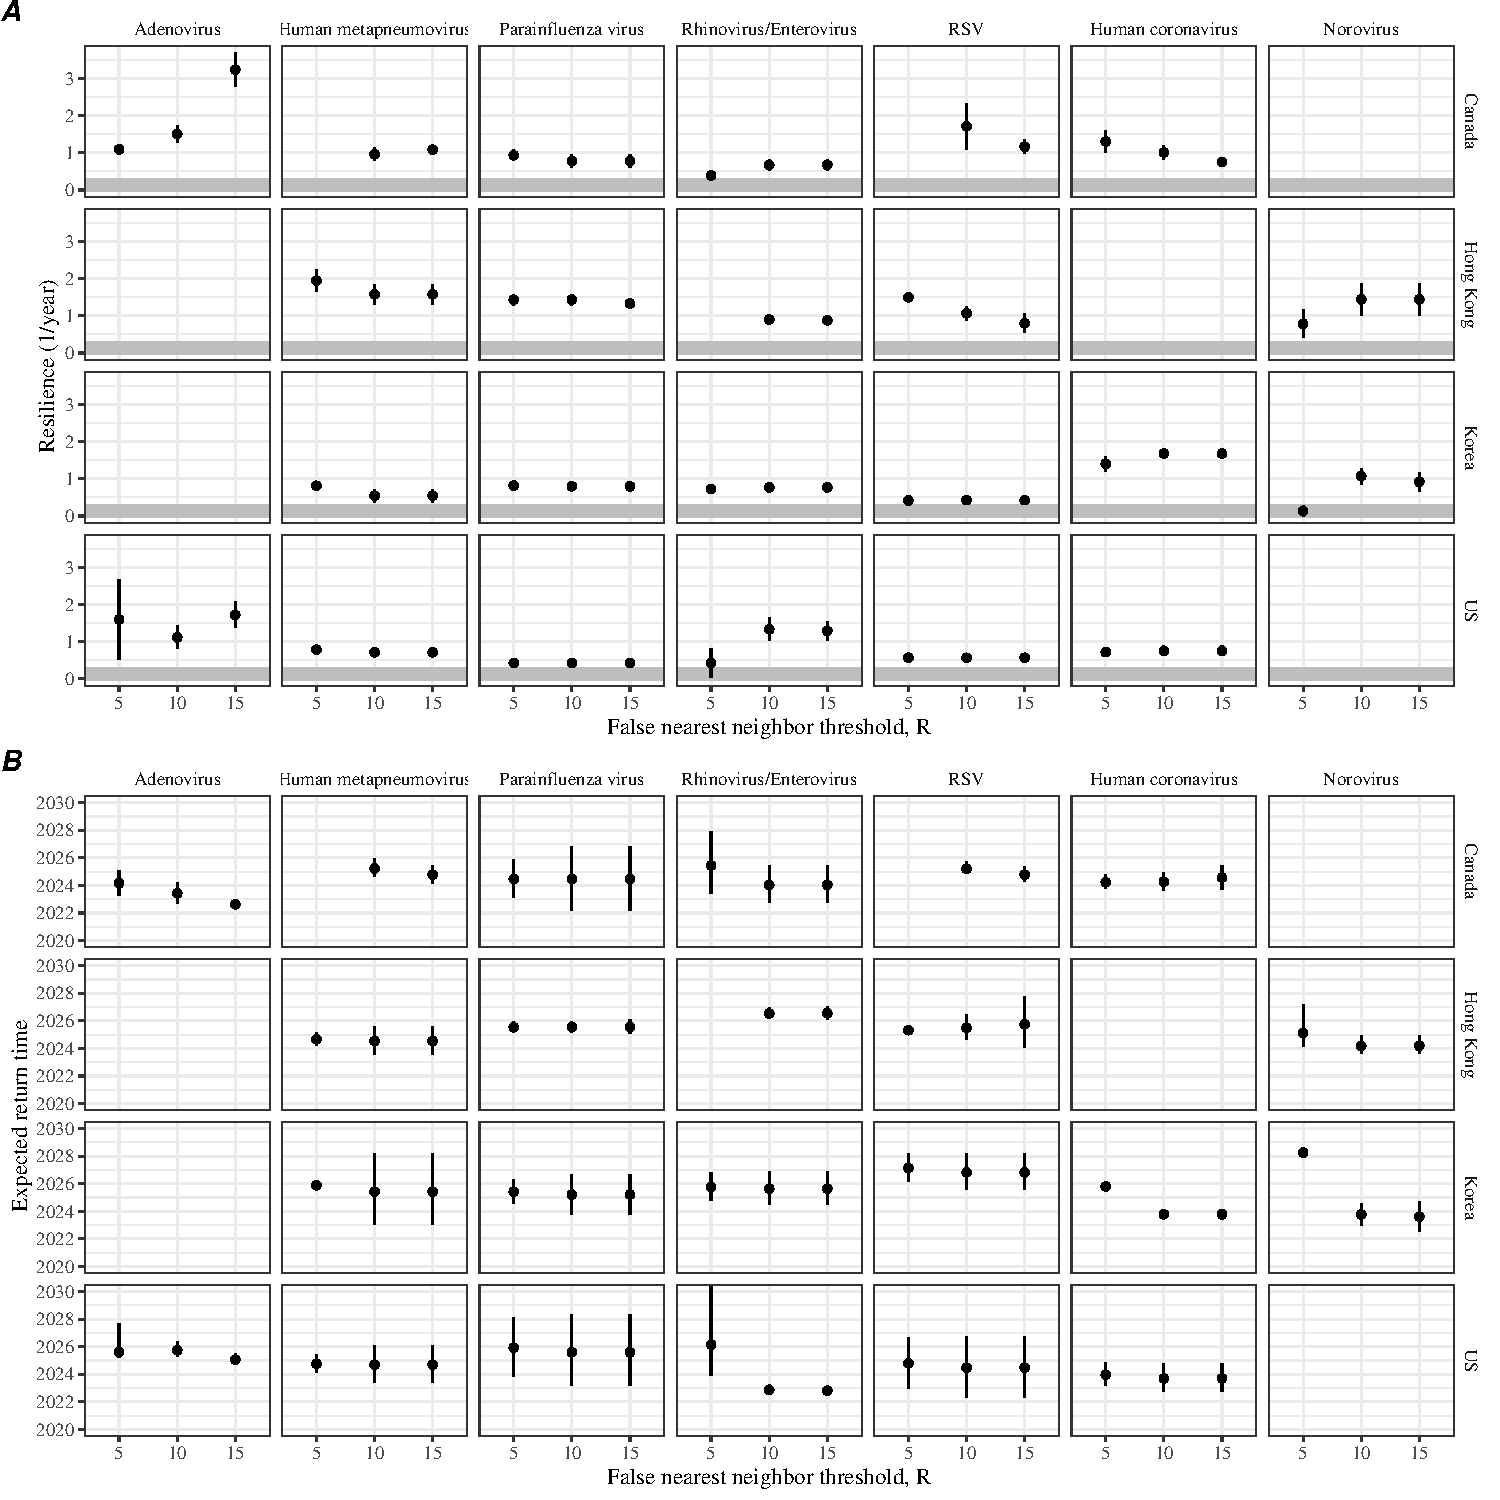
\includegraphics[width=0.9\textwidth]{../figure4_R/figure4_R.pdf}
\caption{
\textbf{Summary of resilience estimates and predictions for return time across different choices about false nearest neighbor threshold values.}
The automated window selection method was used for all scenarios to estimate pathogen resilience, except for norovirus in Hong Kong and Korea and rhinovirus/enterovirus in the US.
We used the same ad-hoc regression windows for norovirus in Hong Kong and Korea and rhinovirus/enterovirus in the US as we did in the main analysis.
(A) Estimated pathogen resilience.
The gray horizontal line represents the intrinsic resilience of pre-vaccination measles dynamics.
(B) Predicted timing of when each pathogen will return to their pre-pandemic cycles.
The dashed line in panel B indicates the end of 2024.
Error bars represent 95\% confidence intervals.
}
\end{center}
\end{figure}

\pagebreak

\begin{figure}[!th]
\begin{center}
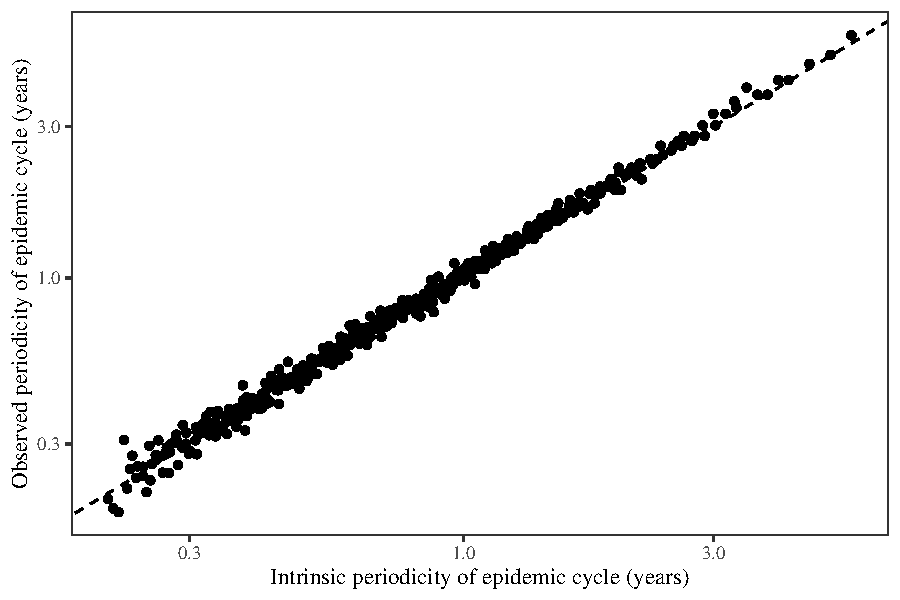
\includegraphics[width=\textwidth]{../figure6/figure_persistence_noise_period.pdf}
\caption{
\textbf{Comparison between the observed and intrisic periodicity of the epidemic cycle of the seasonally unforced SIRS model.}
The observed periodicity of the epidemic corresponds to the periodicity at which maximum spectral density occurs.
The intrinsic periodicity of the epidemic corresponds to $2 \pi/\mathrm{Im}(\lambda)$, where $\mathrm{Im}(\lambda)$ is the imaginary part of the eigenvalue.
}
\end{center}
\end{figure}

\pagebreak

\begin{figure}[!th]
\begin{center}
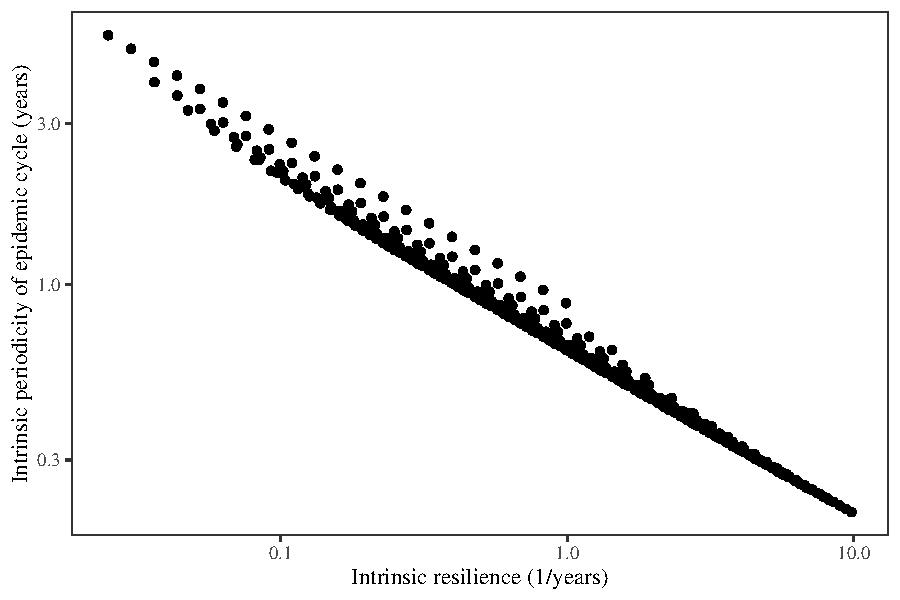
\includegraphics[width=\textwidth]{../figure6/figure_persistence_noise_resilience_period.pdf}
\caption{
\textbf{Comparison between the intrisic resilience and periodicity of the epidemic cycle of the seasonally unforced SIRS model.}
The intrinsic resilience of the epidemic corresponds to the negative of the real value of the eigenvalue $-\mathrm{Re}(\lambda)$.
The intrinsic periodicity of the epidemic corresponds to $2 \pi/\mathrm{Im}(\lambda)$, where $\mathrm{Im}(\lambda)$ is the imaginary part of the eigenvalue.
}
\end{center}
\end{figure}


\pagebreak

\begin{figure}[!th]
\begin{center}
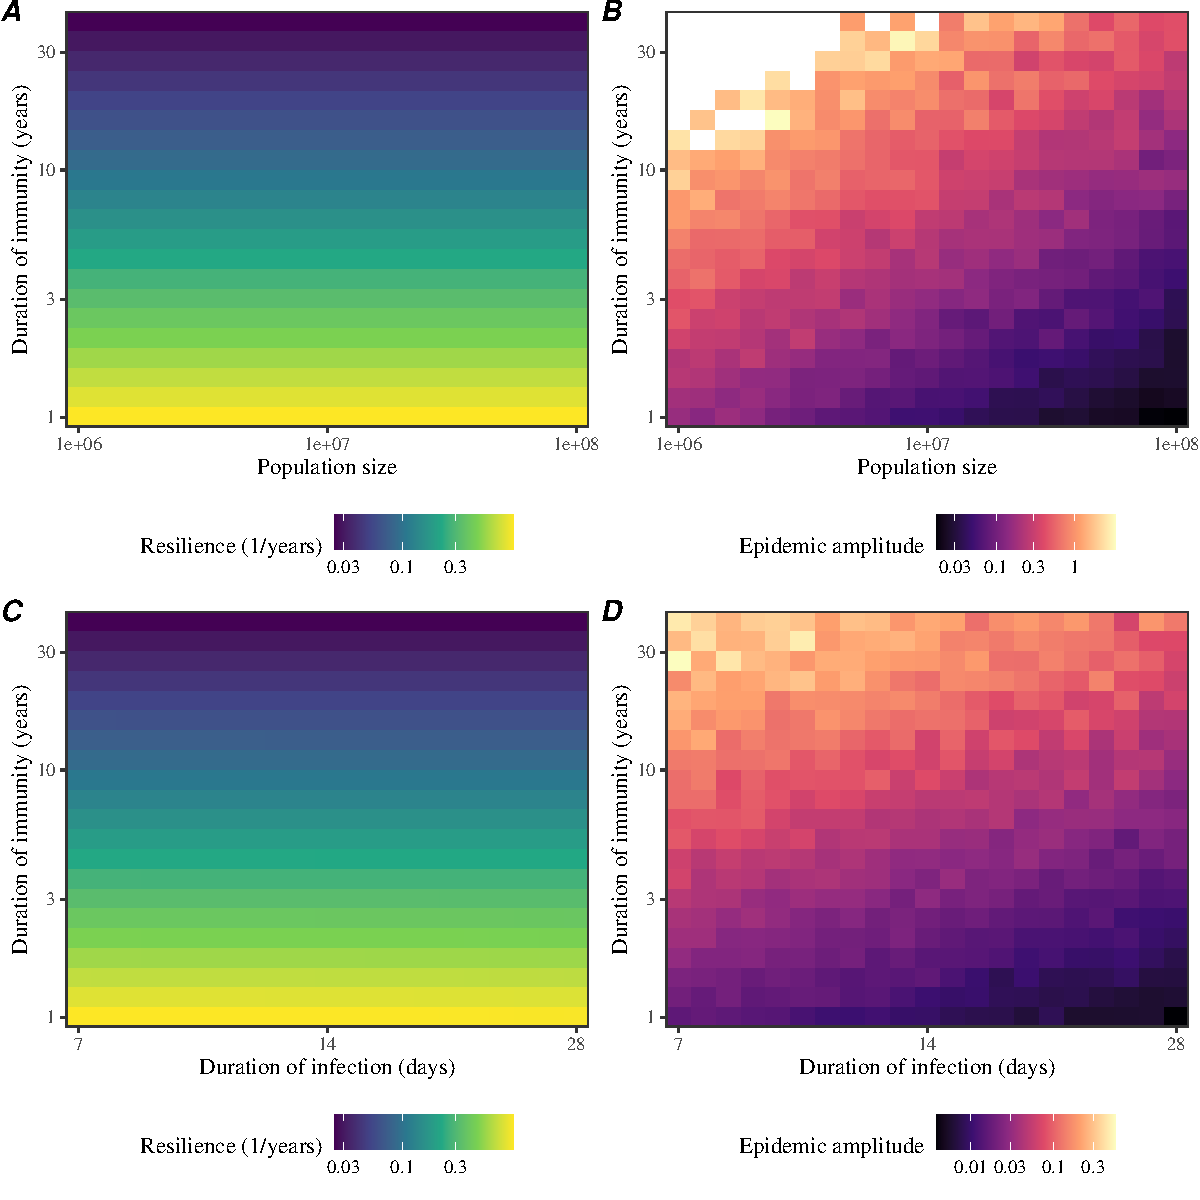
\includegraphics[width=\textwidth]{../figure6/figure_persistence_noise_popgamma.pdf}
\caption{
\textbf{Impact of population size and the average duration of infection of a host-pathogen system on its sensitivity to stochastic perturbations.}
(A) Intrinsic resilience of a system as a function of population size and the average duration of immunity.
(B) Epidemic amplitude as a function of population size and the average duration of immunity.
(C) Intrinsic resilience of a system as a function of the average duration of infection and immunity.
(D) Epidemic amplitude as a function of the average duration of infection and immunity.
The epidemic amplitude corresponds to $(\max I - \min I)/(2 \bar{I})$, where $\bar{I}$ represents the mean prevalence.
}
\end{center}
\end{figure}

\pagebreak

\begin{figure}[!th]
\begin{center}
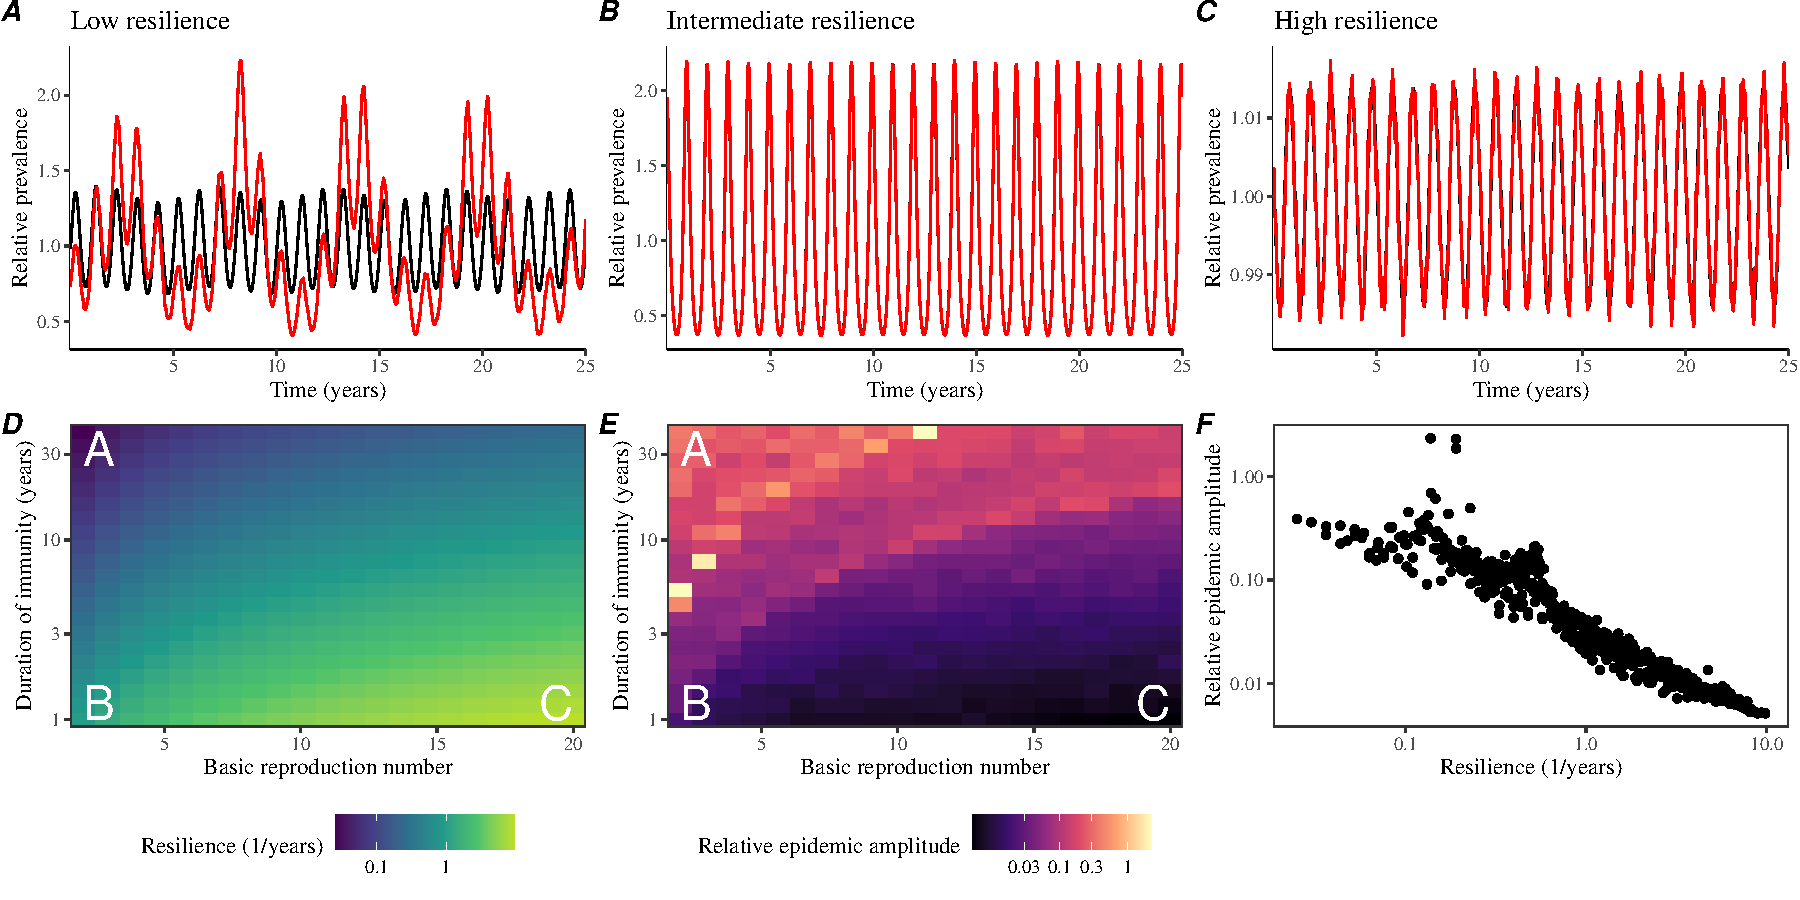
\includegraphics[width=\textwidth]{../figure6/figure_persistence_noise_cycle.pdf}
\caption{
\textbf{Linking resilience of a host-pathogen system to its sensitivity to stochastic perturbations for the seasonally forced SIRS model.}
(A--C) Epidemic trajectories of a stochastic SIRS model with demographic stochasticity across three different resilience values: low, intermediate, and high.
The relative prevalence was calculated by dividing infection prevalence by its mean value.
Black lines represent deterministic epidemic trajectories.
Red lines represent stochastic epidemic trajectories.
(D) The intrinsic resilience of the seasonally unforced system as a function of the basic reproduction number $\mathcal R_0$ and the duration of immunity.
(E) The relative epidemic amplitude, a measure of sensitivity to stochastic perturbations, as a function of the basic reproduction number $\mathcal R_0$ and the duration of immunity.
To calculate the relative epidemic amplitude, we first take the relative difference in infection prevalence between stochastic and deterministic trajectories: $\epsilon = (\tsub{I}{stoch}-\tsub{I}{det})/\tsub{I}{det}$. 
Then, we calculate the difference between maximum and minimum of the relative difference and divide by half: $(\max \epsilon - \min \epsilon)/2$.
Labels A--C in panels D and E correspond to scenarios shown in panels A--C.
(F) The relationship between pathogen resilience and relative epidemic amplitude.
}
\end{center}
\end{figure}

\pagebreak

\begin{figure}[!th]
\begin{center}
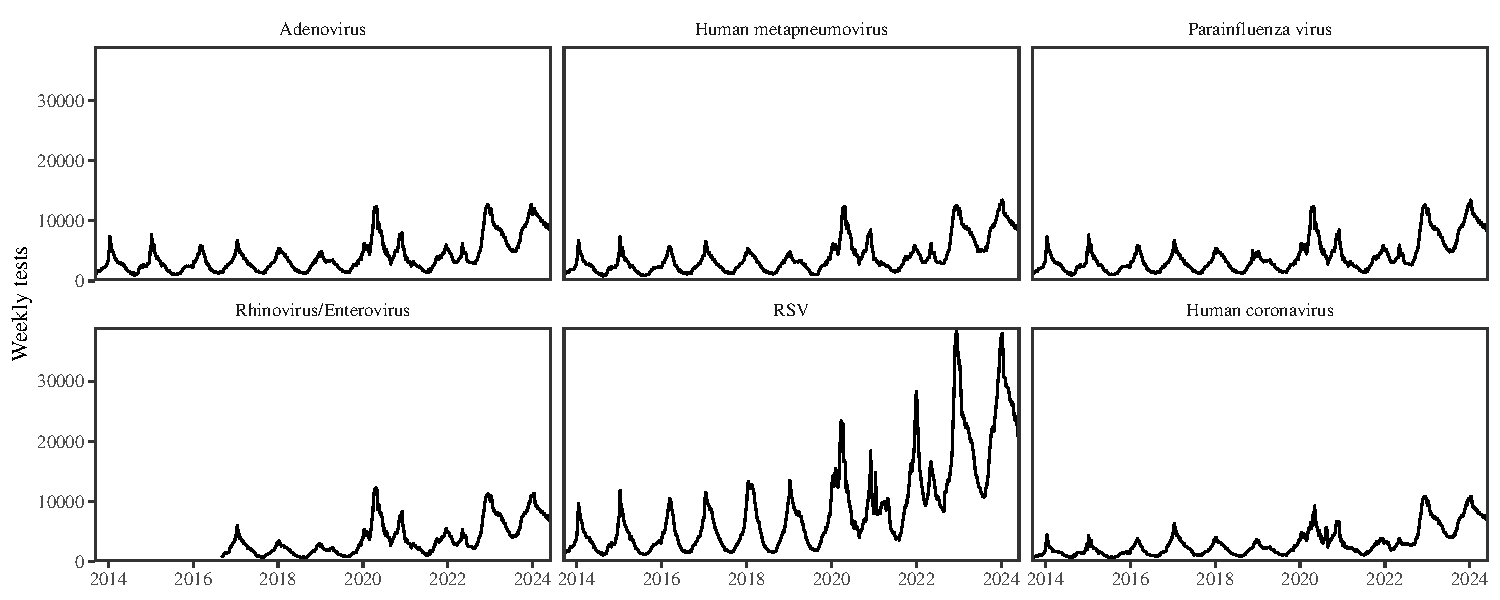
\includegraphics[width=\textwidth]{../figure_test/figure_test_canada.pdf}
\caption{
\textbf{Testing patterns for respiratory pathogens in Canada.}
}
\end{center}
\end{figure}

\pagebreak

\begin{figure}[!th]
\begin{center}
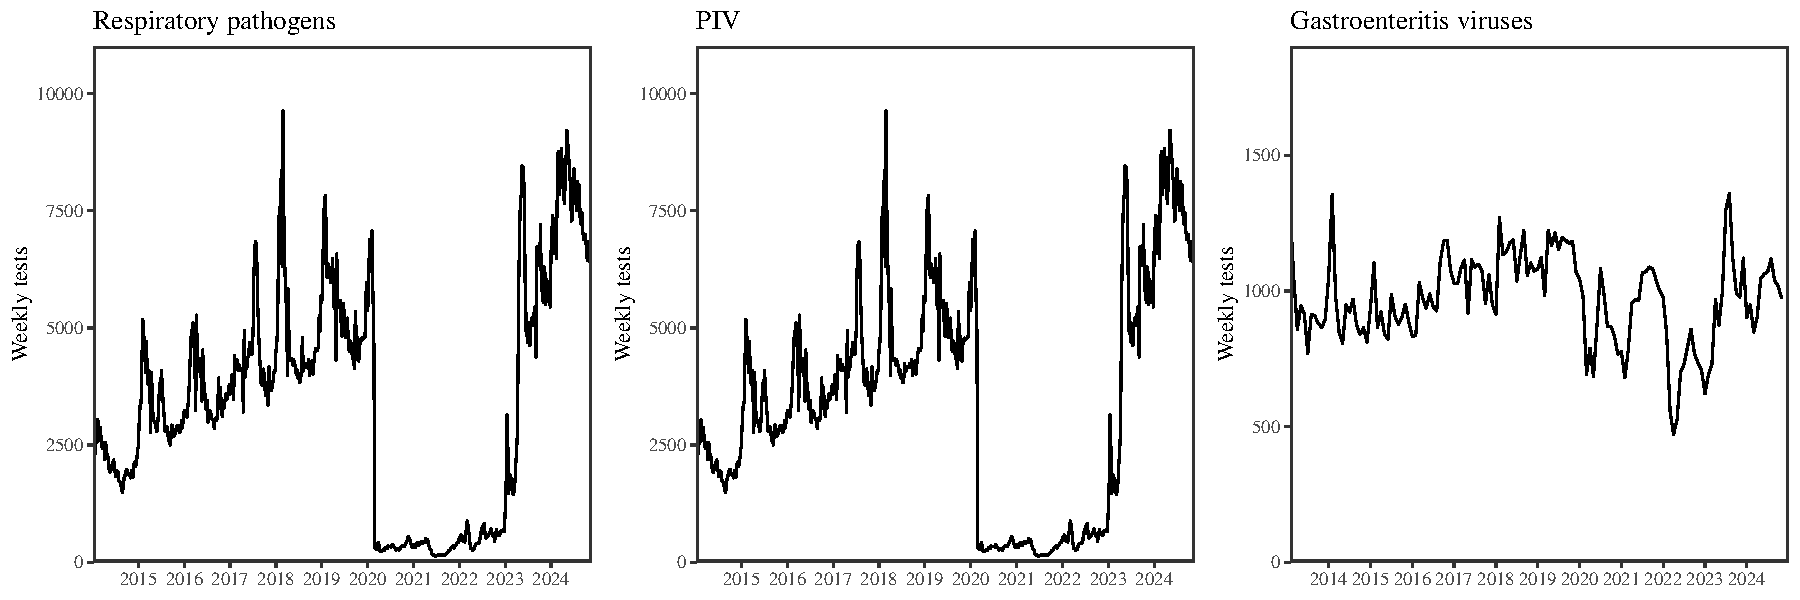
\includegraphics[width=\textwidth]{../figure_test/figure_test_hongkong.pdf}
\caption{
\textbf{Testing patterns for respiratory pathogens, PIV, and gastroenteritis viruses in Hong Kong.}
}
\end{center}
\end{figure}


\pagebreak

\begin{figure}[!th]
\begin{center}
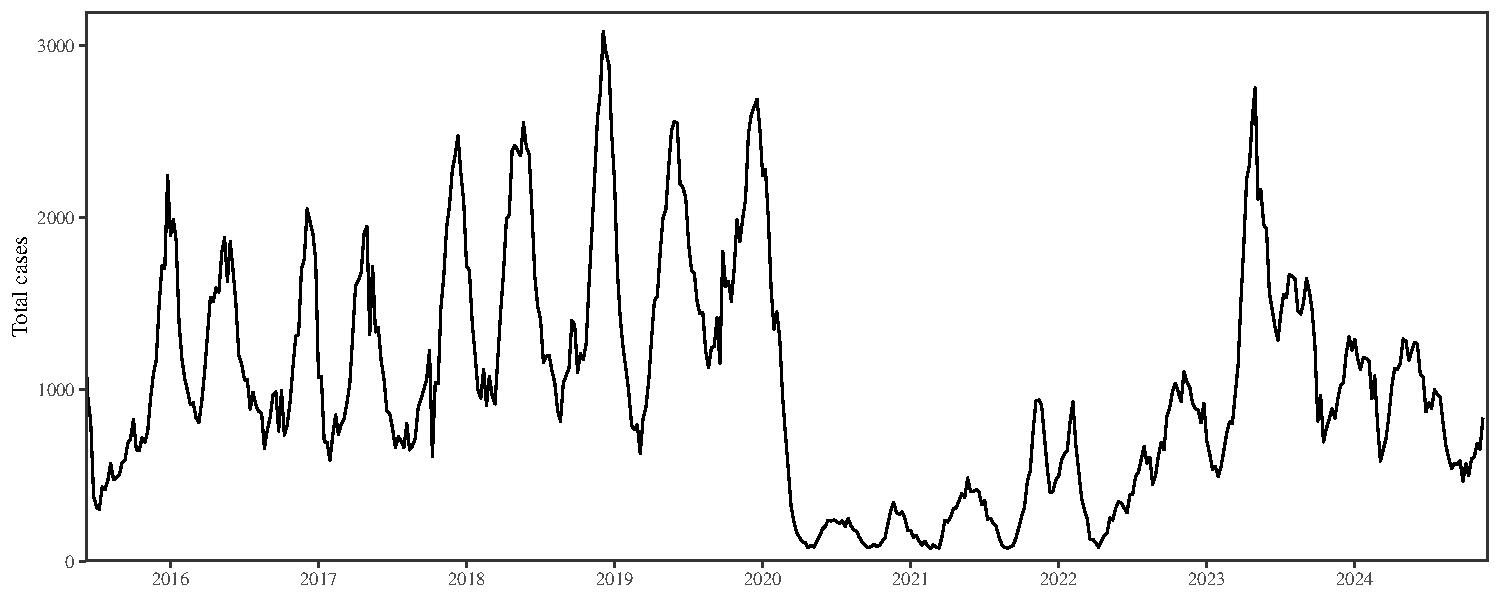
\includegraphics[width=\textwidth]{../figure_test/figure_test_korea.pdf}
\caption{
\textbf{Total number of reported respiratory infection cases in Korea.}
}
\end{center}
\end{figure}

\pagebreak

\begin{figure}[!th]
\begin{center}
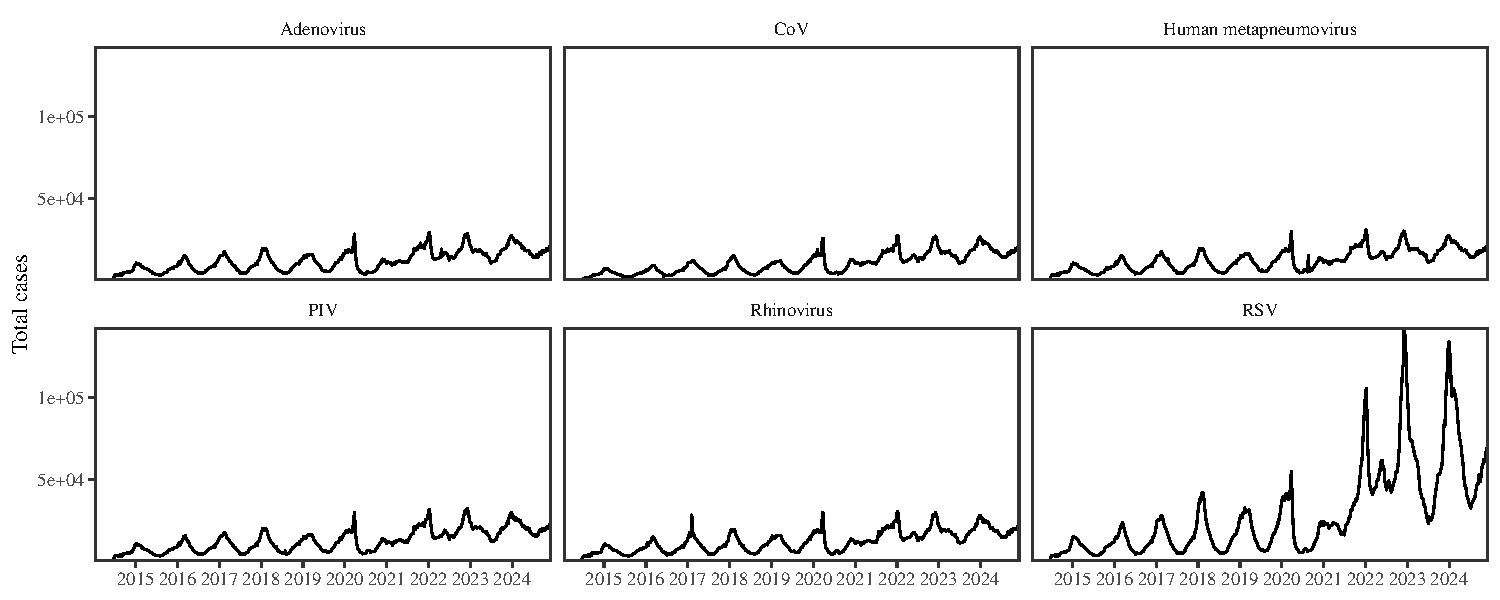
\includegraphics[width=\textwidth]{../figure_test/figure_test_nrevss.pdf}
\caption{
\textbf{Testing patterns for respiratory pathogens in the US reported through the NREVSS.}
}
\end{center}
\end{figure}

\pagebreak

\bibliography{return-time.bib}

\end{document}
